%\documentclass[12pt]{article}
\documentclass[Lau,oneside,italian]{sapthesis}
\usepackage[italian]{babel}
\usepackage[utf8]{inputenc}
\usepackage{graphicx}
\usepackage[sorting=none]{biblatex}
\usepackage{pgfplots}
\usepackage{hyperref}
\usepackage{makeidx}
\usepackage{mathtools}
\usepackage{caption}
\usepackage{subcaption}
\usepackage[outline]{contour} % http://ctan.org/pkg/contour
\makeindex


%\addbibresource{article.bib}
\addbibresource{biblio.bib}


%\title{FloodNet: Deep Learning applicato a immagini aeree}
\title{Approccio basato su Deep Learning per la Segmentazione Semantica di Immagini Aeree}
\author{William De Vena}
\date{2022}

\renewcommand*\contentsname{Indice}


\begin{document}

\IDnumber{1862820}
\course{Informatica} 
\courseorganizer{Facoltà di Ingegneria dell’Informazione, Informatica e Statistica}
\AcademicYear{2021-2022}


\advisor{Prof. Danilo Avola} 
%\customadvisorlabel{Responsabile}


\coadvisor{Prof. Luigi Cinque} \coadvisor{Dott. Alessio Fagioli}
%\customcoadvisorlabel{Corresponsabile} 

\examdate{.} 

\authoremail{william98wdv@gmail.com}
\copyyear{2022} 




\maketitle

%\dedication{GRAZIE}

%\abstract{ABSTRACT}

%\chapter{Introduzione}

\tableofcontents

\chapter{Introduzione}
\section{Contesto di applicazione}
Nel ventennio dal 1995 al 2015, circa il 90\% dei disastri che hanno colpito la popolazione mondiale sono stati causati da fenomeni meteorologici quali inondazioni, tempeste, ondate di caldo ed altri. In questo periodo, l’EM-DAT (Emergency Events Database), uno  dei più importanti database di eventi disastrosi mondiali, ha registrato 6457 disastri causati da eventi meteorologici, che hanno causato 606,000 vittime (una media di 30,000 all’anno) e all’incirca 4.1 miliardi di persone totali colpite (tra il 1995 e il 2015) tra feriti, persone lasciate senza una dimora e persone in bisogno di assistenza.
Tra questi eventi, le alluvioni sono tra le più frequenti e gravi, infatti costituiscono il 43\% del totale degli eventi (Figura \ref{fig:floods}) e hanno causato all’incirca 157,000 morti più 2.3 miliardi di persone colpite (tra il 1995 e il 2015) (Figura \ref{fig:flood_damage}). 
\begin{figure}[h!]
  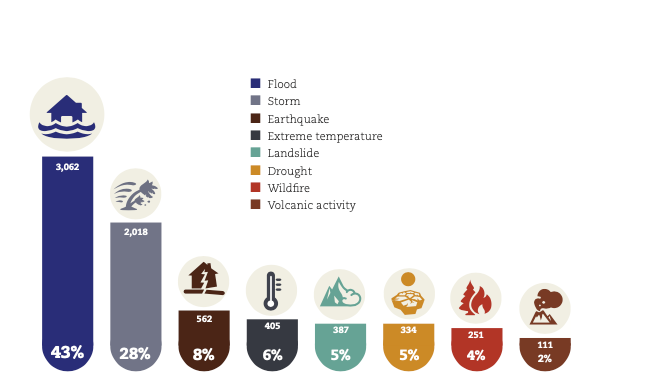
\includegraphics[scale=0.65]{img/stat1.png}
  \caption{Percentuale di eventi di calamità naturali per tipo di disastro  (1995-2015) \cite{2015human}.}
  \label{fig:floods}
\end{figure}
Le alluvioni sono tra le tipologie più gravi anche dal punto di vista dei danni economici, infatti, solo negli Stati Uniti si sono registrati 662 miliardi di dollari di danni causati da alluvioni (1995-2015) e nel continente europeo all’incirca 262 miliardi (1994-2015). Inoltre, le occorrenze di eventi disastrosi causati da fenomeni meteorologici risultano in crescita, in particolare, nel periodo tra il 2005 e il 2014 si è registrata una media di 335 eventi all’anno, ovvero il 14\% in più rispetto al periodo tra il 1995-2004 e quasi il doppio di quelli registrati tra il 1985 e il 1994. Lo stesso trend si può vedere nelle alluvioni, che nello stesso periodo (2005-2014) hanno raggiunto un picco di 171 eventi all’anno, rispetto ai 127 dei decenni precedenti \cite{2015human}.



\begin{figure}[h!]
    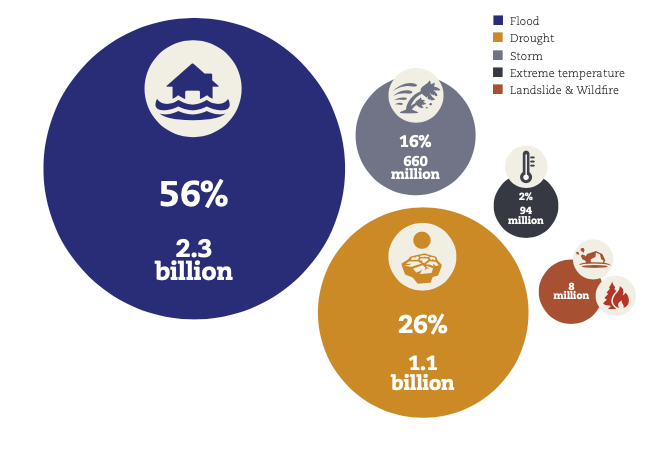
\includegraphics[scale=0.6]{img/stat2.png}
    \caption{Numero di persone colpite da calamità meteorologiche (1995-2015) (NB: i decessi sono esclusi dal totale delle vittime) \cite{2015human}.}
    \label{fig:flood_damage}
\end{figure}


In questo contesto, risulta essenziale la gestione di questi eventi disastrosi. In particolare, sono fondamentali le tre fasi di gestione delle alluvioni: la fase precedente all’evento, ovvero la fase di prevenzione; la fase durante l’evento stesso, in cui è fondamentale avere conoscenza sulle aree colpite e sul propagarsi dell’alluvione, informazioni che spesso non sono facili da reperire; e infine la fase post-alluvione, in cui si valutano i danni. Negli ultimi anni, nel campo della gestione dei disastri naturali, è risultato molto utile l’impiego di UAV (Unmanned Aerial Vehicle), anche chiamati droni. Uno dei primi utilizzi è stato nel 2005 negli Stati Uniti dove, per la prima volta, i droni sono stati utilizzati dal CRASAR (Center for Robot-Assisted Search and Rescue) dell’Università A\&M del Texas per cercare e soccorrere sopravvissuti agli eventi causati dall’Uragano Katrina. Successivamente, nel 2015, il CRASAR ha collaborato con la Measure UAV consulting firm e l’American Red Cross (ARC) per testare le capacità degli UAV in situazioni di emergenza ed eventi disastrosi, il report che ne seguì descrisse i droni come una tecnologia che portò “immediati benefici” sia ai civili che ai soccorritori. Fino ad oggi, i droni sono stati utilizzati in molti eventi di questo tipo, tra i tanti vi sono il terremoto di Wenchuan del 2008, la crisi di Fukushimi Daiichi del 2011 e la gestione del disastro causato dal Tifone Haiyan nelle Filippine nel 2013.
Infatti ad oggi, molte organizzazioni, principalmente umanitarie, hanno lanciato programmi che hanno come obiettivo quello di integrare gli UAV nelle operazioni di gestione di questi eventi, tra queste: l’WFP (ONU World Food Programme), la Banca Mondiale, l’UNHCR (UN High Commissioner for Refugees). In particolare, i droni hanno trovato utilità in tutte e tre le fasi menzionate precedentemente: nella fase di prevenzione vengono spesso utilizzati per monitorare il letto dei fiumi o altri bacini; durante le alluvioni vengono invece utilizzati per mappare le aree colpite, per operazioni di ricerca e soccorso, per il trasporto di carichi in zone altrimenti non raggiungibili, per fornire informazioni in tempo reale dall’alto sullo stato delle strade per guidare le squadre di soccorso, ma anche per fornire informazioni sugli edifici più colpiti per priorizzare le operazioni; infine, nel post-alluvione per la valutazione dei danni \cite{droneappl}.
%\section{Task}
%\label{section_task}
Uno dei principali vantaggi dei droni risiede nella rapidità del loro impiego e nell’alta risoluzione delle immagini che possono catturare. In particolare, con essi si riesce ad ottenere immagini di più alta risoluzione delle aree colpite ed in tempi più brevi rispetto ad altre risorse, come le immagini satellitari \cite{flyhurricane}. Inoltre, con l’elaborazione di queste immagini e grazie alla loro alta risoluzione, si riescono ad estrapolare informazioni molto importanti in questo ambito. Ad esempio, tra i vari utilizzi, si possono distinguere gli edifici e le strade allagate rispetto a quelle non allagate, si possono individuare alcuni oggetti di interesse quali persone o veicoli, oppure si può classificare il livello di danni di un edificio. Infatti, questo lavoro riguarda la segmentazione semantica, una delle tipologie di elaborazioni che spesso viene applicata alle immagini, per fornire informazioni molto utili soprattuto nella fase durante l'alluvione \cite{semsegsurvey}. La segmentazione semantica non è altro che la classificazione di ogni singolo pixel dell’immagine in una delle predeterminate classi (Figura \ref{fig:semseg})  e si distingue dal task della classificazione, in quanto quest’ultima riguarda l’assegnazione di una singola classe all’intera immagine. In particolare, il modello d’interesse di questo lavoro si occupa dell’assegnazione ad ogni pixel dell’immagine di una delle seguenti 9 classi: edificio allagato, edificio non allagato, strada allagata, strada non allagata, acqua, albero, veicolo e prato. Di queste, risultano di forte interesse nell'ambito della gestione di eventi di alluvione soprattutto le prime quattro classi, in quanto distinguere quali edifici siano allagati da quali no, può risultare fondamentale per guidare e priorizzare le operazioni di soccorso, mentre individuare le strade allagate può invece essere utile per distinguere quali strade siano percorribili via terra.

\begin{figure}[h!]
 \centering
 \begin{subfigure}[b]{0.45\textwidth}
     \centering
     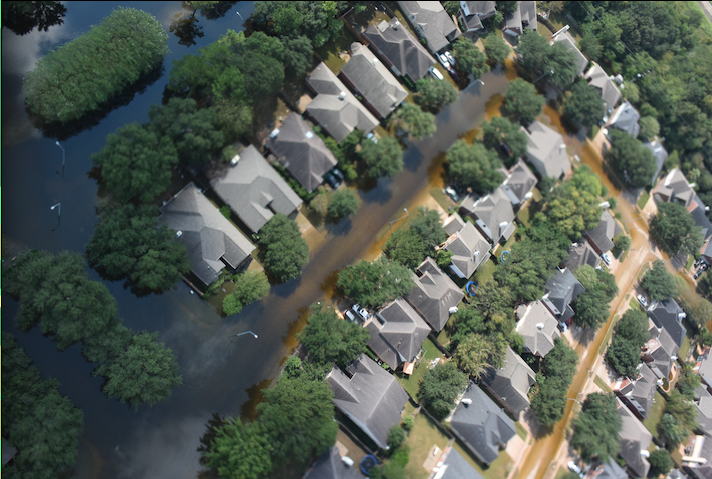
\includegraphics[width=\textwidth]{img/sem_seg copia 2.png}
     \caption{}
     \label{}
 \end{subfigure}
 \hfill
 \begin{subfigure}[b]{0.45\textwidth}
     \centering
     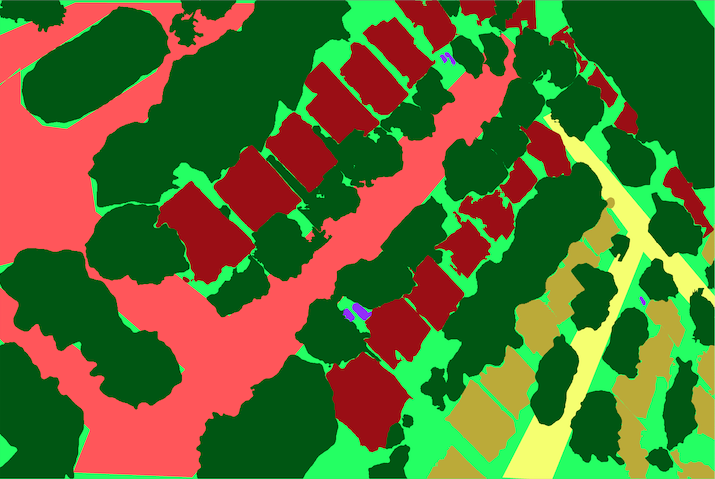
\includegraphics[width=\textwidth]{img/sem_seg copia.png}
     \caption{}
     \label{fig:bottleneck}
 \end{subfigure}
    \caption{Un esempio di segmentazione semantica. La (a) mostra l'immagine in input e la (b) l'output del modello, dove ogni colore corrisponde ad una classe: strada allagata (rosso chiaro), edificio allagato (rosso scuro), strada non allagata (giallo chiaro), edificio non allagato (giallo scuro), albero (verde scuro), prato (verde chiaro), veicolo (viola).}
    \label{fig:semseg}
\end{figure}
















\section{Stato dell'arte}
\label{stato_dell'arte}

Come vedremo più avanti, le reti neurali rispetto ai metodi più tradizionali riescono a cogliere informazioni di più alto livello. In particolare, la loro complessa architettura gli permette di approssimare pattern molto complessi, che i metodi tradizionali non riescono a cogliere. Infatti, come vedremo in questo paragrafo, nello stato dell'arte della segmentazione semantica di immagini aeree, la maggior parte delle metodologie utilizzate sono di Deep Learning.
Una delle architetture più presenti in letteratura e utilizzate in questo campo è la UNet. In diversi lavori \cite{safe_landing, uavid, kattenborn2019convolutional} viene utilizzata la versione classica proposta in \cite{unet}, in altri invece vengono utilizzate delle varianti. Ad esempio, in \cite{rescuenet} viene utilizzata la versione con l'aggiunta del meccanismo di attenzione, chiamata AttentionUnet \cite{attentionUnet}; in \cite{unet-segnet} viene utilizzata in combinazione con la SegNet \cite{segnet} per costruire un'architettura di tipo encoder-decoder (Figura \ref{fig:segnet-unet}); infine viene ripresa in \cite{real-time}, in cui viene utilizzata la rete MobileNet \cite{mobilenet} come backbone, ovvero come la prima parte della UNet (l'encoder) responsabile dell'estrazione delle feature. Ritornando invece su \cite{rescuenet}, il dataset RescueNet viene utilizzato come benchmark per diversi modelli tra cui, oltre all'AttentionUnet, la PSPNet \cite{pspnet}, la DeepLabV3+ \cite{deeplabv3+} e la ENet \cite{enet}. In altri lavori invece, vengono utilizzate architetture ensemble composte da più modelli. In particolare, in \cite{ensemble-cnns} un ensemble di CNN viene testato sul S-PRS Vaihingen Dataset. In questo caso l'ensemble è costituito da più versioni dello stesso modello, ovvero la stessa architettura addestrata più volte sullo stesso dataset  ma con inizializzazioni diverse. 


\begin{figure}[h!]
    \centering
    \hspace*{0in}
    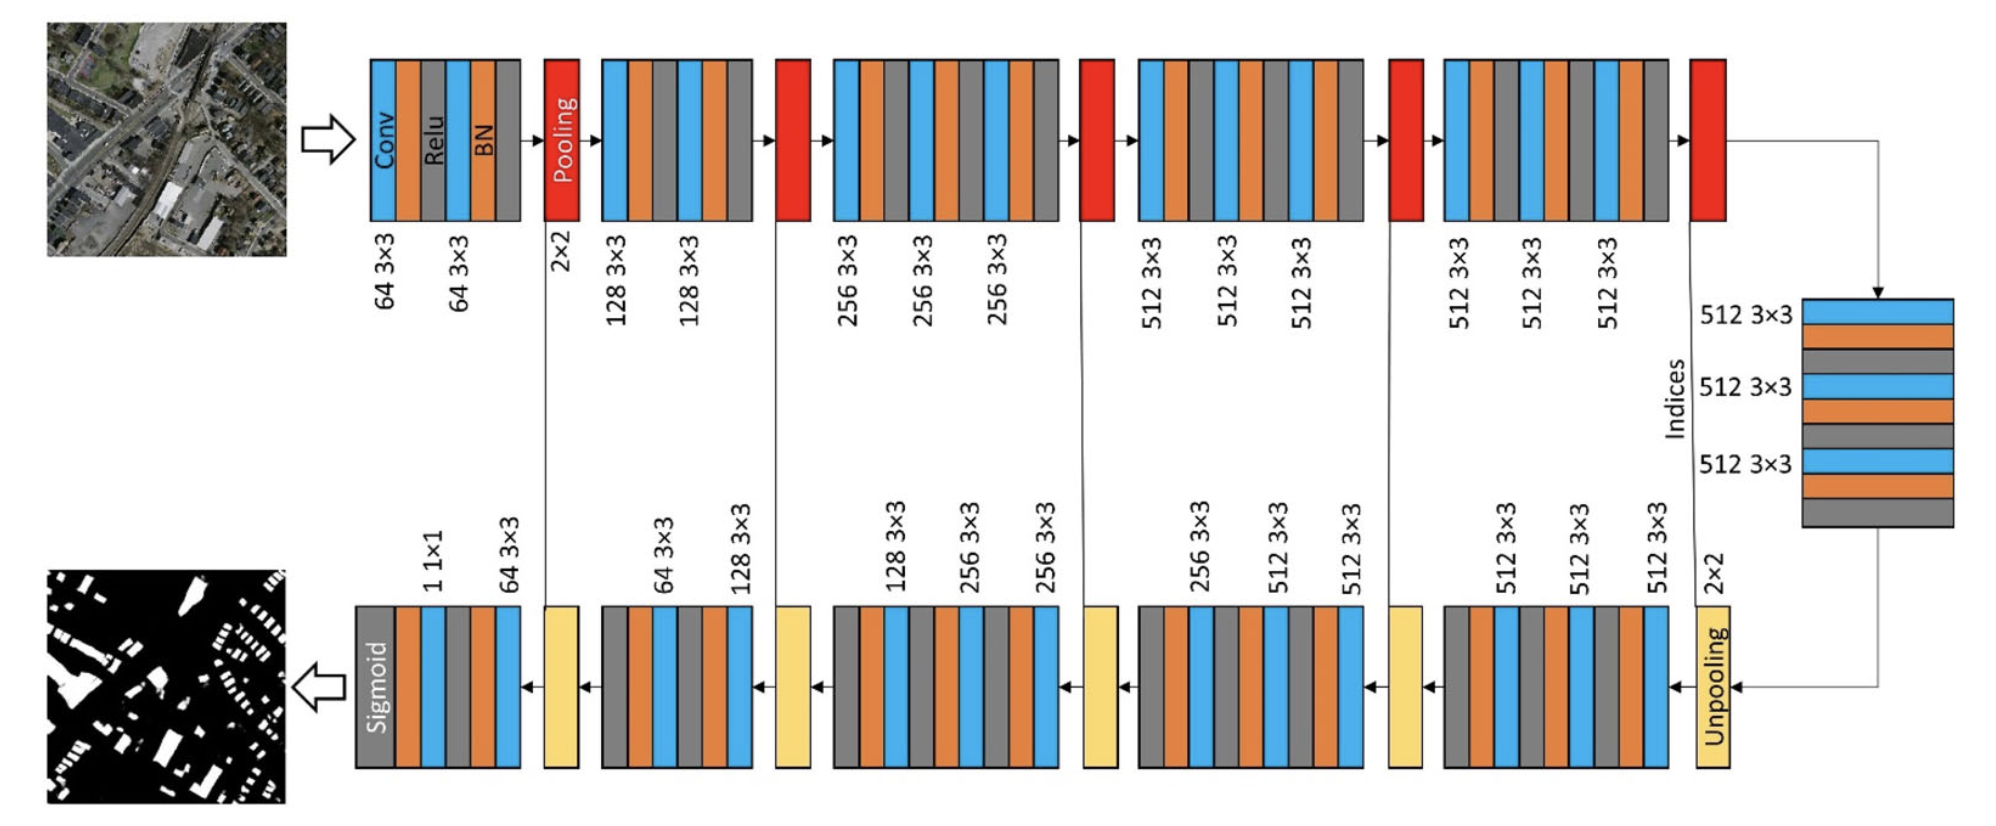
\includegraphics[scale=0.39]{img/segnet+unet.png}
    \caption{Architettura del modello Seg-Unet proposto in \cite{unet-segnet} con una combinazione dei componenti della Segnet (pooling indices) e quelli della Unet (skip connection).}
    \label{fig:segnet-unet}
\end{figure}


L'idea degli autori è che, essendo lo spazio della loss function in cui si muove il modello estremamente non convesso, a molte dimensioni e con molti minimi locali, inizializzare un modello con parametri diversi significa quasi avere la garanzia che convergerà in punti diversi. Di conseguenza, il loro approccio consiste nell'addestrare queste diverse versioni del modello per poi, in fase di inferenza, prendere la media delle loro predizioni. Un simile approccio viene utilizzato anche in \cite{shuffling-cnns}, in cui l'ensemble è composto dallo stesso modello ma preso in diverse fasi dell'addestramento. In particolare, gli autori evidenziano come, con questo approccio, sia possibile addestrare un ensemble senza aggiungere ulteriore tempo rispetto ad addestrare un singolo modello. Così come in \cite{rescuenet}, anche in \cite{hybrid-attention, luo2019high} vengono utilizzati modelli che si basano sul meccanismo di attenzione \cite{attention}. In particolare, gli autori  di \cite{hybrid-attention} evidenziano come un meccanismo  di attenzione ibrido, ovvero l'unione di diverse tipologie di attenzioni (sui canali, sullo spazio e sulle classi) riesca a catturare dipendenze a lungo raggio, aiutando così il modello a produrre delle feature map di qualità. Dall'altra parte, in \cite{luo2019high} gli autori, oltre a proporre un modello basato sulla struttura di una FCN con l'aggiunta del meccanismo di attenzione sui canali (\textit{channel attention mechanism}), propongono una approccio basato sull'utilizzo di due tipologie di dati corrisposte da due tipologie di backbone. In particolare, la prima parte del modello è composta da due ResNet101, una che prende in input l'immagine e una che invece prende in input dati ausiliari come l'NDVI (Normalized Difference Vegetation Index) ed altri. Nella seconda parte invece, le due feature map vengono concatenate e passate al modulo di \textit{channel attention}, per poi passare infine nella parte di upsample per produrre le maschere finali (Figura \ref{fig:channel_attention}).

\begin{figure}[h!]
    \centering
    \hspace*{0in}
    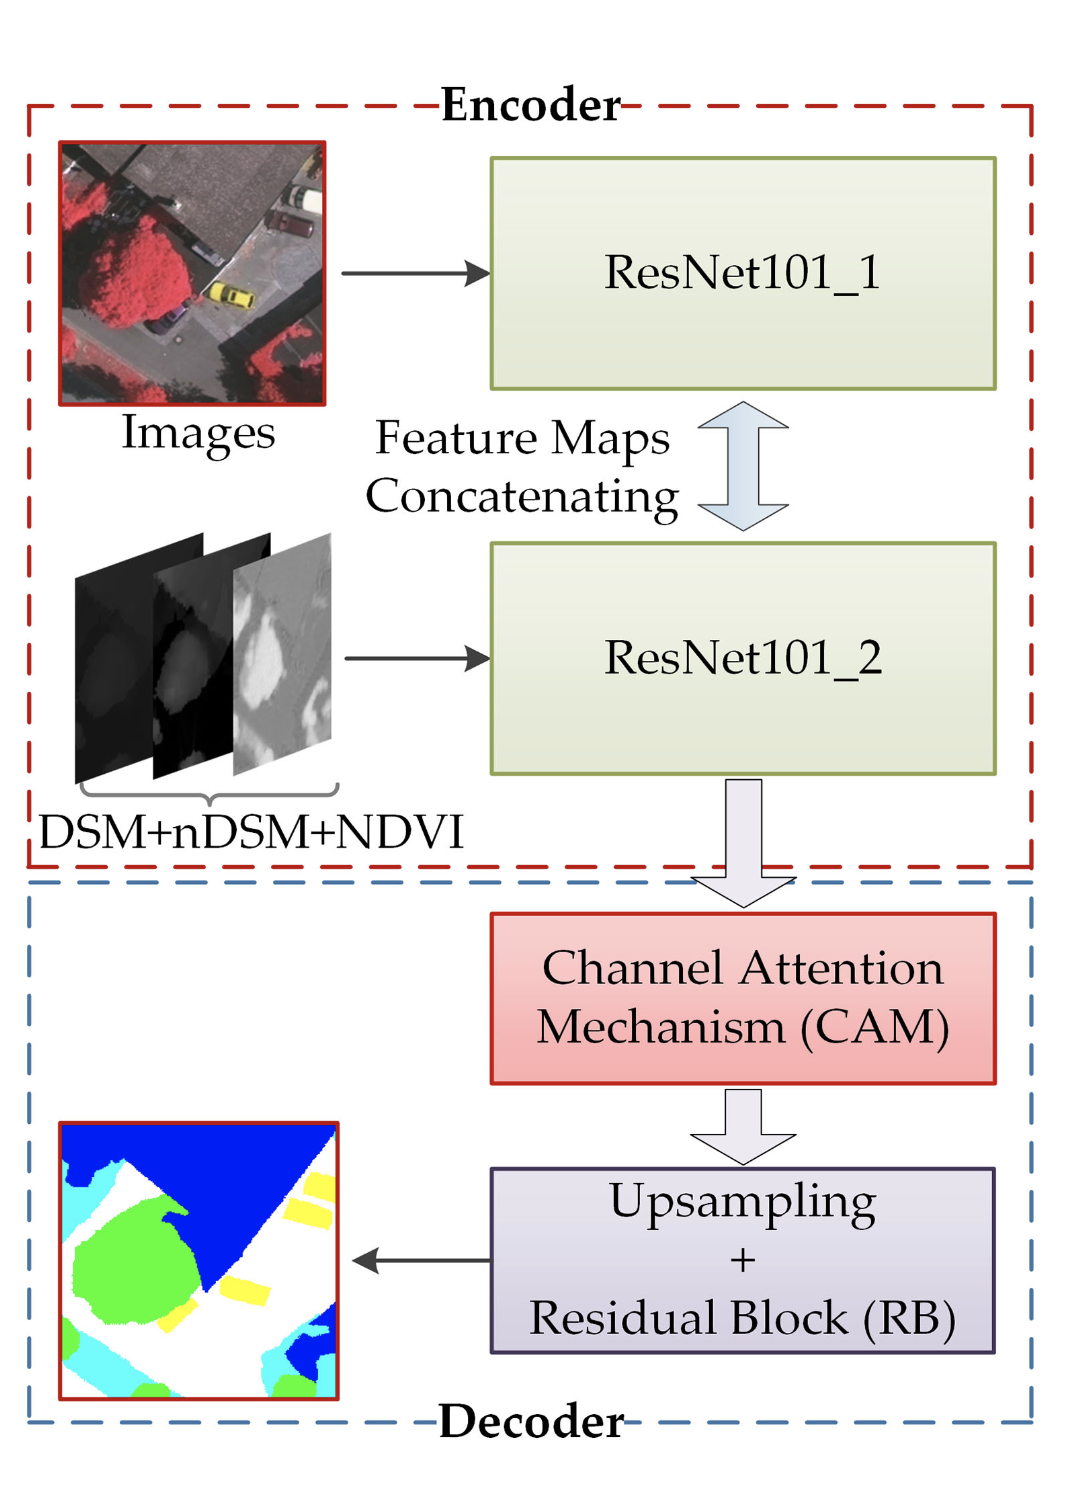
\includegraphics[scale=0.3]{img/chanel_attention_archi.png}
    \caption{Archittetura del modello basato sull'uso del \textit{channel attention mechanism} proposto in \cite{luo2019high}.}
    \label{fig:channel_attention}
\end{figure}





In \cite{distance_map} le maschere all'interno del dataset, prima di essere utilizzate per addestrare il loro modello, subiscono una prima fase di processing in cui vengono trasformate in delle \textit{distance maps}. In particolare, per ogni maschera e per ogni classe viene prodotta una maschera binaria, i cui valori dei pixel rappresentano la distanza di quel pixel di quella determinata classe dal bordo dell'oggetto di cui fa parte (Figura \ref{fig:distance_maps}).

\begin{figure}[h!]
    \centering
    \hspace*{-0.2in}
    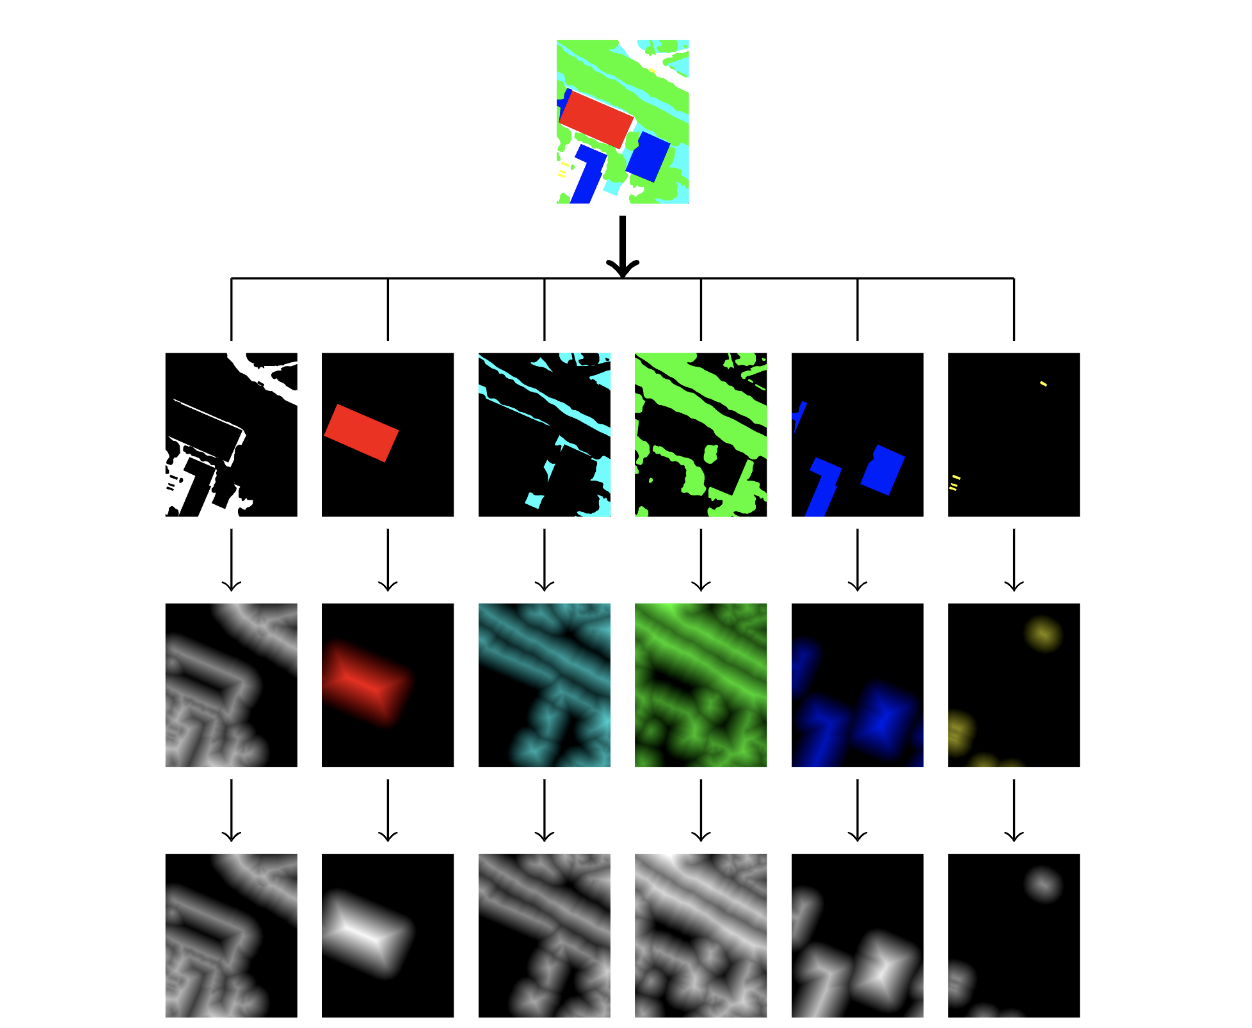
\includegraphics[scale=0.56]{img/distance_mps.png}
    \caption{Illustrazione della produzione di una \textit{distance map} a partire da una maschera \cite{distance_map}.}
    \label{fig:distance_maps}
\end{figure}

La motivazione per cui utilizzare le distance maps è che, grazie al fatto che codificano informazioni spaziali in più rispetto alle semplici maschere, gli output del modello ottenuto dal loro utilizzo nell'addestramento risultano con meno rumore, con più coerenza spaziale e i bordi degli oggetti appaiono più definiti (Figura \ref{fig:distance_map_result}).

\begin{figure}[h!]
     \centering
     \begin{subfigure}[b]{0.45\textwidth}
         \centering
         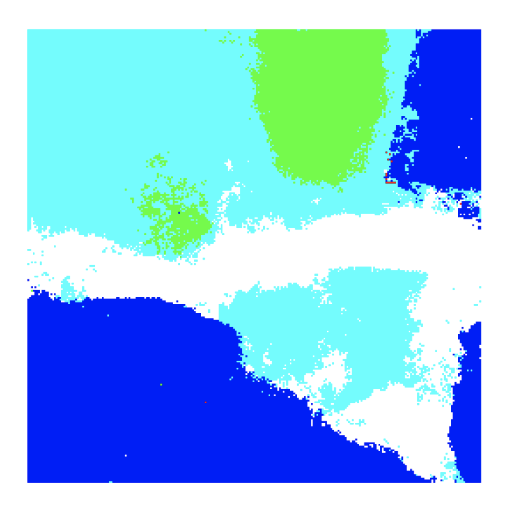
\includegraphics[width=\textwidth]{img/distance3.png}
         \caption{}
         \label{}
     \end{subfigure}
     \hfill
     \begin{subfigure}[b]{0.45\textwidth}
         \centering
         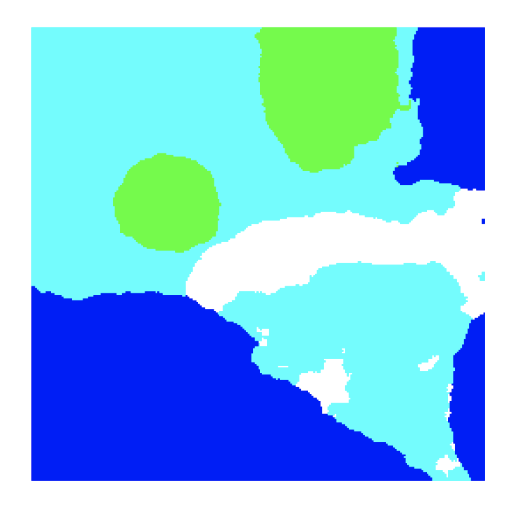
\includegraphics[width=\textwidth]{img/distance2.png}
         \caption{}
         \label{}
     \end{subfigure}
        \caption{La figura mostra il risultato del modello senza l'utilizzo delle \textit{distance maps} (a) e il risultato del loro utilizzo (b) \cite{distance_map}.}
        \label{fig:distance_map_result}
\end{figure}

Una variante della segmentazione semantica è quella affrontata in \cite{towards}, ovvero la segmentazione semantica open-set, che consiste nel task della segmentazione semantica, con l'aggiunta del fatto che il numero totale di classi è sconosciuto. Di conseguenza, la segmentazione semantica open-set può essere descritta come il task in cui ogni pixel può essere etichettato come appartenente a una delle classi apprese durante l'addestramento, oppure come una classe sconosciuta.
Le difficoltà di questa tipologia di task evidenziate dagli autori sono principalmente: la diversità di pattern nella classe sconosciuta e la similarità tra i pattern delle classi conosciute e quelli delle classi sconosciute. L'approccio proposto dagli autori consiste nel segmentare l'immagine con una CNN, che classifica pixel per pixel, e determinare una soglia per la quale se l'output della softmax della CNN non la supera, quel pixel viene classificato come classe sconosciuta. In aggiunta, propongono anche un ulteriore step per migliorare la qualità delle maschere prodotte e diminuire il numero di pixel della classe sconosciuta. In particolare, il metodo proposto, chiamato \textit{Morphological Filtering}, consiste nel riassegnare ogni pixel alla classe più presente nel suo vicinato e, nella pratica, l'effetto può essere visto come l'erosione della regioni classificate come classe sconosciuta (Figura \ref{fig:erosion}).

\begin{figure}[h!]
    \centering
    \hspace*{-0.17in}
    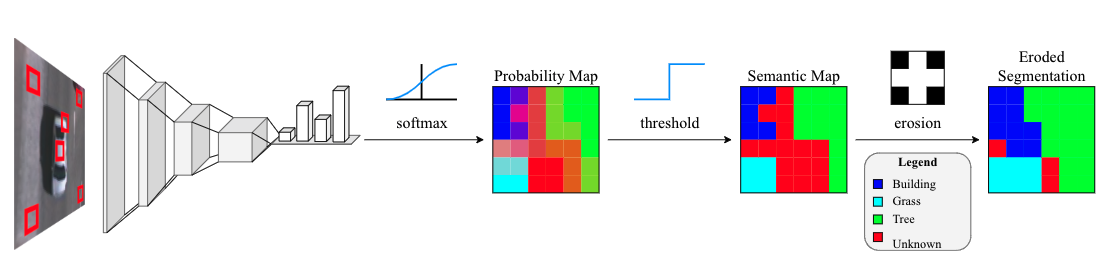
\includegraphics[scale=0.35]{img/erosion.png}
    \caption{Illustrazione del metodo proposto in \cite{towards}.}
    \label{fig:erosion}
\end{figure}




Altri lavori, come ad esempio \cite{three_dim}, utilizzano la segmentazione come step intermedio per altri task. In particolare, in quest'ultimo lavoro citato, le maschere prodotte vengono utilizzate per la stima della profondità delle acque di alluvioni e il modello utilizzato è una versione della FCN \cite{FCNs} con stride 8 (FCN-8s) e VGG-16 come backbone. In \cite{deep-based} vengono testate diverse versioni della UNet \cite{unet} e della LinkNet \cite{linknet}, combinando tra loro diversi modelli per la backbone e per la parte di decoder. Inoltre, gli autori hanno mostrato come in media su quasi tutti gli aspetti, i modelli che avevano la backbone pre addestrata su ImageNet abbiano performato meglio. In alcuni lavori invece, come \cite{sem_seg_ML}, oltre ad architetture di Deep Learning, vengono anche testati algoritmi di Machine Learning più tradizionali. Il loro lavoro riguarda il task della segmentazione delle diverse tipologie di vegetazione e, in particolare, il loro approccio è stato quello di testare diversi classificatori di ML, tra cui Random Forest, alberi decisionali e K-nearest neighbor. Per quanto riguarda, invece, l'architettura di Deep Learning da loro utilizzata, si tratta della SegNet \cite{segnet}. Infine, in \cite{floodnet} viene affrontato lo stesso specifico task di questo lavoro, ovvero il dataset FloodNet. In particolare, l'approccio degli autori consiste nel testare varie architetture, tra cui ENet \cite{enet}, PSPNet \cite{pspnet} e DeepLabV3+ \cite{deeplabv3+}. Nello specifico, gli autori evidenziano come le architetture che performano meglio siano quelle context-based e tra queste, la migliore è risultata la PSPNet.





















\section{Contributo ed Outline}
In questo lavoro viene esplorato il task della segmentazione semantica di immagini aeree del dataset FloodNet, attraverso approcci di Deep Learning. Nello specifico, viene proposto un nuovo approccio basato sulla risoluzione delle principali difficoltà individuate nel dataset. 
In particolare, il principale contributo di questo lavoro si può riassumere nei seguenti punti:


\begin{itemize}
    \item una fase di \textit{data cleaning}, per ovviare alla corposa presenza di errori nelle maschere del dataset.
    
    \item una fase di data augmentation offline, utile a far fronte ad un forte sbilanciamento del dataset verso alcune classi e alla presenza di altre in misura notevolmente minore.
    
    \item utilizzo di un'architettura context-based, mai utilizzata su questo dataset, volta ad ovviare alle difficoltà intrinseche di particolari classi, la cui semantica è fortemente basata sul loro contesto.
\end{itemize}

Per quanto riguarda la struttura dell'elaborato, esso è stutturato come segue. Nel Capitolo \ref{chapter_seg}, verrà esplorato il problema generale della segmentazione trattando le varie metodologie esistenti, sia tradizionali sia di Deep Learning. In seguito, nel Capitolo \ref{deep_learning}, si tratteranno i principali concetti di Deep Learning, approfondendo anche alcune delle architetture più note. Nel Capitolo \ref{chap_archi} invece, si entrerà nel dettaglio del task specifico di questo lavoro e si mostreranno, oltre all'architettura, anche le principali metodologie utilizzate.
Successivamente, nel Capitolo \ref{chap_exp} si illustreranno i vari esperimenti fatti durante tutto il lavoro e i loro risultati. Infine, nel Capitolo \ref{chap_conclusion} si trarranno le conclusioni del lavoro.
\chapter{Segmentazione di immagini}
\label{chapter_seg}
 La segmentazione è uno dei task più popolari nel campo del Deep Learning applicato alle immagini e, in generale, nel campo della Computer Vision. In particolare, consiste nel produrre una maschera delle stesse dimensioni dell'immagine in input, dove il valore di ogni pixel rappresenta la classe a cui è stato assegnato, o detto in altre parole, partizionare un'immagine in regioni con un valore semantico ben preciso (Figura \ref{fig:example_sem_seg}).

\begin{figure}[b!]
    \centering
    \hspace*{-0.1in}
    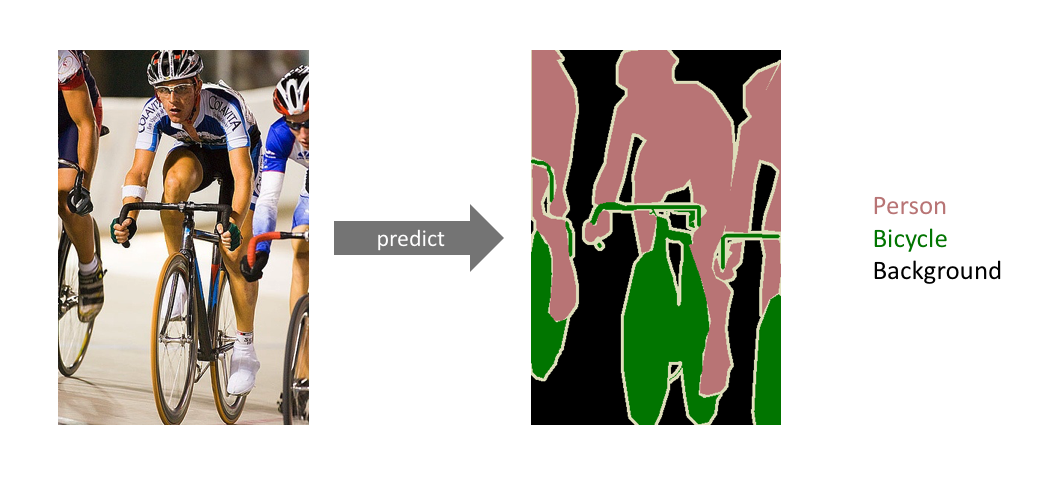
\includegraphics[scale=0.37]{img/example_sem_seg.png}
    \caption{Un esempio del risultato della segmentazione di un'immagine.}
    \label{fig:example_sem_seg}
\end{figure}

Grazie alle informazioni spaziali che si possono ottenere con la segmentazione, molti campi ne beneficiano, tra cui il campo dei veicoli autonomi, la detection di pedoni, diagnosi medica assistita da computer e molti altri \cite{semsegsurvey}. 

%Grazie al fatto che la segmentazione permette di ottenere sull'immagine in input, oltre che informazioni semantiche, anche informazioni spaziali, molti campi ne beneficiano, tra cui, il campo dei veicoli autonomi, la detection di pedoni, diagnosi medica assistita da computer e molti altri \cite{semsegsurvey}. 

%\subsubsection{Tipi di immagini}
In letteratura la segmentazione è stata applicata a una grande varietà di dati. Alcune tra le tipologie più utilizzate sono: 
\begin{itemize}
    \item \textbf{scala di grigi}: un tipo di immagine che presenta un solo canale e il valore dei pixel rappresentano, sostanzialmente, la quantità di luce del pixel.
    
    \item \textbf{RGB (red, green and blue)}: probabilmente la tipologia più nota, presenta tre canali che rappresentano rispettivamente la quantità di rosso, di verde e di blu del pixel.
    
    \item \textbf{RGB-D}: un tipo di immagine che, oltre ad avere i tre canali del RGB, ha anche un quarto canale che rappresenta la profondità di quel pixel, ovvero la distanza dalla camera, informazione spesso molto utile nel campo della segmentazione semantica \cite{qi20173d}.
    
    \item \textbf{3D}: un tipo di dato spesso presente nella letteratura medica, come ad esempio nel campo della TC (tomografia computerizzata), dove le immagini vengono catturate con strumenti a raggi X \cite{hu2001automatic}.
\end{itemize}
%\subsubsection{Dataset di benchmark}
Come detto in precedenza, la segmentazione è uno dei task più popolari e negli anni nel campo della ricerca, sono stati fatti molti passi avanti, sviluppando modelli e algoritmi sempre più performanti. In particolare, le performance di questi modelli sono state misurate testandoli su dei dataset, che sono stati usati come benchmark per paragonare i vari metodi. Tra i dataset di benchmark più noti ed utilizzati ci sono:
\begin{itemize}
    \item \textbf{PASCAL-VOC} (PASCAL Visual Object Classes) \cite{pascal-voc}
    \item \textbf{Cityscapes dataset} \cite{cityscapes}
    \item \textbf{ADE20K} \cite{zhou2019semantic}
\end{itemize}
Nel campo della computer vision, la segmentazione viene affrontata con diversi metodi. In particolare, esistono metodi tradizionali, che non fanno uso di tecniche di Machine Learning; metodi di Machine Learning; e infine metodi di Deep Learning, che sfruttano invece architetture che, come vedremo più avanti, riescono ad apprendere pattern molto complessi che i metodi tradizionali e di Machine Learning spesso non riescono a cogliere.
Per quanto riguarda i metodi tradizionali, le tecniche sono svariate: alcune sono basate sull'estrazione di feature e altre sul preprocessing dell'immagine in input; invece, per quanto riguarda i metodi di Machine Learning, essi sono basati sul trasformare i pixel dell'immagine in una rappresentazione che poi può essere utilizzata dagli svariati algoritmi di Machine Learning per classificarli, come il K-Means o l'SVM (Support Vector Machines). Invece, le architetture di Deep Learning sono diverse e tra le più utilizzate ci sono la UNet\cite{unet}, la DeepLabV3\cite{deeplabv3}, la PSPNet\cite{pspnet}, la FCN\cite{FCNs} e altre. Vedremo più avanti i concetti di Deep Learning sui quali si basano queste architetture.
Al di là delle metodologie utilizzate, un aspetto molto importante dello sviluppare un algoritmo, un'architettura, oppure utilizzarne una già esistente, consiste nella scelta della metrica di valutazione. Di metriche ne esistono diverse:

\begin{itemize}
    \item \textbf{Accuracy}: questa è probabilmente la più semplice e più intuitiva, ovvero misura il numero di pixel correttamente classificati, chiaramente in proporzione al numero totale di pixel. Questa metrica è generalmente una delle più utilizzate nel campo del Machine Learning.
    Viene definita come:
    
    \begin{equation}
        Accuracy = \frac{\sum_{i=1}^k{n_{ii}}}{\sum_{i=1}^k{t_{i}}}.
    \end{equation}
    
    Dove $k$ è il numero di classi, $n_{ij}$ è il numero di pixel di classe $i$ e classificati come di classe $j$ e $t_{i}$ il numero totale di pixel della classe $i$ ovvero:
    
    \begin{equation}
        t_{i} = \sum_{j=1}^k{n_{ij}}.
    \end{equation}
    Inoltre, a parte l'accuracy generale, che in pratica misura l'accuratezza del modello, ma non facendo caso alle singole classi, possiamo anche utilizzare l'accuracy di una classe. In particolare, l'accuracy di una singola classe $i$ è definita come il rapporto tra il numero di pixel di quella classe correttamente classificati dal modello e il numero totale di pixel di quella classe:
    
    \begin{equation}
        Accuracy_{i} = \frac{n_{ii}}{t_{i}}.
    \end{equation}
    
    Il principale svantaggio nell'utilizzo dell'accuracy è che in molti task alcune classi prevalgono rispetto alle altre, di conseguenza utilizzare l'accuracy può portare ad avere un valore alto, ma che in realtà è causato dalla predominanza di quella classe. Ad esempio, se in un'immagine l'80\% dei pixel è di una classe, un modello che classifica tutti i pixel dell'immagine come appartenente a quella classe, otterrebbe una accuracy dell'80\%.
    
    
    \item \textbf{Accuracy media}: questa ed altre metriche fanno fronte al problema sopra menzionato dell'accuracy. Questa metrica, in particolare, rappresenta la media delle accuracy delle singole classi e risolve il problema normalizzando l'accuracy rispetto al numero totale dei pixel:
    
    \begin{equation}
        MeanAccuracy = \frac{1}{k} \sum_{i=1}^k{Accuracy_{i}} = \frac{1}{k} \sum_{i=1}^k{\frac{n_{ii}}{t_{i}}}.
    \end{equation}
    
    
    \item \textbf{Mean intersection over union (mIoU)}: anche chiamato \textit{Jaccard index}, è la media dell'\textit{intersection over union (IoU)} dell $k$ classi, dove l'IoU di una classe è essenzialmente il rapporto tra l'intersezione e l'unione di due insiemi: l'insieme dei pixel di quella classe nella maschera e l'insieme dei pixel di quella classe nella predizione, ovvero:
    
    \begin{equation}
        IoU = \frac{target \cap prediction}{target \cup prediction}.
    \end{equation}
    
    definibile anche come
    
    \begin{equation}
        IoU = \frac{n_{ii}}{t_{i}-n_{ii}+\sum_{j=1}^k{n_{ij}}}.
    \end{equation}
    
     e di conseguenza la mIoU è definita come:
     
     \begin{equation}
         mIoU = \frac{1}{k} \sum_{i=1}^k{IoU_{i}} =
         \frac{1}{k} \sum_{i=1}^k{\frac{n_{ii}}{t_{i}-n_{ii}+\sum_{j=1}^k{n_{ij}}}}.
     \end{equation}
     
     
    \item \textbf{Frequency weighted intersection over union (FWIoU)}: una variante della mIoU, che invece di calcolare semplicemente la media delle IoU, calcola una media pesata rispetto al numero di pixel delle classi (frequenza), ovvero:
    
    \begin{equation}
        FWIoU = (\sum_{i=1}^k{t_{i}})^{-1} \sum_{i=1}^k{t_{i}IoU_{i}} = (\sum_{i=1}^k{t_{i}})^{-1} \sum_{i=1}^k{t_{i}\frac{n_{ii}}{t_{i}-n_{ii}+\sum_{j=1}^k{n_{ij}}}}.
    \end{equation}
    
    
    \item\textbf{Matrice di confusione}: non è una vera e propria metrica, ma è un metodo molto utilizzato anche e soprattutto nel campo della classificazione. La matrice di confusione è molto utile in particolare quando si vuole approfondire la natura degli errori del proprio metodo. Nello specifico, ci mostra per ogni classe $i$ il numero di pixel correttamente predetti $n_{ii}$ ma, ancora più importante, per ogni classe ci mostra la suddivione degli errori nelle altre classi, ovvero $n_{ij}$ per $j \in [1,2,..., i-1, i+1, ..., k]$. Di conseguenza, possiamo rappresentare formalmente la matrice di confusione come:
    
    \begin{equation}
        ConfusionMatrix = [n_{ij}].
    \end{equation}
    
    dove  $i,j \in [1, 2, ..., k]$.
    
\end{itemize}

Inoltre, nel campo della Computer Vision, così come nel mondo algoritmico, i metodi vengono valutati secondo due ulteriori criteri: la complessità temporale, molto importante soprattutto in alcuni campi di applicazione dove il tempo necessario per processare un'immagine e produrre la sua segmentazione non deve essere maggiore di una certa soglia, come il campo dei veicoli autonomi; e la complessità spaziale, ovvero la quantità di memoria di cui ha bisogno l'algoritmo, metrica molto importante soprattutto in campi dove il processamento avviene su dispositivi che non abbondano di memoria, come smartphones e fotocamere.












\section{La segmentazione di immagini negli umani}
Partendo da come gli umani percepiscono un'immagine e riescono naturalmente e in modo intuitivo a segmentarla, il funzionamento di tali intuizioni si basa su quella che è chiamata "psicologia della Gestalt" \cite{gestalt} (dal tedesco \textit{Gestaltpsychologie}, 'psicologia della forma' o 'rappresentazione'). La piscologia della Gestalt spiega come un umano riesca a percepire un'immagine e organizzarla in un sistema complesso. In particolare, spiega come, guardando il mondo intorno a sé, riesca a percepire scene complesse composte da molti gruppi di oggetti su uno sfondo, che a loro volta possono essere costituiti da altre parti e via dicendo.
Il modo in cui gli umani riescano a raggiungere un risultato percettivo così notevole, visto il fatto che l'input visivo è, in un certo senso, solo una distribuzione spaziale di punti individuali variamente colorati, è basato su dei principi che definiscono le intuizioni dietro il raggruppamento di parti dell'immagine. Non esiste una lista precisa dei principi della Gestalt, ma ne esistono alcuni che sono più discussi e più comunemente utilizzati \cite{todorovic2008gestalt}:

\begin{itemize}
    \item \textbf{principio di buona forma}: la struttura di oggetti che tendiamo a percepire è sempre la più semplice.

    \item \textbf{principio di prossimità}: formalizza l'intuizione dietro il fatto che tendiamo a raggruppare elementi vicini tra loro.
    
    \item \textbf{principio di destino comune}: tendenza a raggruppare elementi che hanno un movimento coerente tra loro.
    
    \item \textbf{principio di somiglianza}: tendenza a raggruppare gli elementi simili tra loro (in colore, forma, grandezza, ...)
    
    \item \textbf{principio di buona continuità}: tendenza a raggruppare elementi per formare oggetti e forme continue e coerenti nello spazio.
    
    \item \textbf{principio dell'esperienza passata}: l'osservatore tende a raggruppare gli elementi visivi in modo coerente al modo in cui li ha visti nel suo passato.
\end{itemize}

In generale, questi principi formalizzano delle intuizioni comuni alla piscologia di tutti gli umani. Il problema è che queste intuizioni sono spesso molto difficili da trasformare in un linguaggio matematico o in un algoritmo, e da qui nasce la difficoltà della segmentazione e di altri task nel campo della Computer Vision, che come quest'ultima risultano spesso intuitivi, ma molto difficili da trasformare in un algoritmo.
Inoltre, anche per gli umani, a volte, il task della segmentazione risulta complesso e i risultati, quando cambia il soggetto, sono spesso diversi tra loro.  Questo ci fornisce un'intuizione di come, a differenza di altri task come la classificazione, il problema della segmentazione sia particolarmente difficile anche solo da definire \cite{martin2001database}.







\section{Approcci classici}
Come detto in precedenza, il task della segmentazione d'immagini può essere affrontato con diversi approcci classici. Alcuni di questi trasformano il task in un problema di ottimizzazione, cercando poi di risolverlo con algorimi iterativi,  altri invece lo trasformano in un problema di \textit{clustering}, trasportando l'immagine in uno spazio a più dimensioni per poi utilizzare algoritmi di Machine Learning. 







\subsection{Metodi a soglia}
\label{metodi_soglia}
Uno dei metodi più semplici e intuitivi è il metodo a soglia (\textit{thresholding}). In pratica, esso consiste nel definire una soglia numerica di una feature dell'immagine, per poi classificare i pixel in base a questa soglia. Nella sua forma più semplice, definendo un'unica soglia l'immagine viene segmentata in due classi; nella sua variante multiclasse, invece, si definiscono più soglie, creando così degli intervalli che rappresentano le diverse classi. La feature utilizzata più spesso è quella dell'intensità dei pixel (in immagini in scala di grigi), ma se ne possono utilizzare tante altre, questo dipende molto dal campo di applicazione e dalla natura dell'immagine. Ad esempio, una feature spesso molto utile per segmentare un'immagine è la profondità. Il problema principale consiste nel fatto che questo tipo di feature, a parte il caso in cui sia fornito direttamente dall'immagine (RGB-D), è spesso molto difficile da estrarre.
Chiaramente, questo metodo restituisce spesso risultati approssimativi e inoltre la ricerca del valore ottimale della soglia non è affatto semplice e richiede spesso un'approfondita conoscenza del dominio.





\subsection{Metodi dividi e fondi}
\label{metodi_dividi_fondi}
Come abbiamo visto nel paragrafo precedente, una delle tecniche più semplici è definire una soglia con cui classificare i pixel. Sfortunatamente, nella maggior parte dei casi trovare questa soglia è molto difficile e molto spesso non è nemmeno unica, ovvero le immagini a volte presentano forti differenze da una regione all'altra, di conseguenza una buona soglia per una parte può risultare non buona per un'altra. 
Data questa difficoltà, una tecnica per risolverla consiste nel suddividere l'immagine in parti diverse oppure, al contrario, cercare di unire parti di immagine simili tra loro.
Uno dei primi algoritmi che rientra in questa categoria è l'algoritmo degli spartiacque (in inglese \textit{watershed}) \cite{watershed}, che considera le immagini in scala di grigi come una mappa topografica, trasformando l'intensità dei pixel nell'altezza. In particolare, utilizzando la metafora di un'alluvione, l'algoritmo suddivide l'immagine in diversi bacini idrografici, ovvero le regioni segmentate delle immagini sono composte da tutti quei punti da cui l'acqua finirebbe nello stesso punto (il minimo) (Figura \ref{fig:watershed}). Sfortunatamente, anche questo algoritmo spesso restituisce risultati approssimativi, in particolare, uno dei maggiori problemi è che, associando una regione ad ogni minimo locale, spesso over-segmenta l'immagine. Infatti, questo algoritmo è soprattutto usato in sistemi interattivi dove la segmentazione è assistita da un utente che definisce il centro degli oggetti d'interesse.
\\ \\
\begin{figure}[h!]
    \centering
    \hspace*{-0.1in}
    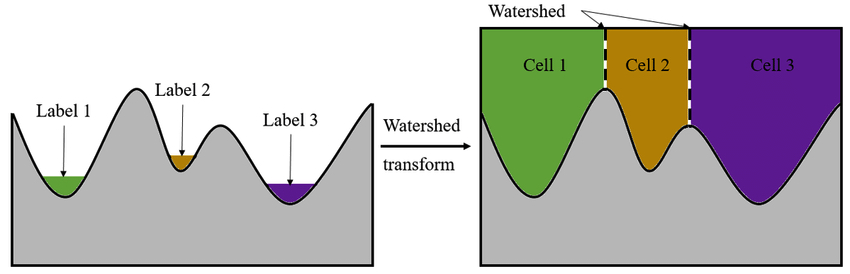
\includegraphics[scale=0.4]{img/watershed2.jpg}
    \caption{Illustrazione di come l'algoritmo degli spartiacque trova le soglie (watershed nell'immagine) con cui segmentare le immagini.}
    \label{fig:watershed}
\end{figure}

Infine, ci sono altri metodi che, invece che cercare di suddividere l'immagine in regioni, cercano al contrario di unire tra loro regioni che abbiano una certa similarità con un approccio \textit{bottom-up}. Una categoria di questi sono i metodi basati su grafi.




\subsection{Metodi basati su grafi}
\label{metodi_grafi}
Questa categoria di metodi si basa sulla rappresentazione dell'immagine come un grafo $G=(V,E)$ dove i vertici $V$ sono i pixel e gli archi $E$ sono tra i pixel adiacenti. Uno degli algoritmi che fa parte di questa categoria è quello proposto in \cite{graph_segm}, in cui i pesi rappresentano una misura di dissimilarità tra i pixel che connettono. Questa misura di dissimilarità $w(e)$ può prendere diverse forme e quella più semplice è probabilmente la differenza di intensità tra i due pixel. 
Una qualsiasi regione $R$ ha una misura di differenza interna chiamata $Int(R)$, che è definita come il massimo peso di un arco all'interno dell'albero ricoprente minimo di $R$, ovvero $MST(R)$: 

\begin{equation}
    Int(R) = \max_{e\in MST(R)} w(e).
\end{equation}

Inoltre, per due regioni adiacenti, ovvero che hanno minimo un arco che le connette, si definisce la differenza tra loro come il peso minimo di un arco che le connette:

\begin{equation}
    Dif(R_{1}, R_{2}) = \min_{e=(v_{1}, v_{2}) | v_{1} \in R_{1}, v_{2} \in R_{2}} w(e).
\end{equation}

L'algoritmo unisce iterativamente tra loro due qualsiasi regioni $R_{1}$ e $R_{2}$ se la loro differenza $Dif(R_{1}, R_{2})$ è minore della minima differenza interna delle due regioni $MInt(R_{1}, R_{2})$, dove

\begin{equation}
    MInt(R_{1}, R_{2}) = min(Int(R_{1}) + \tau(R_{1}),  Int(R_{2}) + \tau(R_{1})).
\end{equation}

Dove $\tau(R_{1})$ rappresenta quanto la differenza tra le due regioni debba essere più grande delle differenze interne per non essere fuse, ma segmentate in due regioni diverse, ed è definito come:

\begin{equation}
    \tau(R) = \frac{k}{|R|}.
\end{equation}

Dove $k$ è un paramtero costante e $|R|$ è la dimensione della regione. In realtà, questo componente $\tau$ può assumere diverse forme a seconda dello specifico task e in base a come si voglia definire la bontà di una regione.
Infine, la regola con cui l'algoritmo decide iterativamente di unire o meno due regioni è la seguente: unire $R_{1}$ e $R_{2}$ se $Dif(R_{1}, R_{2})<MInt(R_{1}, R_{2})$.
\\ \\
\begin{figure}[h!]
    \centering
    \hspace*{-0in}
    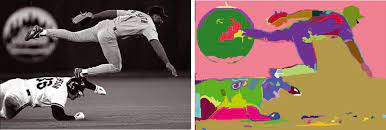
\includegraphics[scale=1]{img/graph_segm.jpeg}
    \caption{Esempio del risultato dell'algoritmo basato su grafi proposto in \cite{graph_segm} applicato su un'immagine in scala di grigi.}
    \label{fig:graph_baseball}
\end{figure}




\subsubsection{Tagli normalizzati}
Un altro algoritmo molto popolare che appartiene a questa categoria è quello proprosto in \cite{shi2000normalized}. In questo algoritmo, il peso di un arco $w_{i,j}$ tra i due pixel $i$ e $j$ rappresenta la loro affinità. L'idea dietro l'algoritmo è partizionare il grafo in regioni che abbiano affinità deboli, ovvero regioni connesse da archi con pesi bassi. Per definire il costo di un taglio tra due regioni $A$ e $B$, viene definita la seguente misura:

\begin{equation}
    cut(A, B) = \sum_{i \in A, j \in B}{w_{i,j}}.
\end{equation}

Definito questo costo, non basta che trovare i tagli che lo minimizzino. Il problema è che utilizzando solamente questo costo, i tagli risultanti sono normalmente quelli che isolano singoli pixel, di conseguenza va aggiunto al costo un altro componente che penalizzi i sottografi piccoli.
Una migliore misura del costo di un taglio è la seguente misura, ovvero il costo del taglio normalizzato rispetto all'associazione dei due sottografi:

\begin{equation}
    NCut(A,B) = \frac{cut(A,B)}{assoc(A,V)} + \frac{cut(A,B)}{assoc(B,V)}.
\end{equation}

Dove $assoc(A,V)= \sum_{u \in A, t \in V}{w_{ut}}$ ovvero la somma dei pesi degli archi tra i nodi $A$ e tutti i nodi del grafo totale $V$ (compresi anche quelli $A$ stesso). In questo modo, normalizzando il costo rispetto all'associazione, penalizziamo i sottografi molto piccoli. Purtroppo però, la difficoltà di questo algoritmo sta nel fatto che minimizzare $NCut$ è un problema NP-completo.











\subsection{Metodo dei contorni attivi}
\label{metodi_contorni}
A volte, il task della segmentazione viene trasformato nel task della detection delle frontiere degli oggetti, ovvero dei loro bordi. In questo contesto vengono utilizzati i contorni attivi (\textit{active contours)}, anche detti \textit{snakes} (per la loro forma), che non sono altro che delle curve che, iterativamente, si vanno a stringere intorno ad un oggetto, prendendo mano a mano la sua forma fino a che, auspicabilmente, non la eguaglino alla perfezione. Questo tipo di metodo è spesso molto utile in contesti dove, ad esempio, sia necessario tracciare la forma di un oggetto in un video o di un oggetto che cambi prospettiva; il motivo è che le performance di questo metodo dipendono molto dall'inizializzazione della curva. In particolare, quando la curva viene inizializzata con una certa forma e abbastanza vicino all'oggetto, si hanno più probabilità di ottenere una segmentazione più precisa. Ad esempio, se in un video l'algoritmo è riuscito a segmentare l'oggetto del frame precedente, oppure quest'ultimo è stato segmentato a mano dall'utente, quel contorno, salvo grandi cambiamenti, è un'ottima inizializzazione per il frame successivo (Figura \ref{fig:lip_track}).

\begin{figure}[h!]
    \centering
    \hspace*{-0in}
    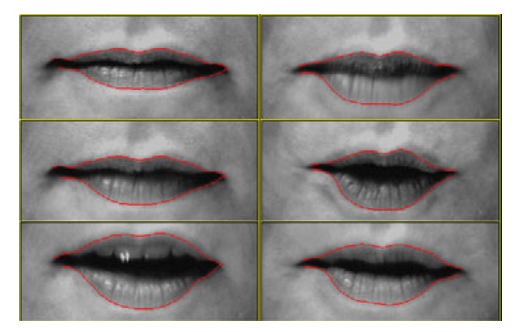
\includegraphics[scale=0.6]{img/active-cont.png}
    \caption{Esempio di applicazione dei contorni attivi: lip tracking.}
    \label{fig:lip_track}
\end{figure}

Questo tipo di algoritmo si basa su informazioni locali del gradiente dell'intensità dei pixel e le utilizza per attrarre la curva verso i bordi dell'oggetto. In particolare i bordi, essendo caratterizzati da un cambiamento improvviso dell'intensità, presentano un gradiente elevato, di conseguenza l'algoritmo cerca iterativamente di portare i punti che formano la curva in pixel con gradienti alti.
Questo meccanismo viene formalizzato con un problema di ottimizzazione, ovvero si vuole massimizzare la somma dei gradienti dell'intensità dei pixel dove sono i punti della curva.
Per quanto riguarda la definizione di un contorno, esso è definito come un insieme di punti nello spazio bidimensionale connessi da linee rette:

\begin{equation}
    V = \{v_{i} = (x_{i}, y_{i}) | i = 0,1,2,...., n-1\}.
\end{equation}

Dove $n$ è il numero dei punti che formano la curva. Come detto precedentemente, si vuole massimizzare la somma dell'intensità dei gradienti e per fare ciò viene utilizzata la magnitudine del gradiente dell'intensità dei pixel al quadrato, ovvero $||\nabla I||^{2}$. Inoltre, dato che la curva deve essere attratta dai gradienti più alti, bisogna espandere il "campo di forza" dei picchi del gradiente, altrimenti un punto non vicinissimo a un bordo non verrebbe attratto. Per fare questo utilizziamo la sfocatura gaussiana applicata alla magnitudine del gradiente e di conseguenza il valore da massimizzare diventa $||\nabla n_{\sigma} \ast I||^{2}$. Infine, il problema viene trasformato nel trovare il minimo di $E_{image}$, dove:

\begin{equation}
    E_{image} = -\sum_{i=0}^{n-1}{||\nabla n_{\sigma} \ast I(v_{i})||^{2}}.
\end{equation}

A questo punto, l'algoritmo non fa altro che cercare iterativamente di ottimizzare $E_{image}$ portando ogni punto in una nuova posizione, fino a che questo non raggiunge una certa soglia stabilita in anticipo. Il problema di questa versione è che è molto sensibile al rumore e molto spesso il contorno tende ad assumere forme strane, proprio a causa della presenza del rumore del gradiente intorno all'oggetto. 
Per superare questa difficoltà, e perché in generale si vuole una curva che rispetti alcune caratteristiche naturali, come se simulasse un oggetto fisico, come l'elasticità e la morbidezza, al problema di ottimizzazione viene aggiunto un secondo componente $E_{contour}$ che rappresenta questi vincoli di forma.
In particolare, $E_{contour}$ è composta a sua volta da altri due componenti $E_{elastic}$ e $E_{smooth}$, che rappresentano le due caratteristiche appena menzionate. In realtà, a $E_{contour}$ possono essere aggiunti altri componenti a seconda del task specifico e di come si voglia vincolare la forma della curva. Ad esempio, molto spesso quando si conosce a priori la forma dell'oggetto d'interesse, si può aggiungere al problema un componente che penalizzi forme diverse da questa. Di conseguenza, la formula di $E_{contour}$ è la seguente:

\begin{equation}
    E_{contour} = \alpha E_{elastic} + \beta E_{smooth}.
\end{equation}

Dove $\alpha$ e $\beta$ sono due coefficienti che rappresentano il peso che vogliamo dare ai due vincoli di elasticità e morbidezza.
Per quanto riguarda il vincolo di elasticità, esso rappresenta il desiderio che la curva simuli il comportamento di un elastico, ovvero quando due punti della curva sono più distanti c'è una sorta di forza di attrazione più forte e di conseguenza la curva tende a non distanziare troppo i punti tra loro. Di seguito la formula del componente di elasticità di un punto del contorno $v(s)$.

\begin{equation}
    E_{elastic}(v(s)) = \bigg|  \frac{\delta}{\delta s} v(s)  \bigg|^{2}.
\end{equation}


Ovvero il quadrato della derivata prima del punto del contorno, che rappresenta l'intuizione del fatto che non si vogliono grandi distanze da un punto all'altro. Per quanto riguarda il componete di morbidezza, invece, esso è definito come:


\begin{equation}
    E_{smooth}(v(s)) = \bigg|  \frac{\delta^{2}}{\delta^{2} s} v(s)  \bigg|^{2}.
\end{equation}

Ovvero il quadrato della derivata seconda del punto del contorno, che invece rappresenta l'intuizione del fatto che non si vogliono cambiamenti improvvisi. Dato che in realtà la curva del contorno è composta da punti discreti, le formule dei due componenti diventano:


\begin{equation}
    E_{elastic}(v(i)) = (x_{i+1} - x_{i})^{2} + (y_{i+1} - y_{i})^{2}.
\end{equation}

\begin{equation}
    E_{smooth}(v(i)) = (x_{i+1} -  2x_{i} + x_{i-1})^{2} + (y_{i+1} -  2y_{i} + y_{i-1})^{2}.
\end{equation}

e quindi

\begin{equation}
    E_{elastic} = \sum_{i=0}^{n-1}{(x_{i+1} - x_{i})^{2} + (y_{i+1} - y_{i})^{2}}.
\end{equation}

\begin{equation}
    E_{smooth} = \sum_{i=0}^{n-1}{(x_{i+1} -  2x_{i} + x_{i-1})^{2} + (y_{i+1} -  2y_{i} + y_{i-1})^{2}}.
\end{equation}


Infine, il problema totale diventa minimizzare il seguente valore:

\begin{equation}
    E_{total} = E_{image} + E_{contour}.
\end{equation}

La Figura \ref{fig:coin-contour} illustra un esempio di come il risultato migliori aggiungendo il componente $E_{contour}$.
\\
\begin{figure}[h!]
    \centering
    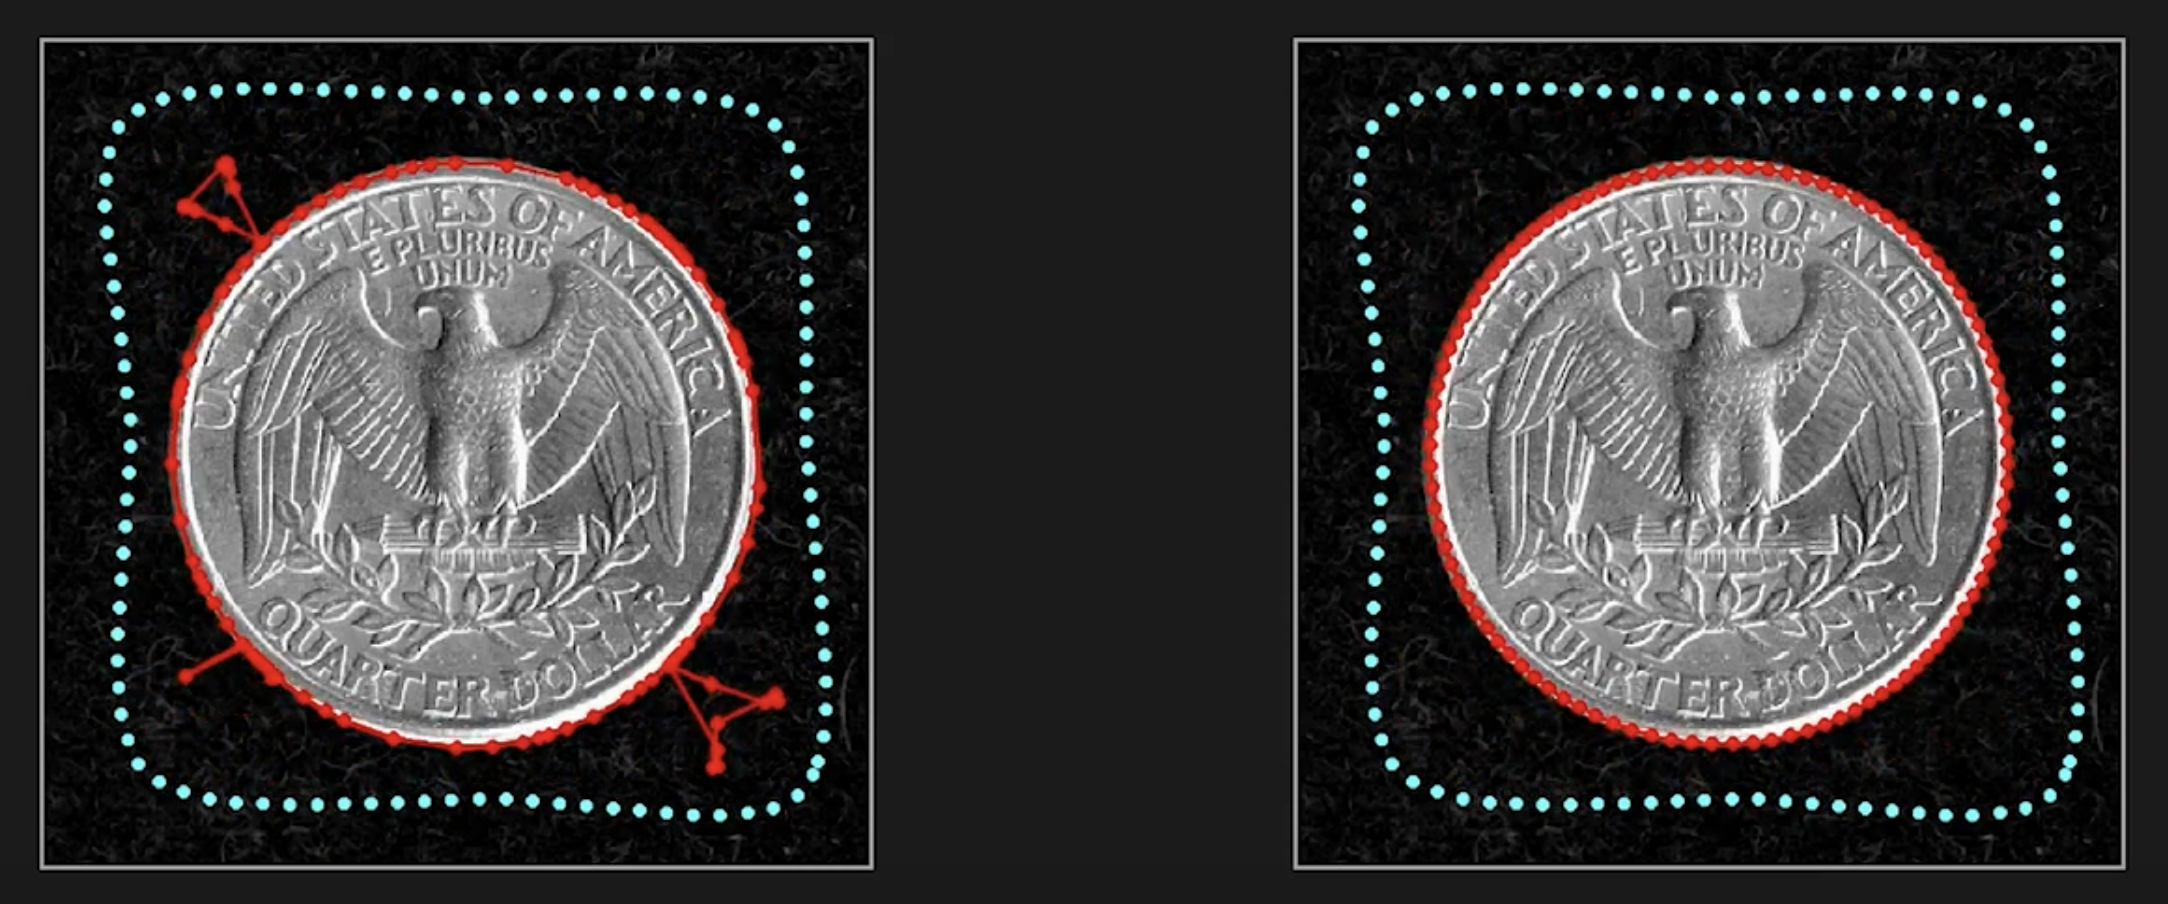
\includegraphics[scale=0.35]{img/activ_cont3.png}
    \caption{Esempio di applicazione del metodo del contorno attivo. In entrambe le immagini possiamo vedere un contorno blu (contorno di inizializzazione) e uno rosso (contorno finale). In particolare, a sinistra è stata utilizzata la versione dell'algoritmo che minimizza $E_{image}$, mentre a destra viene minizzato $E_{total}$ e possiamo notare come quello a destra ottenga un risultato migliore.}
    \label{fig:coin-contour}
\end{figure}

Come già anticipato, le performance di questo algoritmo dipendono molto dalla bontà dell'inizializzazione, inoltre performa bene soprattutto con immagini che contengono un solo oggetto, anche se si può utilizzare su immagini che ne contengono più di uno. In particolare, a seconda della natura degli oggetti si possono variare i parametri $\alpha$ e $\beta$, per dar modo al contorno di adattarsi meglio  agli oggetti (Figura \ref{fig:two-coin-segm}). In altri casi, come già menzionato, può risultare utile aggiungere ulteriori componenti a $E_{contour}$ oltre a $E_{elastic}$ e $E_{smooth}$.
Infine, esiste una variante dell'algoritmo che, invece di far partire il contorno da una forma più larga per poi farlo contrarre sull'oggetto, fa partire il contorno dal suo interno e lo fa gonfiare fino a modellare i suoi bordi.

\begin{figure}
     \centering
     \begin{subfigure}[b]{0.6\textwidth}
         \centering
         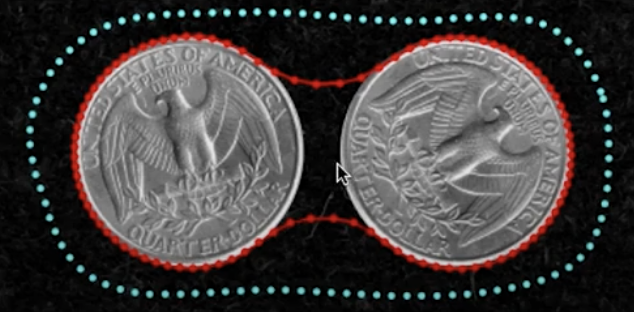
\includegraphics[width=\textwidth]{img/activ_cont4.png}
         \caption{$\alpha$ piccolo}
         \label{fig:y equals x}
     \end{subfigure}
     \hfill
     \begin{subfigure}[b]{0.6\textwidth}
         \centering
         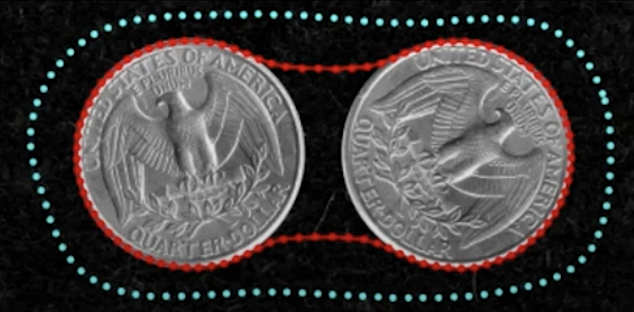
\includegraphics[width=\textwidth]{img/activ_cont5.png}
         \caption{$\alpha$ grande}
         \label{fig:three sin x}
     \end{subfigure}
        \caption{Esempio di segmentazione di due oggetti con un contorno attivo, variando però il coefficiente $\alpha$. Come si può notare, abbassando $\alpha$ si dà modo al contorno di adattarsi meglio ai due oggetti. Chiaramente, come modificare i due coefficienti $\alpha$ e $\beta$ dipende dalla natura dell'immagine.}
        \label{fig:two-coin-segm}
\end{figure}











\subsection{Metodi di clustering}
\label{metodi_clustering}
Così come i metodi basati su grafi hanno trasformato l'immagine in un grafo facendo corrispondere a ogni pixel un nodo, allo stesso modo i metodi di clustering trasformano l'immagine in una distribuzione in uno spazio euclideo a più dimensioni. In particolare, la prima fase di un metodo di questa categoria è capire su quali feature basarsi per mappare ogni pixel in un punto dello spazio. Una delle scelte più semplici, nel caso di immagini RGB, è quella di utilizzare i tre canali dell'immagine, ovvero la quantità di rosso, di verde e di blu (Figura \ref{fig:scimmia}). Altre feature molto utilizzate sono la luminosità, la posizione del pixel, la profondità (RGB-D), ma anche feature più complesse come la texture. Ancora una volta, la scelta di queste feature è molto importante, ma soprattutto dipende fortemente dal campo di applicazione e dalla natura delle immagini, di conseguenza è necessaria un'approfondita conoscenza di entrambi.

\begin{figure}[h!]
     \centering
     \begin{subfigure}[b]{0.4\textwidth}
         \centering
         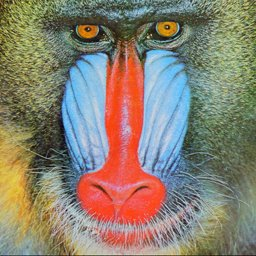
\includegraphics[width=\textwidth]{img/scimmia.jpeg}
         \caption{}
         \label{fig:y equals x}
     \end{subfigure}
     \hfill
     \begin{subfigure}[b]{0.5\textwidth}
         \centering
         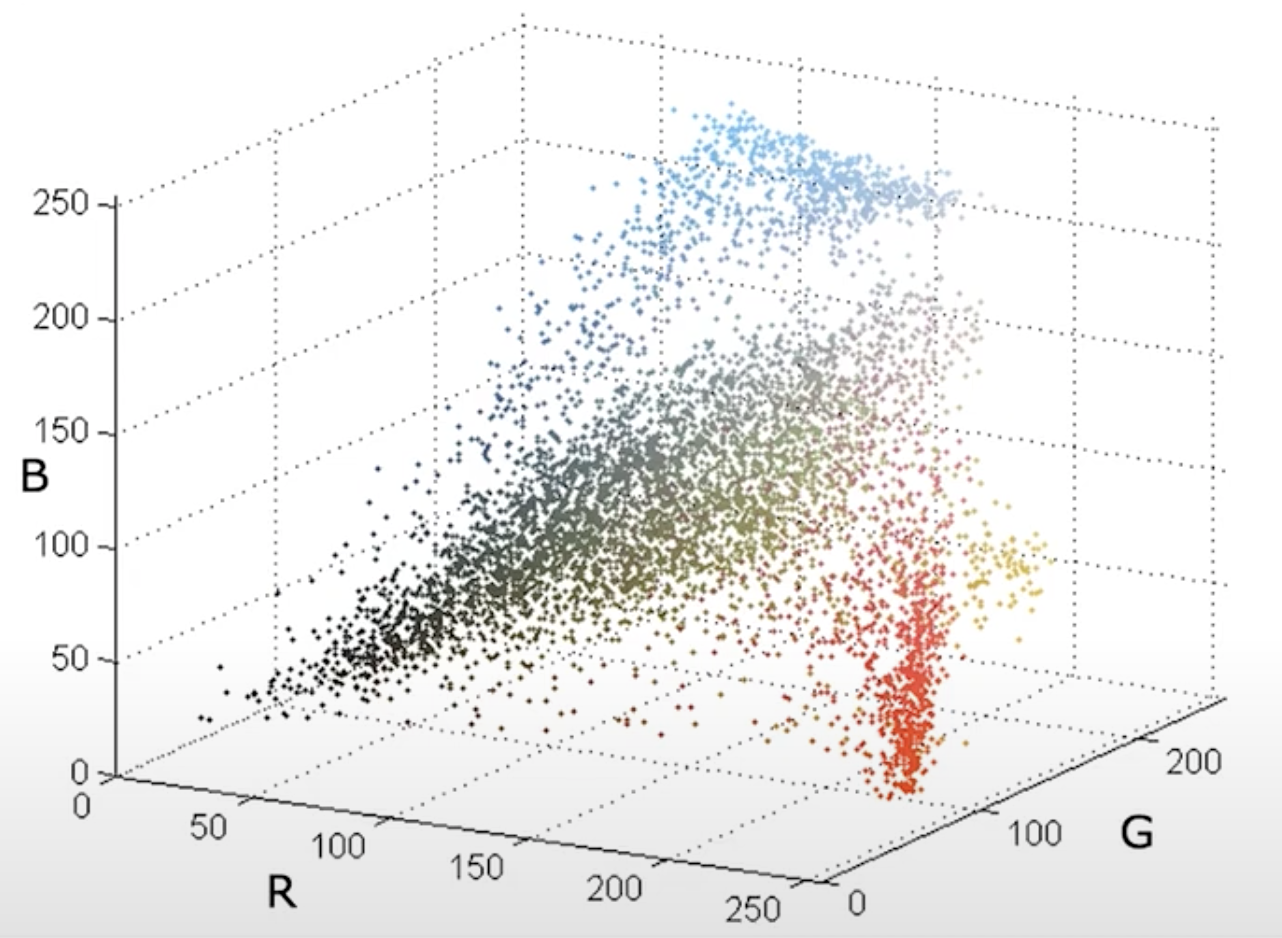
\includegraphics[width=\textwidth]{img/plot-scimmia.png}
         \caption{}
         \label{fig:three sin x}
     \end{subfigure}
        \caption{Le due figure sono un esempio di come un'immagine (a) si possa mappare in un spazio tridimensionale (b) utilizzando come feature i tre canali dell'immagine (RGB).}
        \label{fig:scimmia}
\end{figure}

Una volta completata la mappatura dell'immagine nello spazio scelto, ogni pixel $i$ viene rappresentato con un vettore di feature $f_{i}=[f_{i}^1, f_{i}^2, f_{i}^3, ..., f_{i}^k]$ dove $k$ è il numero di feature scelte. Così come in altri metodi, per guidare l'algoritmo nel raggruppare i pixel, viene utilizzata una misura della loro similarità . In particolare, la similarità viene rappresentata dalla distanza nello spazio dei vettori di feature dei pixel e per calcolarla viene utilizzata quella che è chiamata distanza $L^2$ o distanza euclidea, definita in uno spazio a $k$ dimensioni come:

\begin{equation}
    S(f_{i}, f_{j}) = \sqrt{\sum_{k}{(f_{i}^k-f_{j}^k)^2}}.
\end{equation}

A questo punto, il task della segmentazione è stato totalmente trasformato in un problema di clustering (Figura \ref{fig:scimmia2}) e può essere utilizzato un qualsiasi algoritmo che risolva questo tipo di problema. Di algoritmi che risolvono questo tipo di problema ne esistono diversi, tra i più noti ci sono K-Means e Mean Shift.


\begin{figure}[h!]
     \centering
     \begin{subfigure}[b]{0.4\textwidth}
         \centering
         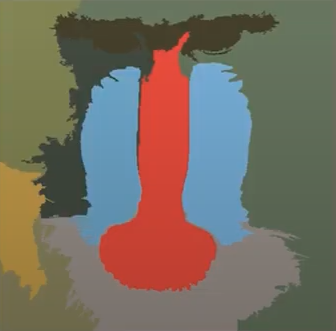
\includegraphics[width=\textwidth]{img/scimmia2.png}
         \caption{}
         \label{fig:y equals x}
     \end{subfigure}
     \hfill
     \begin{subfigure}[b]{0.5\textwidth}
         \centering
         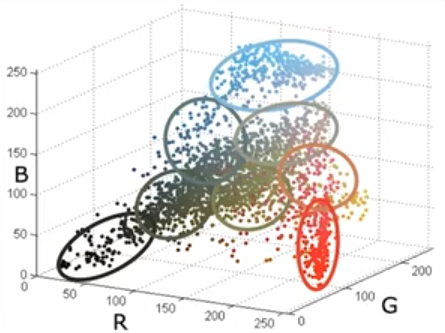
\includegraphics[width=\textwidth]{img/plot-scimmia2.png}
         \caption{}
         \label{fig:three sin x}
     \end{subfigure}
        \caption{Le due immagini mostrano il risultato di un algoritmo di clustering applicato alla mappatura dell'immagine della Figura \ref{fig:scimmia}a. Nella (a) il risultato finale, ovvero l'immagine segmentata; la (b) invece mostra il clusters nello spazio tridimensionale.}
        \label{fig:scimmia2}
\end{figure}




\subsubsection{K-means}
Probabilmente, l'algoritmo di clustering più noto è il \textit{k-means} \cite{lloyd1982least, macqueen1967some}. Il suo funzionamento è abbastanza semplice e si basa sull'obiettivo di trovare il centroide o punto medio, di ogni cluster, ovvero trovare il punto che minimizzi la varianza totale intra-gruppo $Var$, che non è altro che una misura della variabilità all'interno del cluster. Formalmente, il problema è definito come trovare:

\begin{equation}
    \underset{S}{\arg\min} \sum_{i=1}^{k}{|S_{i}| Var(S_{i})}.
\end{equation}

Dove $S={S_{1},S_{2},..., S_{k}}$ è l'insieme dei cluster. Una volta trovati i centroidi di ogni cluster, il cui numero $k$ deve essere definito in anticipo, l'algoritmo classifica ogni punto nello spazio determinando quale dei $k$ centroidi sia il più vicino. Per quanto riguarda la prima fase della ricerca dei centroidi, l'algoritmo parte inizializzando $k$ centroidi e calcolando i cluster secondo la regola del centroide più vicino. A questo punto, l'algoritmo ripete iterativamente questo meccanismo, ricalcolando ogni volta i centroidi dei cluster fino a non convergere, ovvero fino a che i centroidi non cambiano più posizione o comunque il loro cambiamento è sotto una certa soglia.
Ancora una volta purtroppo, le performance di questo algoritmo dipendono fortemente dalla bontà dell'inizializzazione. In questo caso, l'inizializzazione può essere fatta in diverse maniere: la cosa più semplice è quella di inizializzarli randomicamente, ma chiaramente è anche la scelta meno peformante; un altro metodo molto semplice consiste nell'inizializzarli randomicamente, controllando però che nessuno dei centroidi sia molto vicino e in quel caso reinizializzarli; un terzo metodo è quello di scegliere dei centroidi che siano uniformemente distribuiti nello spazio; infine, un ultimo metodo può essere utilizzare il k-means prima su una sottoporzione della distribuzione, e poi utilizzare i centroidi risultanti come inizializzazione per applicare l'algoritmo a tutta la distribuzione.

\begin{figure}[h!]
     \centering
     \begin{subfigure}[b]{0.4\textwidth}
         \centering
         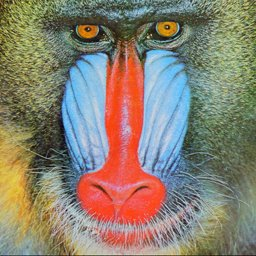
\includegraphics[width=\textwidth]{img/scimmia.jpeg}
         \caption{}
         \label{}
     \end{subfigure}
     \hfill
     \begin{subfigure}[b]{0.4\textwidth}
         \centering
         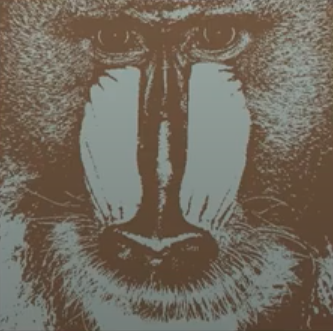
\includegraphics[width=\textwidth]{img/scimmia_k=2.png}
         \caption{}
         \label{}
     \end{subfigure}
     \hfill
     \begin{subfigure}[b]{0.4\textwidth}
         \centering
         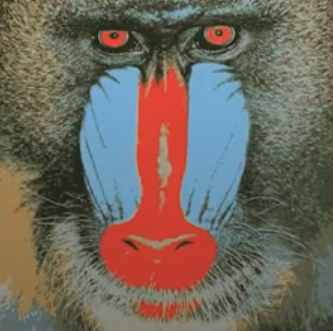
\includegraphics[width=\textwidth]{img/scimmia_k=8.png}
         \caption{}
         \label{}
     \end{subfigure}
     \hfill
     \begin{subfigure}[b]{0.45\textwidth}
         \centering
         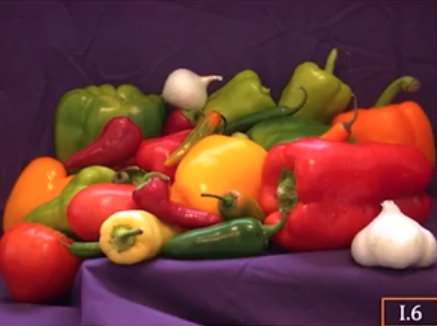
\includegraphics[width=\textwidth]{img/frutta.png}
         \caption{}
         \label{}
     \end{subfigure}
     \hfill
     \begin{subfigure}[b]{0.45\textwidth}
         \centering
         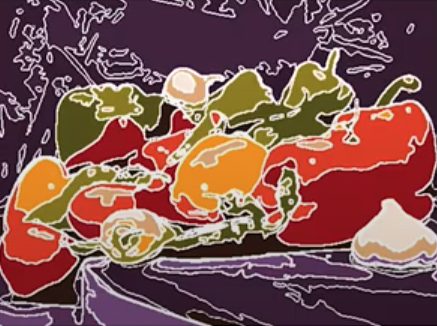
\includegraphics[width=\textwidth]{img/frutta_k=16.png}
         \caption{}
         \label{}
     \end{subfigure}
     \hfill
     \begin{subfigure}[b]{0.45\textwidth}
         \centering
         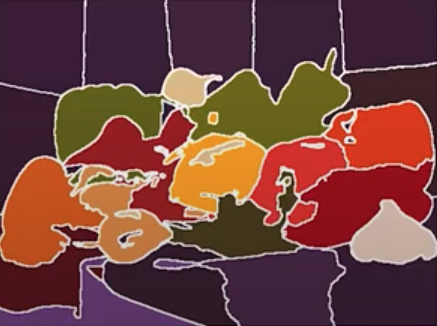
\includegraphics[width=\textwidth]{img/frutta_k=16_xy.png}
         \caption{}
         \label{fig:three sin x}
     \end{subfigure}
        \caption{Le quattro immagini mostrano il risultato dell'algoritmo k-means applicato a immagini RGB: (a) e (d) sono le due imagini originali; (b) mostra il risultato con $k=2$; (c) con $k=8$; (e) è il risultato con $k=16$ e infine (f) è il risultato con $k=16$ ma in uno spazio a cinque dimensioni ovvero $(R,G,B,x,y)$ dove $x$ e $y$ rappresentano le coordinate dei pixel nell'immagine, mentre per tutte le altre è stato utilizzato uno spazio a tre dimensioni ovvero $(R,G,B)$.}
        \label{fig:scimmia_frutta}
\end{figure}






\subsubsection{Mean Shift}
Come detto nel paragrafo precedente, l'algoritmo k-mean ha lo svantaggio di essere molto sensibile rispetto all'inizializzazione dei centroidi. Inoltre, un altro svantaggio del k-mean è che l'utente deve decidere a priori il numero di cluster. L'algoritmo \textit{mean shift} \cite{fukunaga1975estimation, comaniciu_mean} cerca di mitigare questi due problemi. Anche mean shift è un algoritmo iterativo e in particolare, il meccanismo generale si basa sul trovare le mode della distribuzione dei punti nello spazio, che ad alto livello possono essere pensate come i punti dove la distribuzione è più densa. Il funzionamento dell'algoritmo è il seguente: per ogni punto seleziona intorno a questo una finestra di dimensione $W$, che è l'unico parametro dell'algoritmo, e successivamente calcola la moda della distribuzione dei punti all'interno di quella finestra, che sarà il centro della finestra all'iterazione successiva. Ripetendo questo meccanismo finché il vettore di spostamento della moda, ovvero la distanza della moda di un' iterazione a quella dell'iterazione successiva, non si azzeri oppure non scenda sotto una certa soglia, l'algoritmo trova la moda verso la quale il punto di partenza è stato "attratto". Infine, il mean shift crea i cluster trovando i "bacini di attrazione", ovvero gli insiemi di punti che vengono attratti verso la stessa moda. La Figura \ref{fig:scimmia_frutta} mostra alcuni esempi dell'applicazione del mean shift.




\subsection{Algoritmi Supervised}
In generale, come già menzionato, una volta mappata l'immagine in uno spazio multidimensionale di feature, il task della segmentazione si può ricondurre, nel caso in cui il numero di classi fosse noto a priori, in un classico task di classificazione Machine Learning. Di conseguenza, tutti gli algoritmi  di Machine Learning per la classificazione diventano validi per risolvere il problema della segmentazione. Di algoritmi di classificazione ne esistono svariati e tra i più popolari vi sono l'SVM (Support Vector Machines), il Regressore logistico, alberi decisionali, K-nearest neighbor e molti altri. La principale differenza con gli algoritmi menzionati nei paragrafi precedenti (\ref{metodi_soglia}, \ref{metodi_dividi_fondi}, \ref{metodi_grafi}, \ref{metodi_contorni}, \ref{metodi_clustering}) è che questi ultimi rientrano nella categoria di algoritmi unsupervised, mentre tutti i classificatori di Machine Learning appena menzionati rientrano in quella supervised, ovvero hanno bisogno di un dataset per poter apprendere i propri parametri e riuscire a classificare.

%\subsubsection{Support Vector Machines}
%FORSE DA TOGLIERE

%L'SVM è un algoritmo di classificazione il cui obiettivo è quello di costruire un classificatore binario lineare che riesca a separare l'insieme di punti, che gli sono stati forniti sotto forma di dataset, nelle due classi. Il classificatore lineare che viene costruito è definito dalla seguente equazione:

%\begin{equation}
%    y=W^{T}X+b.
%\end{equation}

%dove $W$ e $b$ sono i parametri del classificatori che vengono appresi durante algoritmo, $X$ è il vettore in input e $y$ rappresenta il valore con cui il classificatore deciderà la label di $X$. L'idea generale dietro l'SVM è quella di costruire un iperpiano di forma

%\begin{equation}
%    W^{T}X+b=0.
%\end{equation}

%che massimizzi la sua distanza dai punti del dataset rimanendo però coerente con il dataset, ovvero che clasifici bene i suoi punti. in particolare, per quanto riguarda questa distanza, durante le iterazioni alcuni punti, chiamati vettori di supporto (\textit{support vectors}, da cui il nome) assumono un'importanza più elevata perché i più vicini al iperpiano. In particolare, questa distanza rappresenta la distanza tra l'iperpiano del classificatore, anche chiamato confine di decisione, e i due iperpiani paralleli che intersecano i vettori di supporto delle due classi.




\section{Approcci di Deep Learning}
Oltre agli approcci classici, vi sono tecniche di Deep Learning che utilizzano architetture complesse, per riuscire ad apprendere il pattern d'interesse e in particolare, per apprendere le feature che determinano la semantica dei pixel, cosa che invece deve essere fatta manualmente quando si utilizzano gli algoritmi di Machine Learning (fase della \textit{feature extraction}).\\

%\subsection{Architetture di Deep Learning}

 
 \subsection{Architetture basate sul contesto}
 \label{context_based}
Questa categoria di architetture utilizza una tipologia di informazione molto importante e che i metodi di cui abbiamo parlato nei capitoli precedenti non utilizzano, ovvero il contesto di un pixel. In particolare, il contesto risulta molto importante per la classificazione semantica di un pixel, in quanto spesso le feature locali di un pixel come il colore, la luminosità, ma anche altre più complesse, non sono sufficienti per distinguere due pixel di classi diverse. Come già visto, in generale nel campo della Computer Vision la tipolgia di architettura più utilizzata è la CNN, che si basa sulle presenza di strati convoluzioni, ed è proprio grazie a questi che l'architettura riesce ad estrapolare il contesto di un pixel. In particolare, la categoria delle architetture context-based fa un forte uso delle convoluzioni in diverse forme. Una delle varianti più utilizzate per catturare un contesto più ampio del pixel, senza però andare ad aumentare di troppo il costo computazionale, è la convoluzione dilatata. In particolare alcune, per fare in modo di costruire campi ricettivi con diverse ampiezze, fanno uso delle convoluzioni dilatate a diverse scale. Ad esempio, la DilatedNet \cite{yu2015multi} fa uso di cinque diversi parametri di dilatazione, ovvero 1,2,4,8 e 16, ottendeno una mIoU del 67.6\% sul dataset PASCAL VOC 2012. In \cite{parsenet} le feature locali di un pixel vengono fuse con le feature globali dell'immagine, così facendo aggiungono al contesto locale del pixel quello globale, ottenendo una mIoU di 69.8\% sul PASCAL VOC 2012. In \cite{pspnet} invece, viene utilizzato un modulo chiamato \textit{Pyramid Pooling Module} (PPM), che utilizza uno strato di pooling a diverse scale per poi fondere i risultati di questi pooling insieme, in modo da avere informazioni di contesto a diverse scale (Figura \ref{fig:PPM}). In particolare, l'idea è che con il solo utilizzo del contesto globale, si ha una perdita di informazioni nelle sotto regioni, mentre utilizzando il PPM vengono catturate le informazioni a diverse scale, compresa quella globale. Il PPM ha poi ispirato moltri altri lavori che, apportando modifiche, hanno migliorato ancora di più le performance, come ad esempio la DeepLabV2 \cite{deeplabv2}, che  a partire dall'idea del PPM ha costruito il modulo Atrous Spatial Pyramid Pooling (ASPP), sostituendo in sostanza la normale convoluzione e il pooling con la convoluzione dilatata a diverse scale, ovvero con diverse dilatazioni, ottenendo su PASCAL VOC una mIoU di 79.7\%.

\begin{figure}[h!]
    \centering
    \hspace*{-0.1in}
    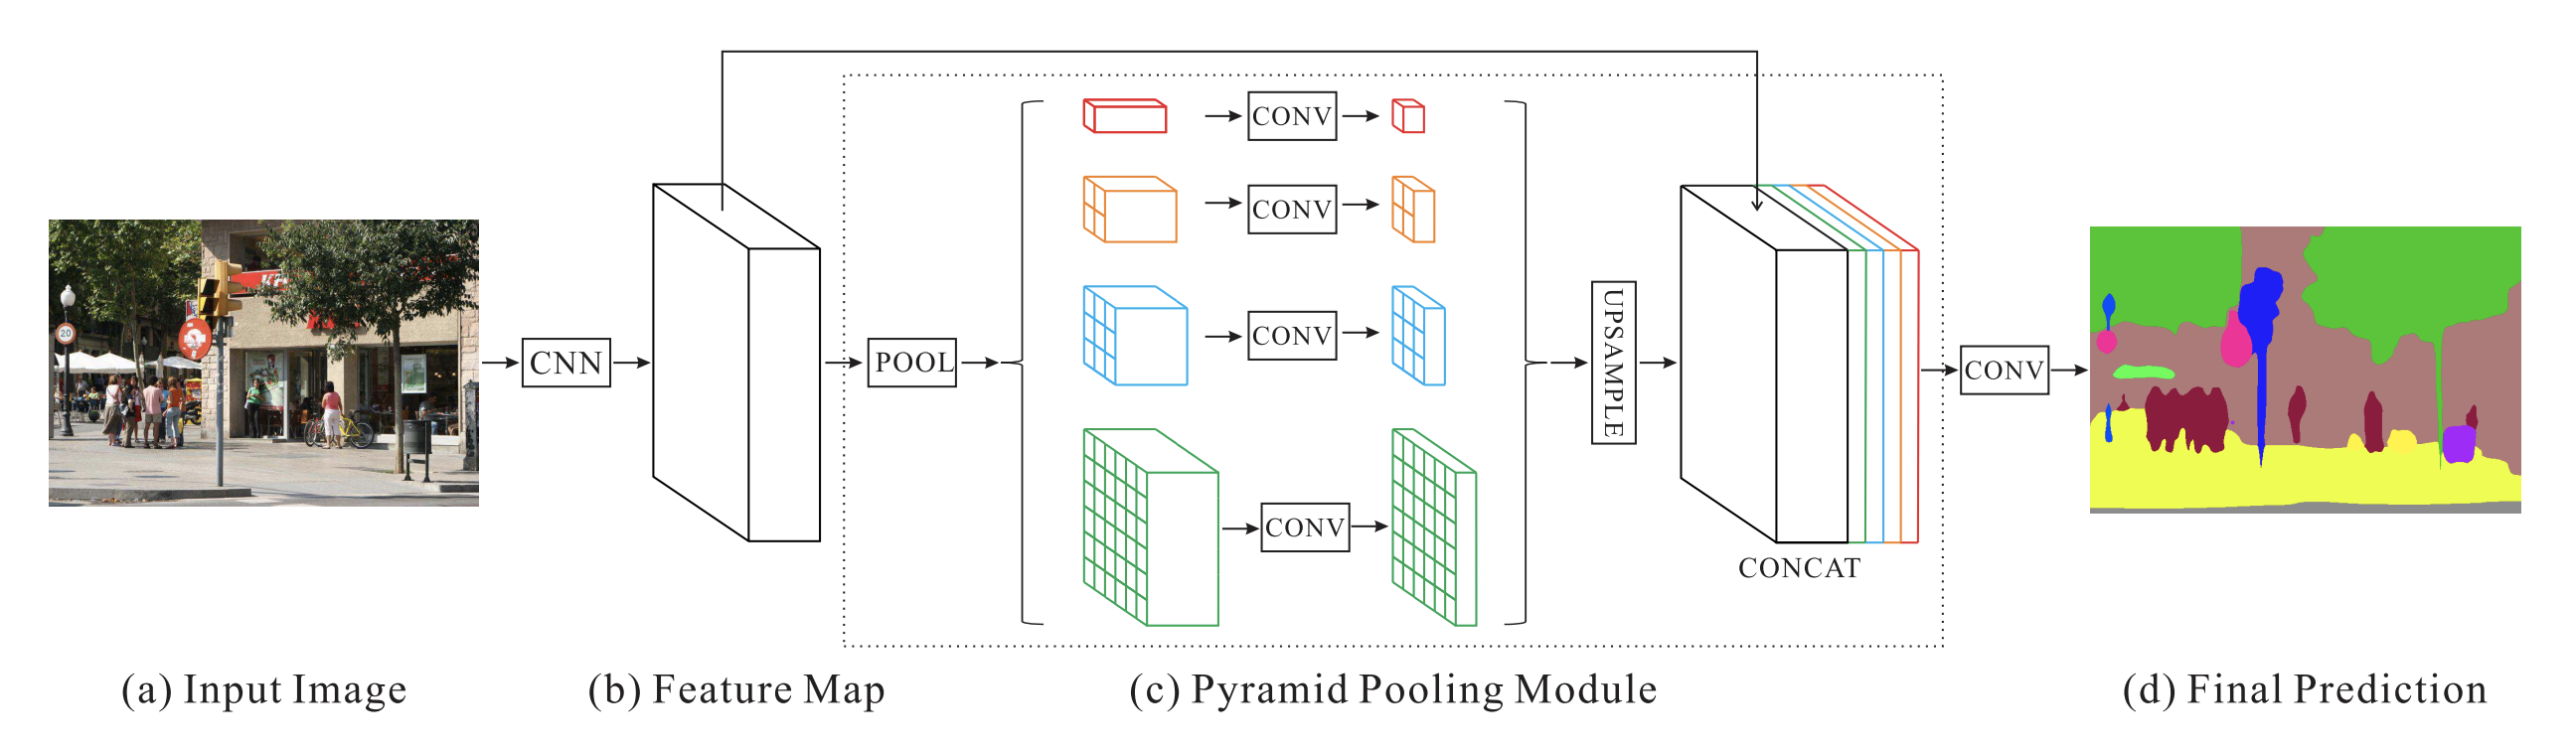
\includegraphics[scale=0.3]{img/PPM.png}
    \caption{Illustrazione del Pyramid Pooling Module (PPM) \cite{pspnet}.}
    \label{fig:PPM}
\end{figure}




 
 \subsection{Architetture basate sul feature-enhacement}
Il concetto generale alla base di questa categoria di architettura è che, nelle CNN, l'estrazione strato per strato di feature sempre più di alto livello causa una perdita di informazioni spaziali. In particolare, a causa soprattutto del pooling e delle convoluzioni con stride, le feature avanzando progressivamente nella rete, diminuiscono di risoluzione e di conseguenza perdono le informazioni spaziali, che in task come la classificazione non sono importanti, ma che invece lo sono nel task della segmentazione. La soluzione proposta da questa categoria di architetture per risolvere questo problema è unire i due aspetti, ovvero unire le feature dei primi livelli, che hanno soprattutto informazioni spaziali, con quelle dei livelli più profondi, che invece non hanno molta informazione spaziale ma contengono informazioni sulle feature di alto livello. Una delle prime architteture di questo tipo è stata la FCN \cite{FCNs}, che mette in atto questa idea aggiungendo delle \textit{skip connections}, collegando così le feature degli strati intermedi con quelle degli ultimi strati. La UNet \cite{unet} è un'altra architettura che si rifà a questo concetto ed è una delle architetture più note nel campo della segmentazione semantica. In particolare, la UNet, chiamata così per la sua peculiare forma a U, a differenza della FCN utilizza delle skip connections tra tutti gli strati, ovvero connette tutte le feature della prima parte della rete, responsabile della feature extraction e chiamata encoder, a quelle della seconda parte della rete, chiamata decoder (Figura \ref{fig:unet}).
 
 \begin{figure}[h!]
    \centering
    \hspace*{0.1in}
    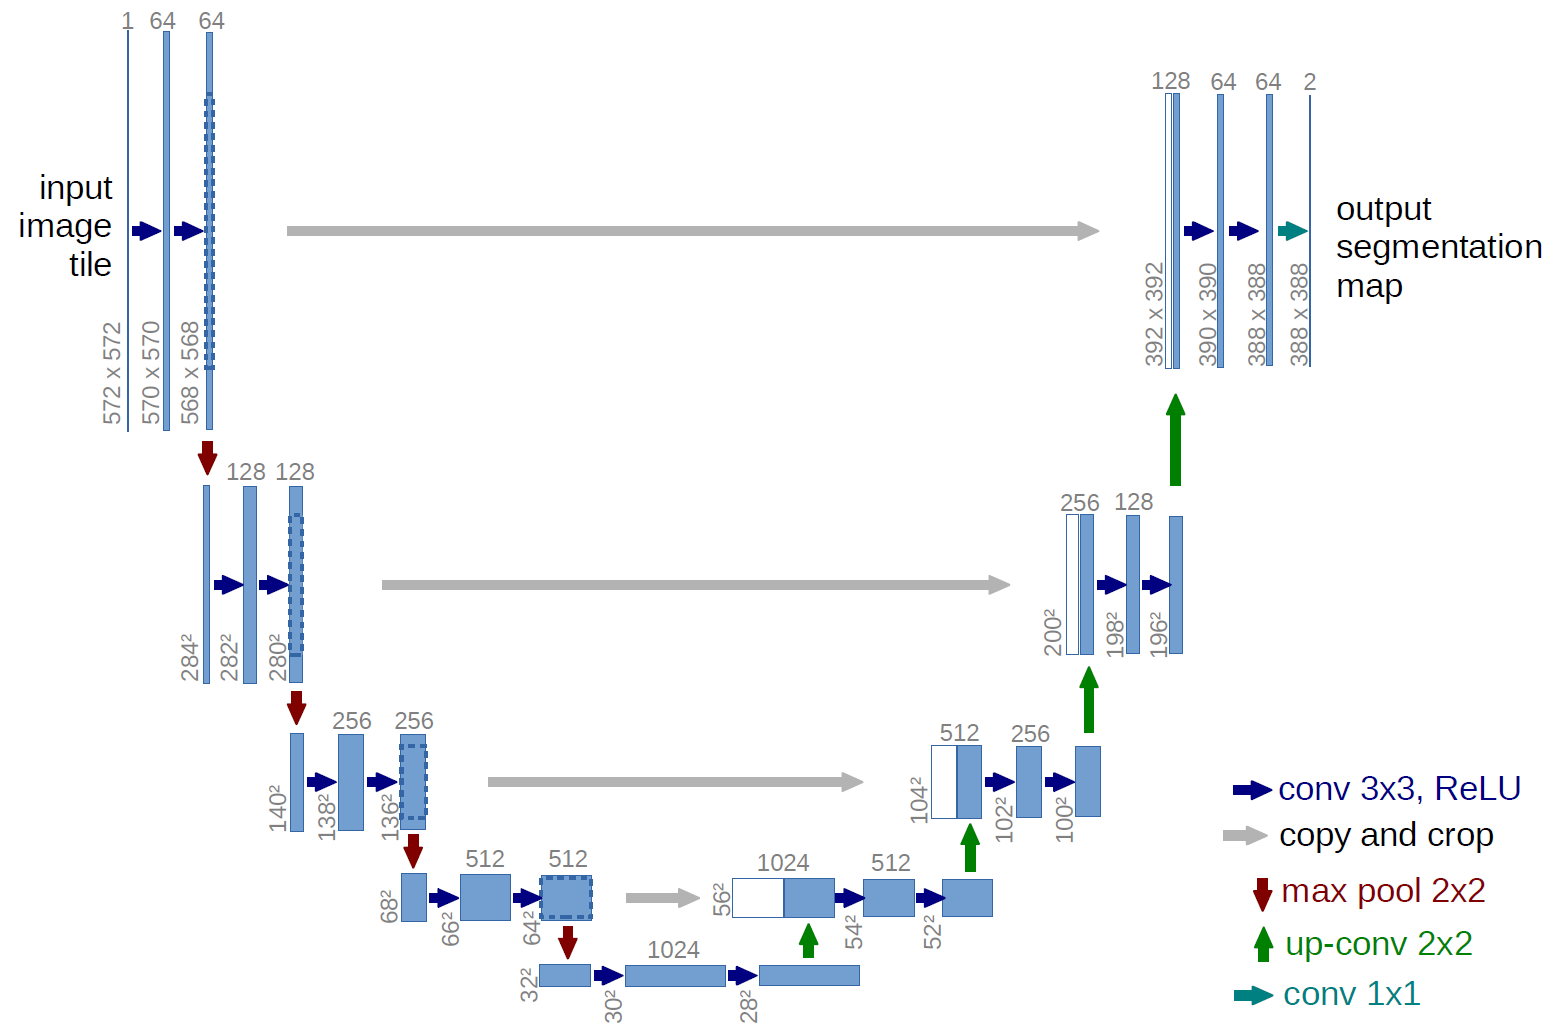
\includegraphics[scale=0.22]{img/unet.png}
    \caption{Architettura della UNet \cite{unet}.}
    \label{fig:unet}
\end{figure}
 
 
\subsection{Architetture basate sulla deconvoluzione}
La prima architettura di questo tipo è stata la DeconvNet \cite{deconvnet}, che ha una struttura encoder-decoder. In particolare, questa rete utilizza, a parte i classici moduli di pooling, convoluzione, e via dicendo, altre due tipologie di modulo, ovvero l'unpooling e la deconvoluzione. L'idea alla base del loro utilizzo è far fronte al problema della perdita di precisione nelle informazioni spaziali, nella parte di decoder in cui viene fatto l'upsample delle feature map per riportarle alla risoluzione originale. In particolare, negli strati di pooling dell'encoder, viene memorizzato l'indice della cella più grande, in modo che, nella fase di upsample, il modulo di unpooling possa ricreare la stessa finestra che era passata dentro lo strato di pooling. L'output dell'unpooling, tuttavia, ha delle celle azzerate, questo poiché nel corrispettivo pooling nell'encoder viene memorizzata soltanto la cella maggiore, ma non le altre. Per risolvere questo problema l'output del modulo di unpooling viene passato alla deconvoluzione che, grazie ai parametri appresi, riesce a ricostruire la feature map (Figura \ref{fig:deconv}).
 
\begin{figure}[h!]
    \centering
    \hspace*{0.1in}
    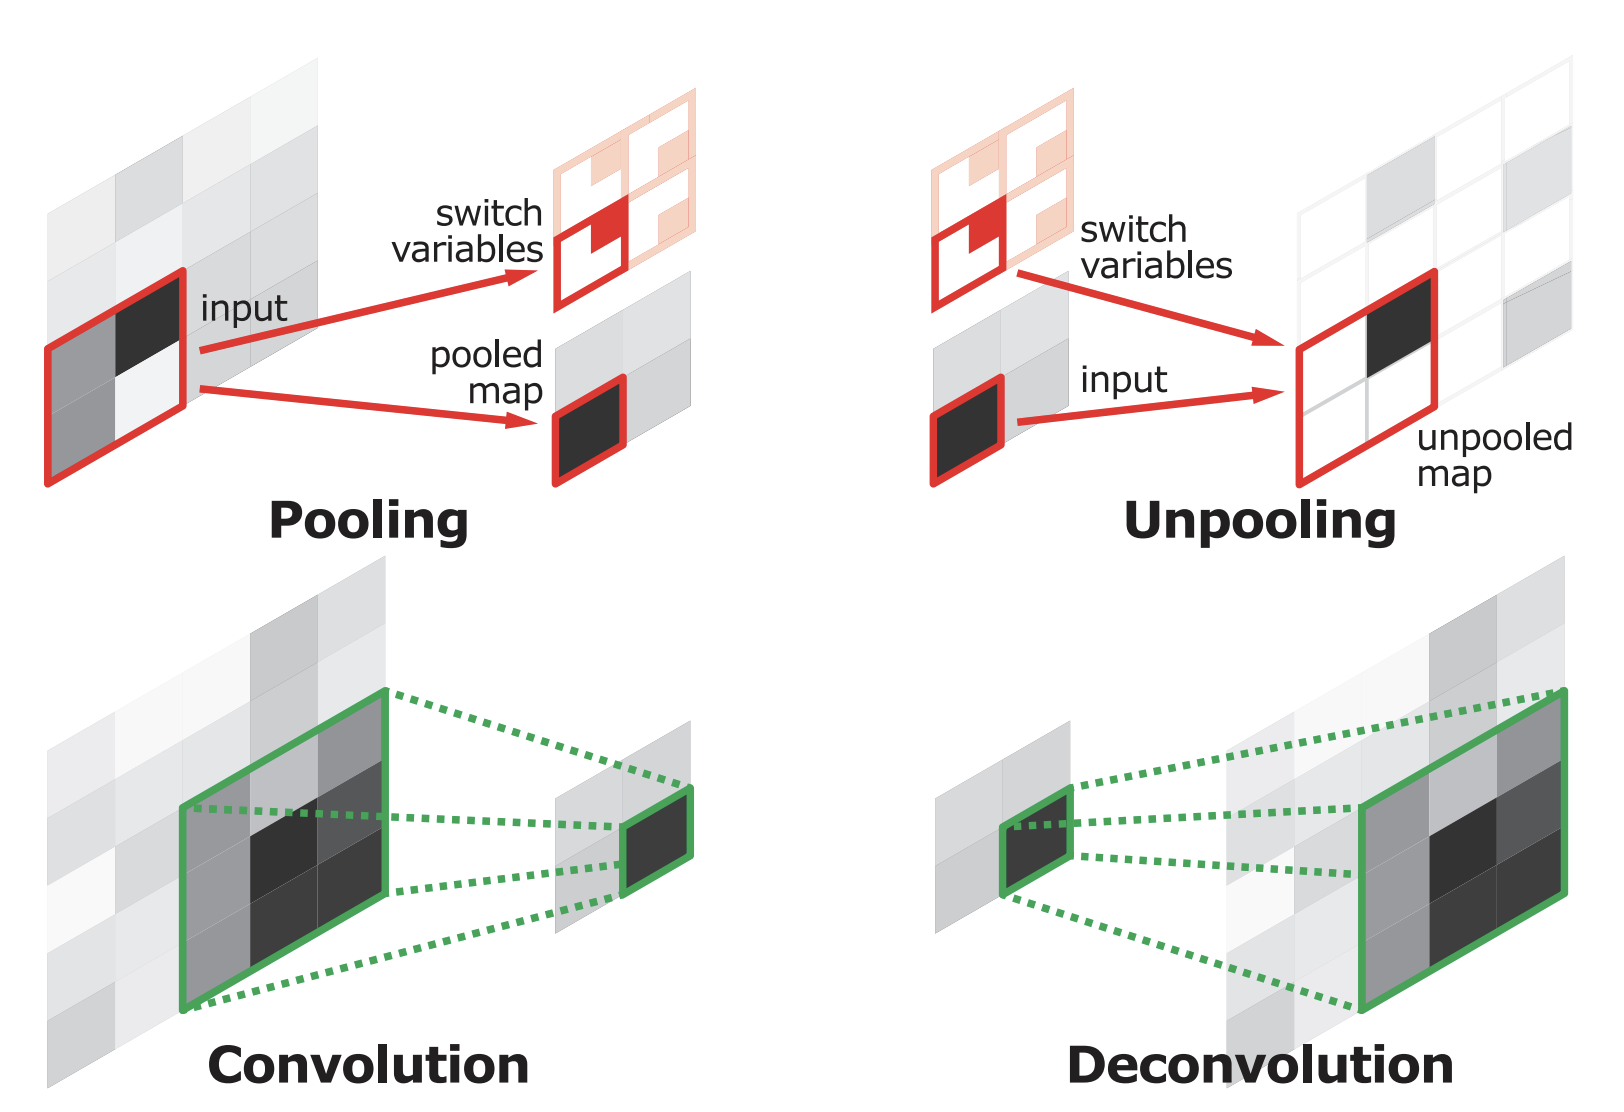
\includegraphics[scale=0.35]{img/deconv.png}
    \caption{Illustrazione dei due moduli di unpooling e di deconvoluzione \cite{deconvnet} e della loro differenza con, rispettivamente, il pooling e la convoluzione.}
    \label{fig:deconv}
\end{figure}
 
 

 
\subsection{Architetture basate sulle GAN}
Questa tipologia di architettura è composta da due reti chiamate "segmentatore" e "rete avversaria" (\textit{adversarial network}). La prima ha la responsabilità, partendo dall'immagine in input, di crearne una partizione in sotto-regioni non intersecanti, ovvero la maschera. La seconda, invece, ha la responsabilità di distinguere tra l'output della prima rete e la maschera corretta. In particolare, le due reti sono messe una contro l'altra: il segmentatore ha l'obiettivo di non far capire alla seconda rete la differenza tra il suo output e la vera maschera, mentre la seconda rete (Figura \ref{fig:anet}) ha l'obiettivo di capire la differenza. L'ANet \cite{anet} è una delle prime reti di questo tipo utilizzate per la segmentazione semantica e in particolare, il concetto principale alla sua base è che la rete avversaria, a differenza di una classica loss function utilizzata per l'addestramento di una rete, riesce a cogliere differenze di più alto livello tra l'output del segmentatore e la maschera, come ad esempio differenze nella forma degli oggetti o nelle loro proporzioni. La prima rete, quella responsabile della segmentazione, utilizza per l'addestramento una loss function composta, ovvero la loss function finale è il risultato della somma pesata di due ulteriori loss function, una classica cross entropy e un'adversarial loss function. In particolare, la seconda loss function rappresenta quanto la rete avversaria riesca a distinguere tra il suo output e la maschera corretta.
 

\begin{figure}[h!]
    \centering
    \hspace*{0in}
    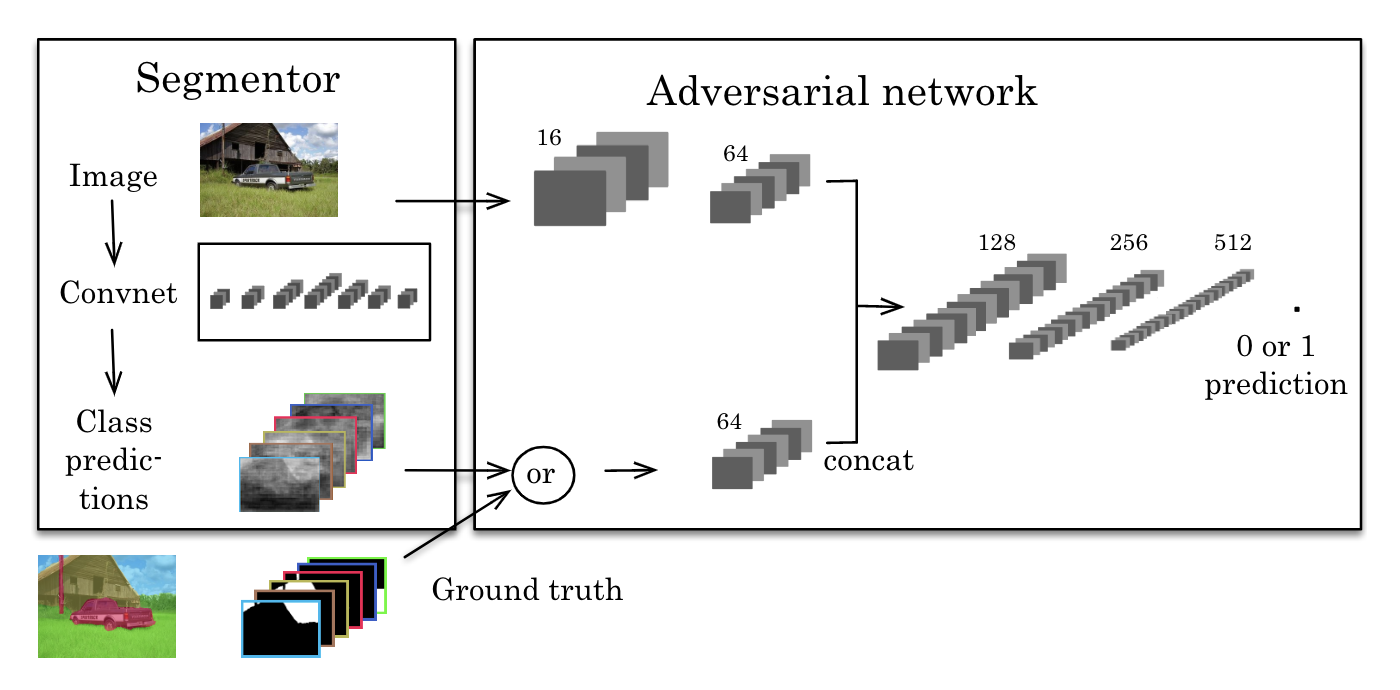
\includegraphics[scale=0.55]{img/gan.png}
    \caption{Panoramica dell'architettura basata sulle GAN proposta in \cite{anet}. A sinistra il segmentatore prende l'immagine RGB come input, e produce la maschera. A destra la rete avversaria prende la maschera prodotta dal segmentatore e produce una label (1 = maschera corretta, o 0 = maschera sintetica del segmentatore). La rete avversaria opzionalmente può prendere anche l'immagine RGB come input.}
    \label{fig:anet}
\end{figure}


\chapter{Deep Learning}
\label{deep_learning}
Il Machine Learning (ML) è una branca dell’Intelligenza Artificiale (IA) che si occupa di costruire modelli che apprendono dai dati che gli vengono forniti. Il Deep Learning, a sua volta, è una branca del ML e anch’esso si occupa di costruire modelli che apprendono pattern dai dati. La peculiarità del DL sta nella tipologia di modelli utilizzati, ovvero le reti neurali, anche dette Artifical Neural Networks (ANN) o Deep Neural Network (DNN). Una ANN è un modello di calcolo ispirato alla struttura delle reti neurali del cervello, ed è costituita da un gran numero di componenti di calcolo di base (neuroni), che sono collegati tra loro in una rete di comunicazione complessa attraverso la quale è in grado di approssimare funzioni molto complesse.
L’utilizzo delle reti neurali infatti, diventa fondamentale quando il pattern che si cerca di apprendere è molto complesso e soprattutto non lineare. Proprio questa capacità di apprendere pattern complessi ha reso il DL un tool molto utilizzato e che ha portato netti miglioramenti in molti campi, tra cui il Natural Language Processing, speech recognition, campo medico, sistemi di trasporto intelligenti \cite{dlsurvey} e molti altri \cite{dlsurvey2}. La Figura \ref{fig:appl_dl} illustra diversi campi di applicazione del DL.
\begin{figure}[h!]
    \centering
    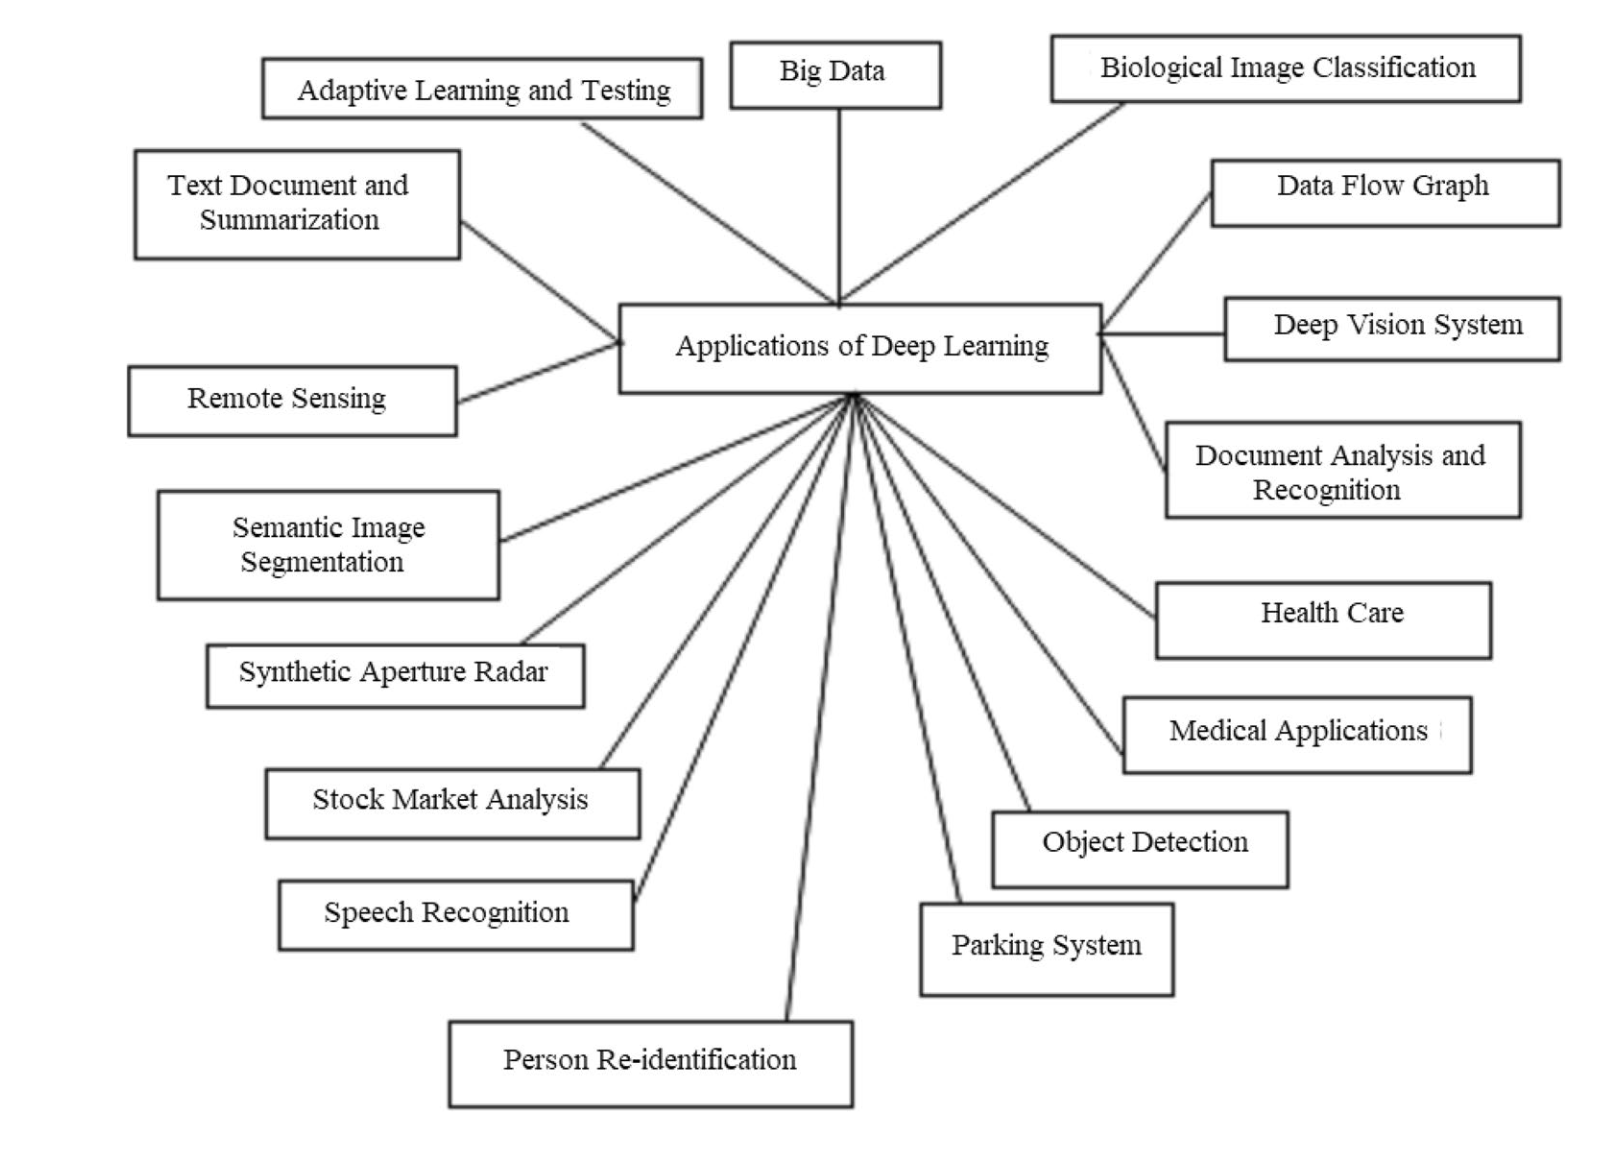
\includegraphics[scale=0.39]{img/applications_DL.png}
    \caption{Alcuni dei campi di applicazione del Deep Learning \cite{dlsurvey2}.}
    \label{fig:appl_dl}
\end{figure}
Un altro campo in cui il DL ha avuto molto successo è stato quello dell'analisi d'immagini. In particolare, per alcuni task come la classificazione e la segmentazione, le reti neurali hanno apportato netti miglioramenti. Infatti, a partire dal 2012, quando l'AlexNet \cite{alexnet} (Figura \ref{fig:alexnet}) vinse la ImageNet challenge battendo gli altri concorrenti con una un rateo di errore di circa il 16\%, contro il 26\% del vincitore dell'anno precedente, le reti neurali hanno sempre dominato le challenge riguardanti task di Computer Vision. 
Un'altra peculiarità del DL, che lo distingue dal ML e che lo rende così efficiente in campi come la Computer Vision, è che la fase di \textit{feature extraction} del ML, in cui vengono manualmente estratte le feature dal dato, è implicita nell'apprendimento della rete neurale (Figura \ref{fig:ML_vs_DL}). Questa caratteristica risulta fondamentale in quanto spesso questa fase risulta molto complessa, sia per la difficoltà dell'estrazione stessa, soprattutto per dati di tipo immagine, sia perché spesso per conoscere quali siano le feature da estrarre, è necessaria una conoscenza specifica del campo di applicazione. Nelle reti neurali invece, è proprio attraverso il meccanismo di apprendimento che la rete capisce quali sono le feature importanti e che determinano la natura del dato.

\begin{figure}[h!]
  \hspace*{0.2in}
  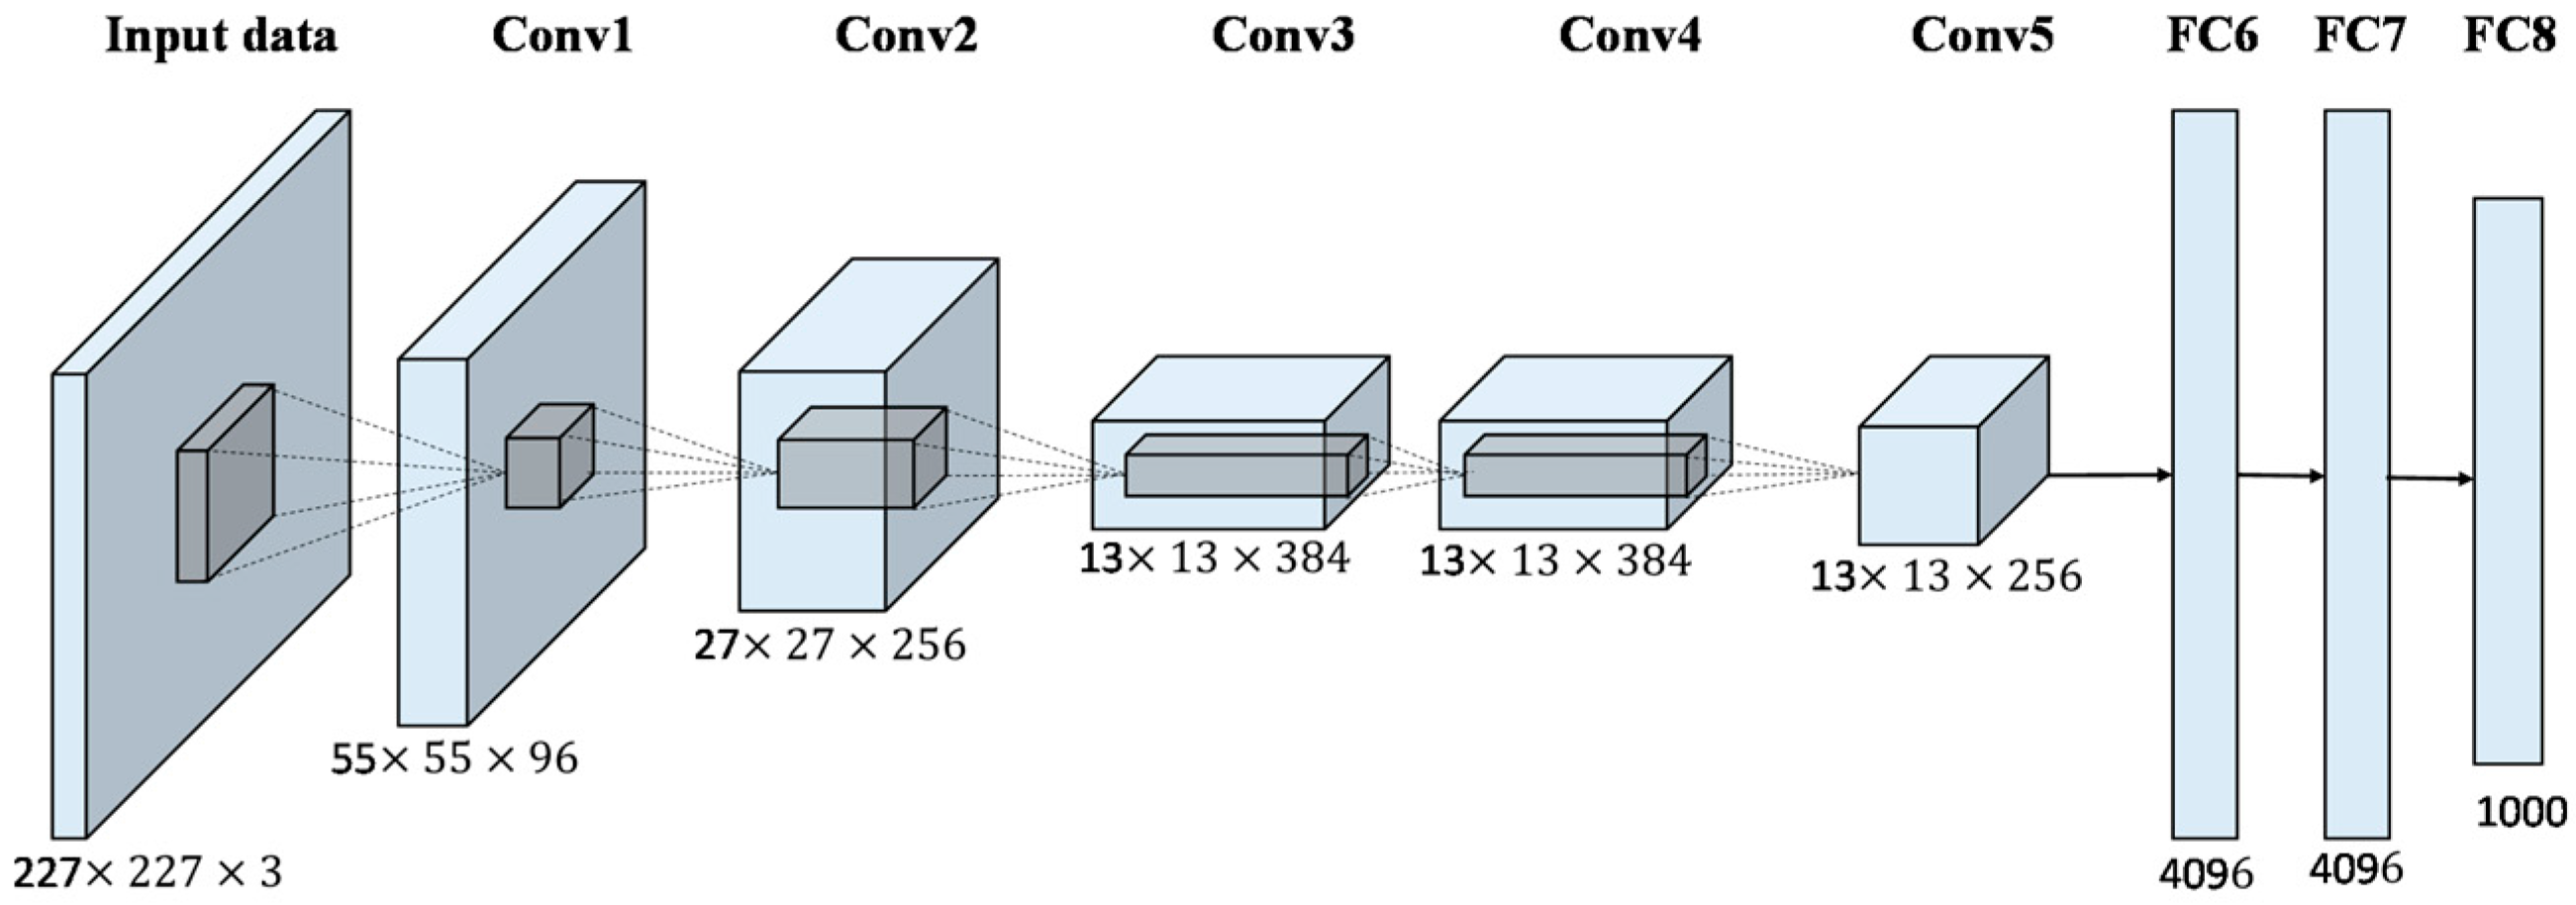
\includegraphics[scale=0.14]{img/alexnet2.png}
  \caption{Architettura della rete AlexNet.}
  \label{fig:alexnet}
\end{figure}

Oltre ai vantaggi, le reti neurali presentano anche diversi svantaggi. Uno di questi è che per alcuni aspetti le reti neurali sono dei modelli black-box. In particolare, il loro funzionamento è molto complesso e spesso, a differenza degli algoritmi di ML, il loro comportamento e i loro output diventano difficili da comprendere e di conseguenza da spiegare. Infatti negli ultimi anni, un campo dell'IA in forte crescita è l'Explainable AI \cite{expai}, che si occupa di algoritmi che forniscono trasparenza e interpretabilità a metodologie come le reti neurali.
\\ \\
\begin{figure}[h!]
    \centering
    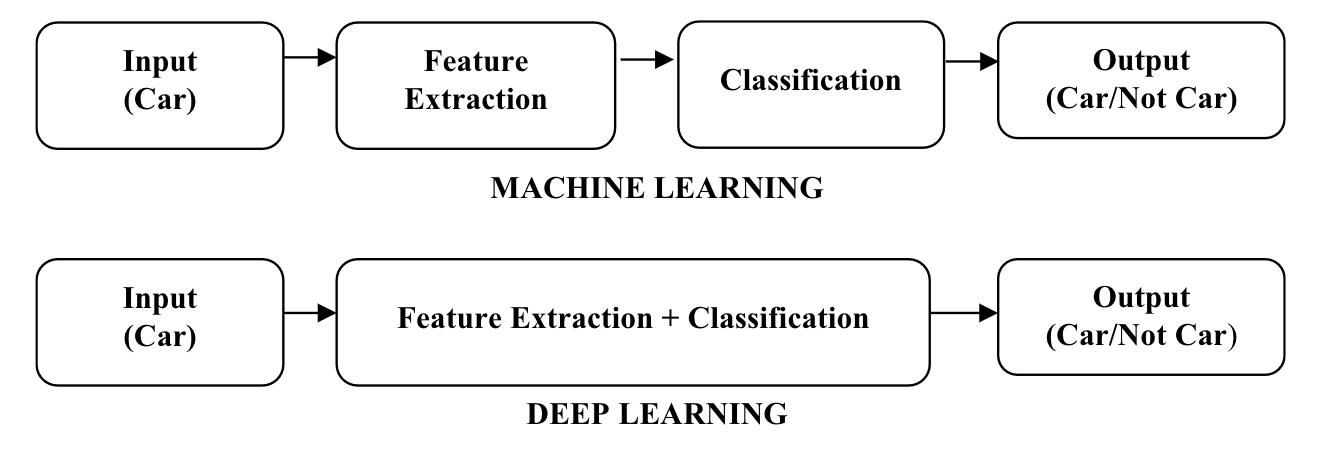
\includegraphics[scale=0.5]{img/ML_vs_DL.png}
    \caption{Differenza tra Machine Learning e Deep Learning \cite{dlsurvey2}.}
    \label{fig:ML_vs_DL}
\end{figure}




\section{Percettrone}
Il percettrone è un modello matematico ispirato al modello del neurone biologico \cite{rosenblatt1958perceptron} e costituisce il componente di calcolo di base delle reti neurali. Mentre il neurone biologico è costituito da quattro principali componenti (soma, dendriti, assone e sinapsi), il percettrone è composto da due parti (Figura \ref{fig:perceptron}): nella prima parte, viene calcolato il prodotto scalare tra il vettore d’input $X = (x_{1}, x_{2}, ..., x_{n})$ e i parametri del percettrone $W = (w_{1}, w_{2}, ..., w_{n})$ , mentre nella seconda parte il risultato del prodotto scalare viene dato in input alla funzione di attivazione $g$, che ci restituisce uno scalare. Di seguito la formula dell'output del percettrone:
\begin{equation}
    y = g( \sum_{j=1}^{n}{x_{j}w_{j}} ).
\end{equation}


La funzione di attivazione è una parte critica del percettrone, in quanto fornisce alla rete la non linearità, proprietà fondamentale per approssimare funzioni non lineari complesse. In particolare, senza funzioni di attivazione, per quanto complesse e profonde  possano essere le reti neurali, non rappresenterebbero altro che una funzione lineare dell’input e diventerebbero un semplice regressore lineare. Più avanti vedremo nei dettagli quali sono le funzioni di attivazione più utilizzate nelle moderne reti neurali.\\ \\

\begin{figure}[h!]
  \hspace*{0.3in}
  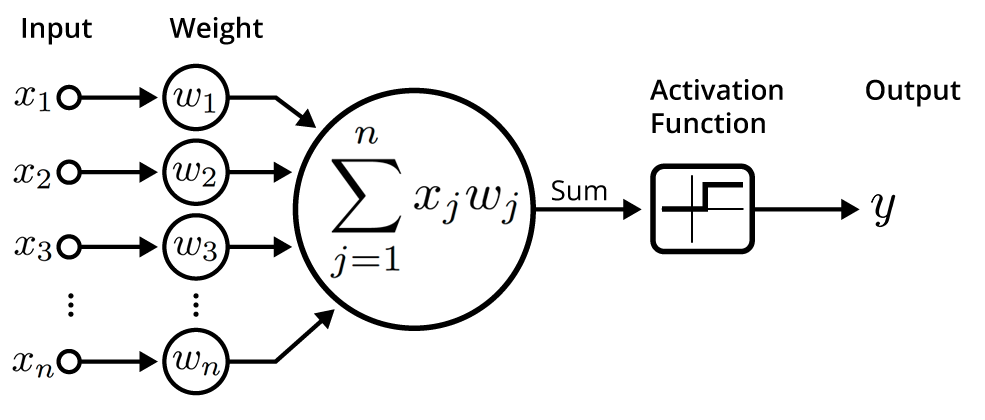
\includegraphics[scale=0.35]{img/neurone.png}
  \caption{Illustrazione della struttura di un percettrone.}
  \label{fig:perceptron}
\end{figure}














\section{Percettrone Multistrato}
Una delle tipologie più semplici di reti neurali è il Percettrone Multistrato, in inglese Multi-Layer Perceptron (MLP). L’MLP non è altro che un’insieme di percettroni collegati tra di loro e organizzati in strati (Figura \ref{fig:MLP}), dove gli output dei percettroni di uno strato sono l’input dei percettroni dello strato successivo. Gli strati, minimo tre, sono suddivisi in strato d’input, strato d’output e strati nascosti. Lo strato d’input è quello che riceve per primo il dato da elaborare, lo strato di output è quello che invece restituisce  l‘output finale della rete e  gli strati nascosti sono tutti gli altri che si trovano nel mezzo.\\

\begin{figure}[h!]
  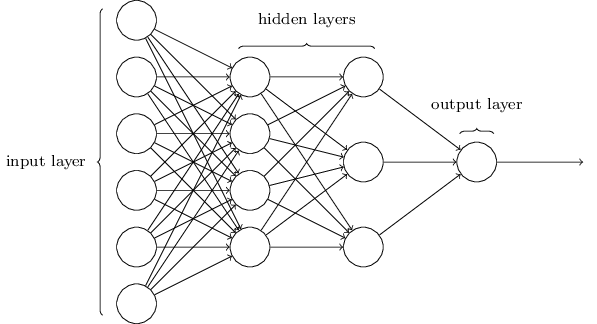
\includegraphics[scale=0.6]{img/MLP.png}
  \caption{Generica architettura di un Percettrone Multistrato.}
  \label{fig:MLP}
\end{figure}

Come detto precedentemente, grazie all’utilizzo delle funzioni di attivazione, l’output finale della rete risulta una funzione complessa e fortemente non lineare dell’input, complessità e non linearità che aumentano con l’aumentare delle dimensioni della rete. Questa proprietà risulta fondamentale e peculiare delle reti neurali, che si distinguono dagli altri modelli di ML proprio per la capacità di rappresentare funzioni molto complesse. Infatti, le reti neurali hanno preso il sopravvento soprattutto in quei task dove le funzioni o i pattern da apprendere sono molto complessi,  come nel campo dell’analisi di immagini.












\section{Funzioni di attivazione}
Come detto precedentemente, le funzioni di attivazione rappresentano un concetto cardine delle reti neurali. In particolare, la scelta delle funzioni di attivazione è una scelta fondamentale e può avere un grande impatto sulle performance del modello. All’interno di una rete, spesso vi sono diverse tipologie di funzioni di attivazione e nella maggior parte dei casi, se ne usano diverse tipologie per le diverse parti della rete. Tipicamente, gli strati nascosti utilizzano la stessa tipologia, mentre la scelta di quella dello strato di output dipende soprattutto dal task e dal tipo di output che bisogna fornire.
Di seguito, le funzioni di attivazione più utilizzate e presenti in letteratura.

\subsection{Funzione sigmoidea}
Una delle più note è la funzione sigmoidea (Figura \ref{fig:sigmoid}), anche detta sigmoid, una funzione matematica con la tipica curva ad S o curva sigmoid. In particolare, la sigmoid non fa altro che mappare l’input (un qualsiasi reale) su un range che va da 0 a 1: più l’input è grande e più sarà vicino a 1, mentre più sarà piccolo e più sarà vicino a 0. Di seguito la formula:
\\
\begin{equation}
\sigma(x) = \frac{1}{1+e^{-x}}.
\end{equation}
\\
La sigmoid viene spesso utilizzata nell’ultimo strato della rete neurale, soprattutto nei task di classificazione binaria, dove l’output finale della rete deve essere mappato nell’intervallo [0,1], in quanto rappresenta la probabilità che l’input appartenga a una delle due classi predeterminate.\\ \\

\begin{figure}[h!]
  \hspace*{0.9in}
  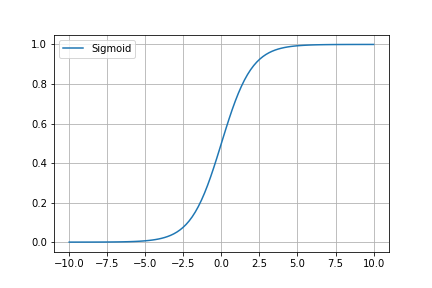
\includegraphics[scale=0.6]{img/sigmoid.png}
  \caption{Grafico della funzione sigmoidea.}
  \label{fig:sigmoid}
\end{figure}

\subsection{Tangente iperbolica}
La tangente iperbolica (Figura \ref{fig:tanh}), detta spesso “tanh”, è una funzione di attivazione molto simile alla sigmoid. La principale differenza è che mappa l’input nell’intervallo $[-1, +1]$ invece che in $[0, +1]$.\\ \\


\begin{figure}[h!]
  \hspace*{0.9in}
  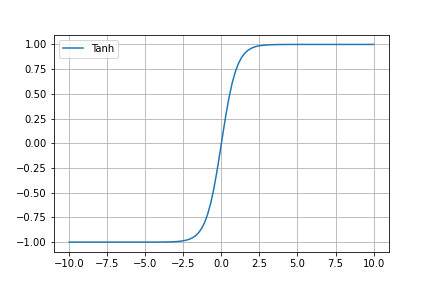
\includegraphics[scale=0.6]{img/tanh.png}
  \caption{Grafico della tangente iperbolica.}
  \label{fig:tanh}
\end{figure}










\subsection{Rectified Linear Activation Function}
La ReLU (Rectified Linear Unit) (Figura \ref{fig:relu}) è forse la funzione di attivazione più utilizzata. Il motivo sta nel fatto che risolve uno dei principali problemi delle funzioni di attivazione, ovvero la scomparsa del gradiente. Quest'ultima riguarda il fatto che nel meccanismo di retropropagazione (che affronteremo più avanti), soprattutto quando si hanno molti strati, i gradienti che vengono moltiplicati, se hanno valori piccoli, tendono ad andare verso lo 0 molto velocemente e questo porta ad avere cambiamenti, soprattutto nei primi strati della rete (gli ultimi nella retropropagazione), molto piccoli se non nulli. Di seguito la formula:
\\
\begin{equation}
  f(x) = x^{+} = max(0,x).
\end{equation}
\\
Inoltre la ReLU, vista la sua formula, risulta anche molto più semplice da calcolare rispetto alle altre e questa proprietà diventa critica soprattutto nelle reti neurali, dove spesso il costo computazionale diventa un ostacolo. Dall’altra parte, uno svantaggio della ReLU risiede nel fatto che per il valori negativi, la funzione ha una derivata nulla. Mentre questo può essere anche un punto di forza (per la sparsità della rete), rappresenta un problema quando molti dei valori in input alle funzioni di attivazione sono negativi perché molti dei neuroni vengono azzerati. Quando questo succede la rete tende a "morire" , ovvero tende a non aggiornare più i suoi parametri (da qui il nome del problema Dying ReLU).
Per risolvere questo problema, è stata introdotta una variante chiamata Leaky ReLU o ReLU Parametrica (Figura \ref{fig:leaky_relu}). In particolare, la variante, a differenza della versione originale, presenta nella parte negativa una piccola pendenza, che non è un parametro appreso durante l’addestramento, ma viene scelto in precedenza.\\ \\



\begin{figure}[h!]
  \hspace*{0.9in}
  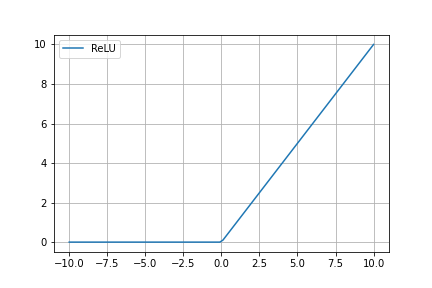
\includegraphics[scale=0.6]{img/relu.png}
  \caption{Grafico della ReLU.}
  \label{fig:relu}
\end{figure}


\begin{figure}[h!]
  \hspace*{0.9in}
  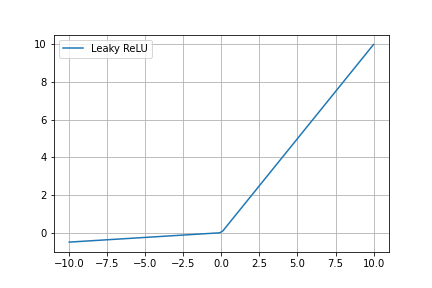
\includegraphics[scale=0.6]{img/leaky_relu.png}
  \caption{Grafico della Leaky ReLU.}
  \label{fig:leaky_relu}
\end{figure}






\subsection{Softmax}
Nei problemi di classificazione multiclasse, dove il numero di classi è maggiore di due, nello strato di output della rete non può essere usata la funzione sigmoid, che invece viene usata in ambito di classificazione binaria. Similarmente alla sigmoid, l'output della softmax può essere interpretato come le probabilità associate ad ogni classe, infatti tutti i valori sommati restituiscono 1. Quando il numero di classi è uguale a due, la softmax è equivalente alla sigmoid e volendo si può considerare la sigmoid un particolare caso della softmax o, in modo equivalente, la softmax una generalizzazione della sigmoid.
Di seguito la formula della softmax.
\\

\begin{equation}
softmax(x_{i}) = \frac{e^{x_{i}}}{\sum_{j}{e^{x_{j}}}}.
\end{equation}





\section{Apprendimento}
La fase di apprendimento è una fase in comune a tutti gli algoritmi di ML. In generale, in questa fase il modello che viene addestrato aggiorna i propri parametri cercando di migliorare le proprie performance, ovvero cercando di approssimare nel miglior modo possibile il pattern d'interesse.

\subsection{Paradigmi di apprendimento}
Nel campo del ML, esistono quattro principali paradigmi di apprendimento:

\begin{itemize}
    \item \textit{Supervisionato}: come detto in precedenza, l'approccio del ML si differenzia dall'approccio tradizionale nel fatto che chi sviluppa il modello non definisce le regole di funzionamento del mondo d'interesse, ma piuttosto si occupa di costruire un'architettura in grado di apprenderle dai dati. Detto ciò, risulta critico il ruolo dei dati. Infatti, soprattutto nel campo del DL dove i pattern del mondo d'interesse sono molto complessi, è fondamentale fornire al modello dati di quantità sufficiente, oltre che rappresentativi. In questo paradigma viene fornito al modello un insieme di dati, chiamato \textit{dataset}, composto da sole coppie di tipo X e Y, dove la X rappresenta l'input e la Y rappresenta il corretto output. Le coppie che compongono il dataset vengono utilizzate dal modello come esempio del funzionamento del pattern che sta cercando di approssimare.
    
    \item \textit{Non supervisionato}: in questo paradigma invece, nel dataset fornito c'è solo l'input senza il corretto output. Chiaramente, questo paradigma viene utilizzato solamente quando ottenere le corrispondenti label non è possibile oppure molto difficile. Un esempio di ciò è il campo delle immagini mediche, in cui solo degli specialisti possono produrre le label. Un altro esempio è quando la loro produzione risulta un processo molto lungo e tedioso, cosa che avviene spesso nell'ambito della segmentazione. Quando questo succede e il modello non ha esempi di input-output su cui basarsi, l'approccio più tipico è quello di cercare negli elementi del dataset delle similarità, in modo da poterli raggruppare in quelli che vengono chiamati \textit{cluster}.
    
    \item \textit{Semi Supervisionato}: questo paradigma è un punto d'incontro tra il paradigma supervisionato e quello non supervisionato. In particolare, in questo caso solo ad una parte del dataset è associata la corrispondente label.
    
    \item \textit{Per rinforzo}: qui il modello, detto anche \textit{agente}, apprende interagendo con l'ambiente esterno. In particolare, l'agente compie delle azioni e successivamente ne valuta i risultati, utilizzando un valore numerico di "ricompensa", che ha l'obiettivo di incoraggiare azioni correte e scoraggiare quelle scorrette.

\end{itemize}

\subsection{Funzioni di perdita}
Nella fase di apprendimento, un aspetto critico è come il modello valuta le proprie performance. In particolare, ad ogni iterazione dell'apprendimento il modello deve avere la capacità di valutare quanto il suo output sia distante da quello corretto. Di conseguenza, il modello per apprendere ha bisogno di una misura di questa distanza. Questo ruolo è ricoperto dalla funzione di perdita, che viene decisa dagli sviluppatori prima della fase di addestramento. La scelta della funzione di perdita è fondamentale e può avere un grande impatto sulle performance del modello. Una caratteristica fondamentale della funzione di perdita è la derivabilità. In particolare, è fondamentale in quanto la sua derivata viene utilizzata proprio per addestrare la rete (entremo nel dettaglio sul meccanismo di apprendimento più avanti). Di funzioni di perdita ne esistono molte tipologie che vengono scelte in base, soprattutto, al task:
\begin{itemize}
    \item nei problemi di regressione, ovvero dove l'output è un valore all'interno di un intervallo continuo, una delle funzioni di perdita più comuni è la \textit{MSE (Mean Squared Error)}, che calcola la media delle differenze al quadrato tra gli elementi del vettore delle predizioni \textit{pred} e gli elementi del vettore di output corretto \textit{y}.
    
    \begin{equation}
    MSE = \frac{1}{n}\sum_{y=1}^{n}(pred_{i} - y_{i})^{2}.
    \end{equation}

    \item nei problemi di classificazione binaria, una delle più utilizzate è la \textit{Binary Cross Entropy}.
    
    \begin{equation}
    BCE = -\frac{1}{n}\sum_{i=1}^{n}{(y_{i}\log(pred_{i}) + (1 - y_{i})\log(1 - pred_{i}))}.
    \end{equation}
    
    \item nei problemi di classificazione multiclasse, invece, viene spesso utilizzata la Cross Entropy
    \begin{equation}
    CE = -\frac{1}{n}\sum_{i=1}^{n}y_{i}\log(pred_{i}).
    \end{equation}
    
\end{itemize}

%\subsubsection{Focal Loss}
%Uno dei problemi che spesso emerge nell'affrontare un task di classificazione, rispetto a uno di regressione, è il bilanciamento delle classi del dataset. In particolare, questo problema sorge quando il numero di elementi del dataset appartenenti a una classe sono molti di più rispetto a quelli appartenenti ad un altra classe. Nel caso della segmentazione semantica, questo si trasforma nel avere classi a cui appartengono grandi porzioni delle immagini e classi a cui invece appartengono pochi pixel. Per esempio, nel dataset usato in questo lavoro, la classe \textit{prato} è molto presente e spesso ricopre una gran parte delle immagini, mentre la classe \textit{veicolo} è molto poco presente, sia a livello di numero di immagini in cui sono presenti veicoli sia a livello di numero di pixel che una veicolo ricopre. Il problema, è che le reti neurali che vengono addestrate su dataset che presentano questa caratteristica, spesso poi sono performanti nel riconoscere la classe più presente ma ottengono scarsi risultati nel riconoscere quella meno presente.
%Questo problema si può risolvere in diversi modi. Uno delle soluzioni più utilizzate è la funzione di perdita pesata, ovvero applicare ad ogni classe un peso che rappresenti l'importanza di riconoscere quella determinata classe. In particolare, alle classi più presenti vengono attribuiti pesi più bassi e a quelle meno presenti pesi più alti, in modo che, durante l'addestramento vengano più enfatizzati gli errori commesssi nel riconoscere classi meno presenti. Un esempio di questa tecnica utilizzata è la Cross Entropy Pesata, variante della funzione sopra menzionata.

%Durante questo lavoro, il problema dello sbilancimento delle classi del dataset, è stato uno dei principali problemi da affrontare e per risolverlo è stata utilizzata un particolare funzione di perdita chiamata \textit{Focal loss} \cite{focalloss}.








\subsection{Retropropagazione dell'errore}
Nelle reti neurali, così come in quasi tutti gli algoritmi di ML, la fase di apprendimento è una fase iterativa. Ad ogni iterazione, la rete, con i suoi parametri attuali, elabora uno o più elementi del dataset, confrontando poi l'output con la label corretta attraverso la funzione di perdita. A questo punto, la rete aggiorna i propri i parametri cercando di migliorare. Per capire come dovrebbe essere lo strato di output, abbiamo dei valori di riferimento, mentre per gli strati nascosti non abbiamo una diretta indicazione. L'aggiornamento dei parametri, generalizzata sia per lo strato di output che per quelli nascosti, è descritta dalla \textit{regola delta}:

\begin{equation}
\Delta w_{jk} = -\eta \delta _{j}o_{k}.
\end{equation}

Dove $\Delta w_{jk}$  è la variazione dei parametri tra il neurone $k$ e $j$, $\eta$ è il learning rate, $o_{k}$ è l'output dl neurone $k$, ovvero l'input del neurone $j$ e $\delta _{j}$ è l'errore dell'output del neurone $j$. La differenza tra strato d'output e strato nascosto sta nel valore di $\delta _{j}$, ovvero per lo strato d'output è il seguente

\begin{equation}
\delta _{j} = y_{j}(1-y_{j})(o_{j} - y_{j}).
\end{equation}

Dove $o_{j}$ è l'output del neurone $j$, mentre $y_{j}$ è l'output corretto.
Dall'altra parte, per gli strati nascosti è equivalente a 

\begin{equation}
\delta _{j} = y_{j}(1-y_{j})\sum_{k}\delta _{k}w_{kj}.    
\end{equation}

Dove invece $\sum_{k}\delta _{k}w_{jk}$ è la somma pesata degli errori di tutti i neuroni collegati a $j$. Infine, tutti i neuroni aggiornano i propri parametri utilizzando la seguente formula:

\begin{equation}
w_{jk} = w_{jk} + \Delta w_{kj}.
\end{equation}







\section{Regolarizzazione}
\label{regolarizzazione}
In generale, nel campo del Machine Learning, così come nel campo dell'ottimizzazione di funzioni, quello che si cerca di fare è minimizzare una funzione, o in altri termini, minimizzare un errore. La principale differenza tra i due campi è che, nel ML, oltre all'errore sul training set (\textit{training error}), viene anche preso in considerazione il \textit{test error}, anche detto "errore di generalizzazione". In particolare, alla fine della fase di addestramento, è importante che il modello costruito abbia delle buone performance non solo sui dati di addestramento (training set), ma anche e soprattutto su dati mai visti (test set) e questa abilità viene chiamata generalizzazione.
La capacità di un modello di saper generalizzare è molto importante e può dipendere da molti fattori. In particolare, oltre che dal giusto metodo e quantità di addestramento, dai giusti iperparametri e da molti altri fattori, la generalizzazione può soprattutto dipendere dalla scelta della complessità del modello. In generale, per quanto riguarda la complessità, il modello si può trovare in tre situazioni: nella prima il modello non ha approssimato bene il pattern interessato e la sua complessità è troppo bassa (\textit{underfitting}), nella seconda invece il modello è riuscito a cogliere il vero pattern e infine, nella terza situazione, il modello costruito ha alzato troppo la sua complessità, approssimando un pattern più complesso ma che include quello interessato (overfitting) (Figura \ref{fig:under-overfitting}). 

\begin{figure}[h!]
  \hspace*{-0.2in}
  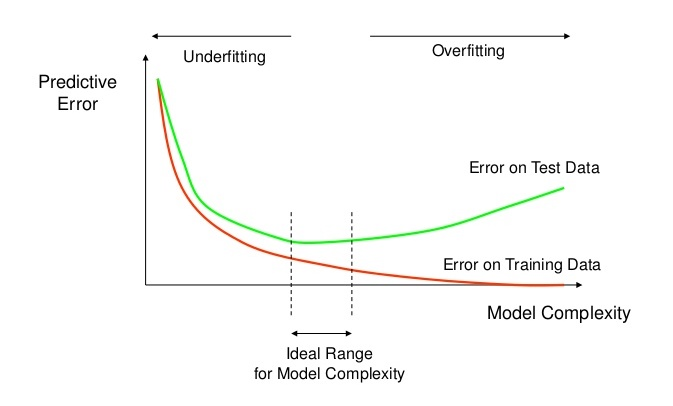
\includegraphics[scale=0.6]{img/over_underfitting.jpeg}
  \caption{Grafico degli errori sul training set e sul test set in funzione della complessità del modello e illustrazione dei due stati di underfitting e overfitting.}
  \label{fig:under-overfitting}
\end{figure}


Nel caso della prima situazione ci sono diverse soluzioni, ma in generale vanno riviste le scelte di design del modello e in ogni caso va aumentata la sua complessità. Nel caso dell'overfitting, invece, un metodo molto utilizzato è quello della regolarizzazione, il cui obiettivo è proprio quello di portare il modello dalla terza alla seconda situazione. In generale, possiamo definire la regolarizzazione come qualsiasi modifica che apportiamo al nostro modello o all'algoritmo di apprendimento, con l'obiettivo di ridurre il suo errore di generalizzazione ma non quello di addestramento.
Spesso nella pratica, soprattutto nei campi di applicazione del Deep Learning, anche con un un modello molto complesso, non è detto che si riesca ad includere il pattern interessato. In particolare nel mondo del DL, i modelli sono applicati a domini estremamente complessi e, di conseguenza, quasi sicuramente il vero pattern è al di fuori di quello del modello. Questo comporta che nella maggior parte dei casi, la scelta migliore è quella di grandi modelli con un'alta complessità, affiancati dalle giuste tecniche di regolarizzazione \cite{goodfellow2016deep}.
\\ \\
Di tecniche di regolarizzazione ne esistono svariate, ma uno dei metodi generali più utilizzati è quello di limitare la complessità del modello, anche detta capacità, aggiungendo alla funzione di perdita una componente di penalità $\Omega(W)$, trasformando la funzione di perdita, o anche detta funzione obiettivo, $J(W; X,y)$ in $\tilde{J}(W; X,y)$ dove:

\begin{equation}
    \tilde{J}(W; X,y) = J(W; X,y) + \alpha\Omega(W).
\end{equation}

Dove $\alpha\in[0, \infty] $ è un iperparametro che rappresenta il peso del contributo della penalità, $W$ sono i parametri del modello, $X$ rappresenta i dati di training e $y$ l'output corretto. In particolare, questa componente rappresenta l'intenzione di voler penalizzare la complessità del modello, di conseguenza, con la sua aggiunta durante la fase di apprendimento, l'algoritmo non cerca solo di minimizzare il training error, ma anche la complessità del modello. Nel dettaglio, esistono diversi metodi di questo genere e in ognuno $\Omega(W)$ prende una diversa forma. Due dei metodi più noti ed utilizzati di questa categoria sono la regolarizzazione L1 e la regolarizzazione L2. Un altro metodo di regolarizzazione molto usato nelle reti neurali è il \textit{dropout}. Il funzionamento di questa tecnica è molto semplice e intuitivo: durante l'addestramento, con una certa probabilità $p$, alcuni nodi della rete vengono disattivati, trasformando così a tutti gli effetti la rete in una meno complessa e riducendo la sua complessità (Figura \ref{fig:dropout}). Nel dettaglio, così come anche le altre tecniche di regolarizzazione menzionate prima, il dropout tende a tenere i parametri del modello  più bassi possibili e lo fa evitando di far prevalere un nodo sugli altri. In particolare, disattivando a turno randomicamente i vari nodi, costringe la rete a non sbilanciare i propri parametri verso un nodo, ottenendo dei parametri più bilanciati e di conseguenza più piccoli, mentre senza il dropout, il rischio è che durante l'addestramento la rete possa aumentare di molto i parametri di un nodo e azzerare quelli di altri.

\begin{figure}[h!]
  \hspace*{0.4in}
  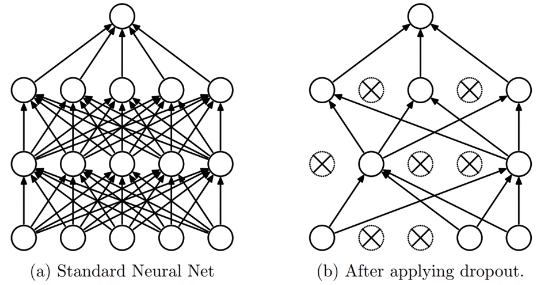
\includegraphics[scale=0.6]{img/dropout.png}
  \caption{Illustrazione della tecnica di dropout.}
  \label{fig:dropout}
\end{figure}




\subsection{Data augmentation}
\label{data_augmentation}
A parte le tecniche di regolarizzazione, il metodo sicuramente migliore per aumentare la capacità di generalizzazione di un modello è quello di fornigli più dati in input. Purtroppo però, come già detto, nella pratica i dati sono spesso molto difficili da reperire, soprattutto in alcuni campi di applicazione del DL. Spesso, per sopperire a questa difficoltà, si fa uso di una famiglia di tecniche di regolarizzazione chiamata \textit{data augmentation}. In generale, per data augmentation si intende una qualsiasi tecnica con cui si producono dati finti, partendo  da quelli veri. In particolare, partendo da uno o più elementi del dataset e applicando una trasformazione di qualche tipo, si può produrre un dato artificiale, ma comunque realistico. Questa tecnica viene spesso utilizzata nel campo della Computer Vision, dove le trasformazioni applicate ai dati sono ad esempio rotazioni, traslazioni, modifica del contrasto o della luminosità e molti altri (Figura \ref{fig:example-data_aug}). In questo campo, per alcuni task come la classificazione, la tecnica del data augmentation risulta spesso molto semplice, in quanto, dato che i classificatori devono risultare invarianti rispetto a molte trasformazioni dei dati \cite{goodfellow2016deep}, le trasformazioni fatte durante la data augmentation vanno applicate solamente alle immagini e non alle label, che invece devono rimanere uguali, cosa non vera, invece, nel campo della segmentazione semantica, dove andrebbero applicate in modo equo anche alle maschere.

\begin{figure}[h!]
  \hspace*{0.1in}
  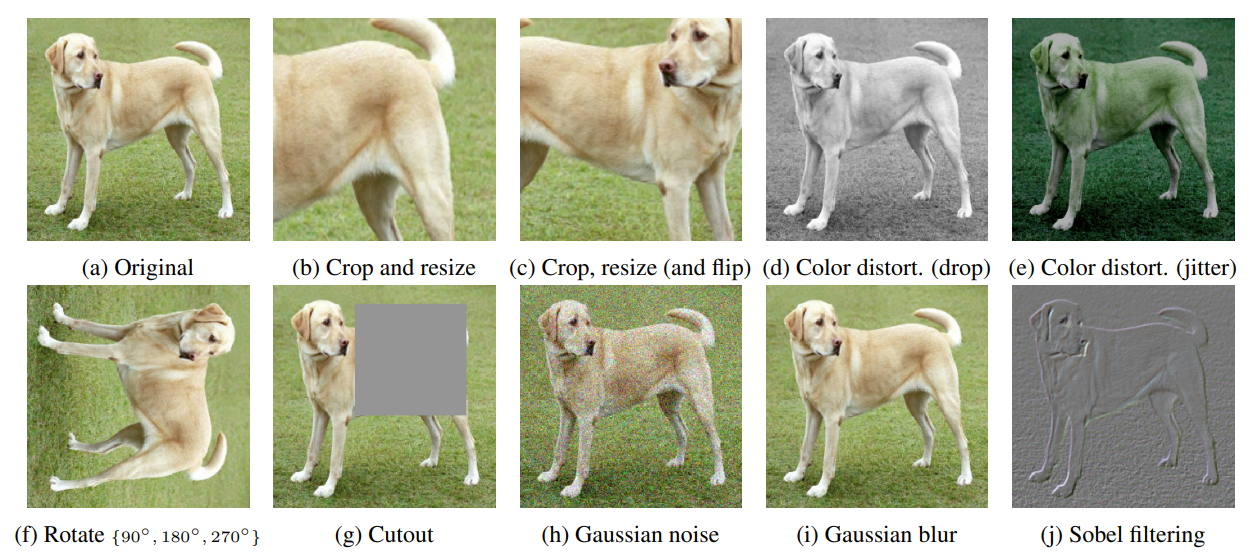
\includegraphics[scale=0.3]{img/example_data_aug.png}
  \caption{Alcuni esempi delle possibili trasformazioni per applicare data augmentation a un dataset d'immagini.}
  \label{fig:example-data_aug}
\end{figure}

Un'altra tipologia di data augmentation molto utilizzata è la \textit{noise injection}, ovvero la tecnica nella quale viene randomicamente applicato un certo rumore ai dati del dataset. Questa tecnica risulta spesso molto importante, poiché l'invarianza dei modelli rispetto al rumore nel dato in input è una caratteristica molto importante e desiderata, e la sua mancanza può portare a dei risultati negativi \cite{deep_trouble}, anche nell'ottica dell'Explainable AI. In particolare, spesso le immagini con l'aggiunta di un certo tipo di rumore risultano agli occhi umani identiche a quelle originali, di conseguenza il variare dell'output del modello da un'immagine all'altra può risultare un problema per l'interpretabilità del modello.
\\
Come precedentemente menzionato, la data augmentation risulta più semplice  per alcuni task, mentre per altri meno. Inoltre, recenti ricerche \cite{data_aug_effects} hanno dimostrato che questa tecnica può, da un lato portare a grandi miglioramenti nella capacità del modello di generalizzare, dall'altro penalizzare alcune classi. In particolare, i suoi effetti sono \textit{class-dependent}, ovvero dipendono dalla natura delle classi del dataset, di conseguenza l'utilizzo di queste tecniche può portare a miglioramenti in alcune classi, ma anche ad un calo delle performance in altre, soprattutto quando si applicano le stesse trasformazioni all'intero dataset.









\section{Reti Neurali convoluzionali}
Le reti convoluzionali \cite{convnets}, come il percettrone multistrato, presentano un layer d'input, uno di output e diversi layer nascosti. La differenza tra le reti classiche e quelle convoluzionali sta proprio nella presenza, tra quelli nascosti, degli strati convoluzionali (Figura \ref{fig:conv_net}). In particolare, le convoluzioni sono delle matrici la cui dimensione viene decisa in anticipo, che rappresentano dei filtri che vengono applicati sull'immagine scorrendo su di essa per estrarre determinati pattern. Uno dei principali vantaggi è che scorrendo sull'immagine, la convoluzione è in grado di riconoscere il pattern che ha appreso durante l'addestramento indipendentemente dalla posizione nell'immagine, a differenza delle normali reti neurali dove i neuroni, in particolare i primi, sono associati a precise porzioni dell'immagine. 

\begin{figure}[h!]
  \hspace*{0.1in}
  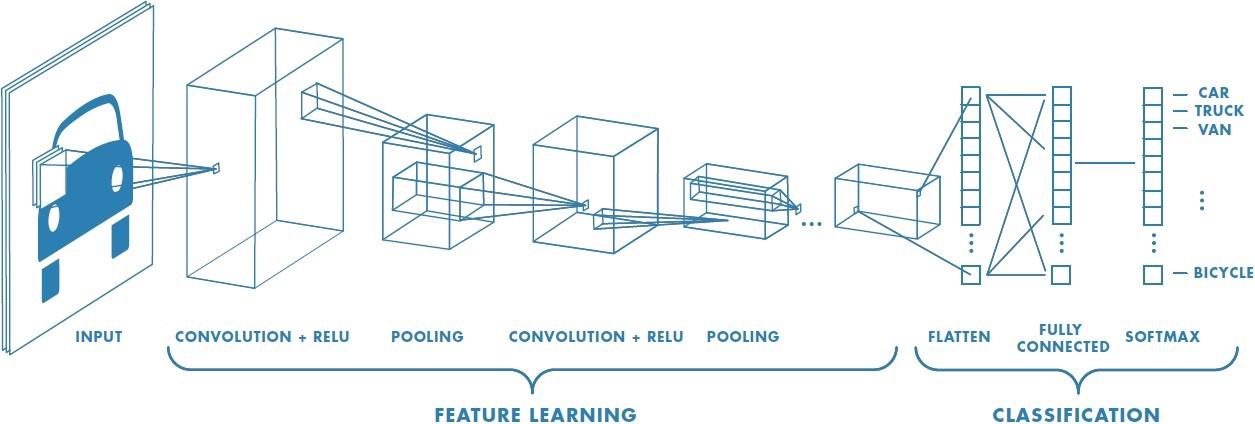
\includegraphics[scale=0.3]{img/conv_net.jpeg}
  \caption{Architettura di una generica rete convoluzionale.}
  \label{fig:conv_net}
\end{figure}

Le convoluzioni applicate alle immagini, anche chiamate \textit{kernel}, arrivano dal mondo della Computer Vision, dove vengono utilizzate per il processamento delle immagini. La differenza tra le convoluzioni tradizionali e quelle usate nelle reti neurali, sta nel fatto che mentre i valori di quelle tradizionali sono scelti in anticipo e pensati per applicare un determinato filtro, quelle nelle reti partono con dei valori inizializzati randomicamente, ed è proprio con l'addestramento che la rete impara quali sono i pattern da evidenziare. All'interno di una rete convoluzionale, solitamente, ci sono più strati convoluzionali e andando avanti nella rete, l'immagine in input diminuisce nelle prime due dimensioni (altezza e larghezza) e aumenta nella terza dimensione, ovvero quella del numero di feature, spesso chiamate canali. In particolare, ogni convoluzione applicata ad un'immagine produce una feature e più si va verso lo strato d'output, più le feature rappresentano pattern di più alto livello. Infatti, nei primi strati le feature rappresentano pattern più elementari, ad esempio forme geometriche come punti o linee. Negli strati più profondi invece, rappresentano strutture geometriche più complesse, oppure strutture con un significato semantico. La Figura \ref{fig:features} illustra in modo intuitivo il concetto appena spiegato.

\begin{figure}[h!]
  \hspace*{0.3in}
  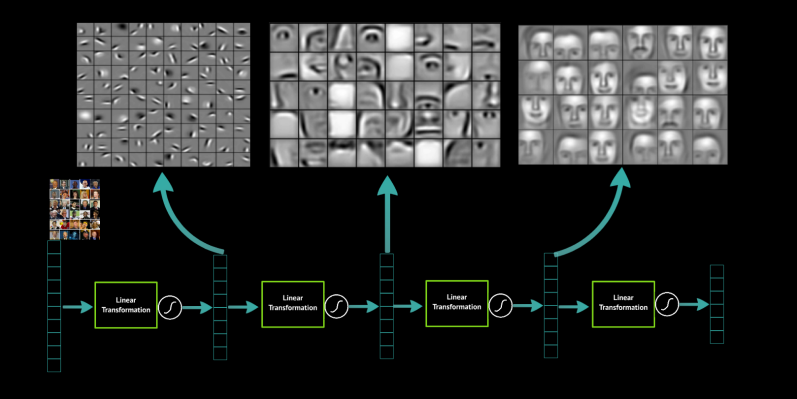
\includegraphics[scale=0.45]{img/features.png}
  \caption{Illustrazione del concetto di features di basso e alto livello.}
  \label{fig:features}
\end{figure}


Nella fase di costruzione della rete o successivamente nella fase di ottimizzazione degli iperparametri, riguardo le convoluzioni vanno stabiliti i valori di tre iperparametri:
\begin{itemize}
    \item \textit{dimensione del kernel}: la dimensione della matrice della convoluzione.
    
    \item \textit{stride}: indica il numero di pixel con cui la finestra si muove ad ogni operazione.
    
    \item \textit{padding}: denota il processo di aggiunta di zeri a ciasciun lato dell'input e questo iperparametro indica quanti aggiungerne. In particolare, il padding ha lo scopo di poter passare il kernel anche sui pixel più vicini ai bordi, e gli zero aggiunti servono proprio a riempire la parte del kernel che esce dall'input (Figura \ref{fig:padding}).
\end{itemize}

\begin{figure}[h!]
  \hspace*{1.7in}
  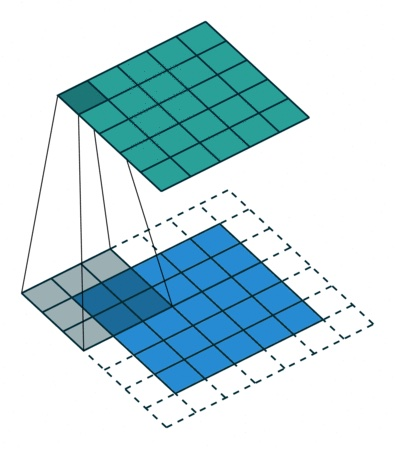
\includegraphics[scale=0.4]{img/padding2.jpg}
  \caption{Illustrazione del padding.}
  \label{fig:padding}
\end{figure}

Oltre agli strati convoluzionali, solitamente ci sono altre quattro tipologie di strati in una rete convoluzionale:
\begin{itemize}
    \item \textit{strato di pooling}: questo strato ha il ruolo di ridurre le prime due dimensioni del dato che attraversa la rete e anch'esso è un sorta di finestra che scorre sull'immagine, dando in output uno scalare. Ne esistono diverse tipologie, ma in generale, per una finestra dell'input restituisce un valore statistico di quest'ultima. Una delle tipologie più utilizzate è il \textit{max pool}, che restituisce il valore massimo all'interno della finestra; un altro molto usato è l'\textit{average pool}, che invece restituisce la media di tutti i valori nella finestra. A differenza della convoluzione, lo strato di pool non ha parametri apprendibili e il suo unico parametro è la dimensione della finestra, che più aumenta più riduce l'altezza e la larghezza del dato. L'importanza dello strato di pooling sta nel fatto che fornisce allo strato successivo l'invarianza rispetto a piccole traslazioni dell'input, ovvero modificando leggermente l'input dello strato di pooling, la maggior parte del suo output rimane invariato. Questa invarianza è fondamentale, soprattutto in alcuni task come la classificazione, in cui non è tanto importante dove sia la feature, ma piuttosto la sua presenza.
    
    \item \textit{strato di attivazione}: questa è una tipologia di strato in comune con tutte i tipi di rete neurale. Infatti, come già detto, questo strato ha il ruolo di fornire la non linearità alla rete, fondamentale per approssimare pattern complessi. Nel caso delle reti convoluzionali, la funzione di attivazione più comune è la ReLU e segue spesso gli strati di convoluzione.
    
    \item \textit{strato completamente connesso}: questa tipologia di strato, anche chiamato strato denso, è a tutti gli effetti strutturato come un percettrone multistrato e si trova sempre alla fine della rete. Questa parte della rete è la parte responsabile della classificazione, ovvero le feature ad alto livello prodotte dai primi strati vengono passate in input ai neuroni dello strato completamente connesso, così da produrre l'output finale.
    
    \item \textit{strato di attivazione finale}: questo strato rappresenta l'ultimo strato della rete ed ha il ruolo di traslare l'output nel range desiderato. Le due tipologie più utilzzate sono la \textit{sigmoid}, nel caso di classificazione binaria, e la softmax, nel caso di classificazione multiclasse.
\end{itemize}



\subsection{Reti neurali convoluzionali avanzate}

\subsubsection{VGG}
Il lavoro \cite{vgg}, che propose nel 2014 l'architettura chiamata VGG (Visual Geometry Group, ovvero il nome del gruppo di ricerca del lavoro) investigò il ruolo della profondità delle architetture nelle performance delle reti convoluzionali. Da questo studio ne risultò una delle architetture più note nel campo delle reti convoluzionali e della Computer Vision. Per quanto riguarda la struttura generale dell'architettura (Figura \ref{fig:vgg}), che però presenta diverse versioni a seconda della profondità, è composta da un primo strato, ovvero quello che prende in input l'immagine, che ha una dimensione fissa di 224x224, di conseguenza con questa versione della rete, tutte le immagini date in input devono avere quella dimensione e questo aspetto è dovuto al fatto che alla fine della rete sono presenti degli strati densi, anche detti \textit{fully connected} (FC), che non permettono alla rete di avere input di dimensioni diverse. Dopodichè, questo primo strato è seguito da uno stack di strati di convoluzioni 3x3, insieme, chiaramente, agli strati della funzione di attivazione (ReLU), con stride 1 e padding 1 (in modo da preservare la risoluzione spaziale dopo la convoluzione). In alcuni strati della rete sono presenti gli strati di pooling (max pooling), in particolare, in totale sono 5 e presentano una finestra 2x2 con stride 2. Infine, l'ultima parte della rete è composta da tre strati densi, di cui il primo e il secondo hanno una dimensione di 4096 canali, mentre l'ultimo ne ha 1000, poichè è stata costruita per essere testata su ImageNet che ha 1000 classi e un ultimo strato di Softmax.


\begin{figure}[h!]
  \hspace*{0.4in}
  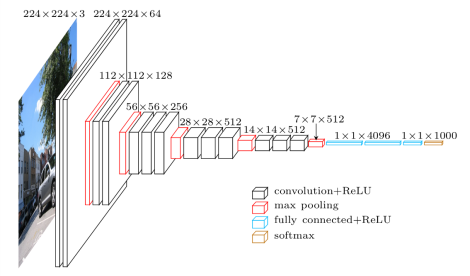
\includegraphics[scale=0.7]{img/vgg.png}
  \caption{Architettura generica della VGG.}
  \label{fig:vgg}
\end{figure}


Come detto precedentemente, l'architettura appena descritta assume diverse forme a seconda della profondità dello stack di convoluzioni. In particolare, le diverse versioni vanno da un minimo di 11 strati (8 strati di convoluzioni e 3 strati densi) fino ad un massimo di 19 (16 strati di convoluzioni e 3 strati densi), mentre l'ampiezza della rete (numero di canali) rimane coerente in tutte le versioni: parte da 64 fino ad arrivare negli ultimi strati di convoluzioni a 512.
La differenza principale tra la VGG e le architetture precedenti è soprattutto l'uso di convoluzioni piccole. In particolare, precedentemente la tendenza era quella di aumentare il campo ricettivo con convoluzioni sempre più grandi, come ad esempio nell'AlexNet \cite{alexnet}, che usa convoluzioni 11x11 con stride 4, oppure nell'archittetura proposta in \cite{visualizing_cnns} e nella OverFeat di \cite{overfeat}, che usano convoluzioni 7x7 con stride 2.
I vantaggi che gli autori di \cite{vgg} evidenziano riguardo l'uso di convoluzioni 3x3, sono principalmente dovuti al fatto che lo stesso campo ricettivo prodotto da una convoluzione 7x7 è riproducibile con uno stack di tre convoluzioni 3x3, con il vantaggio di incorporare tre strati di attivazione, che rende la funzione totale più discriminativa, e al fatto che in questo modo si riducono il numero di parametri della rete. In particolare, uno stack di tre convoluzioni ha $3(3^{2}C^{2})=27C^{2}$ parametri, dove $C$ è il numero di canali dell'input, mentre una convoluzione 7x7 ha $7^{2}C^{2}$ parametri.






\subsubsection{DenseNet}
Un'altra delle architetture più note è la DenseNet \cite{densenet}, un modello di rete convoluzionale ispirato al modello \textit{feed-forward}. In particolare, la peculiarità della DenseNet è che, a differenza delle classiche reti convoluzionali all'interno delle quali con $L$ strati si hanno $L$ collegamenti, ovvero uno tra ogni strato e il suo successivo, questa architettura  presenta $\frac{L(L+1)}{2}$ collegamenti, ovvero uno tra ogni strato e tutti gli strati successivi (Figura \ref{fig:densenet}).

\begin{figure}[h!]
  \hspace*{0.6in}
  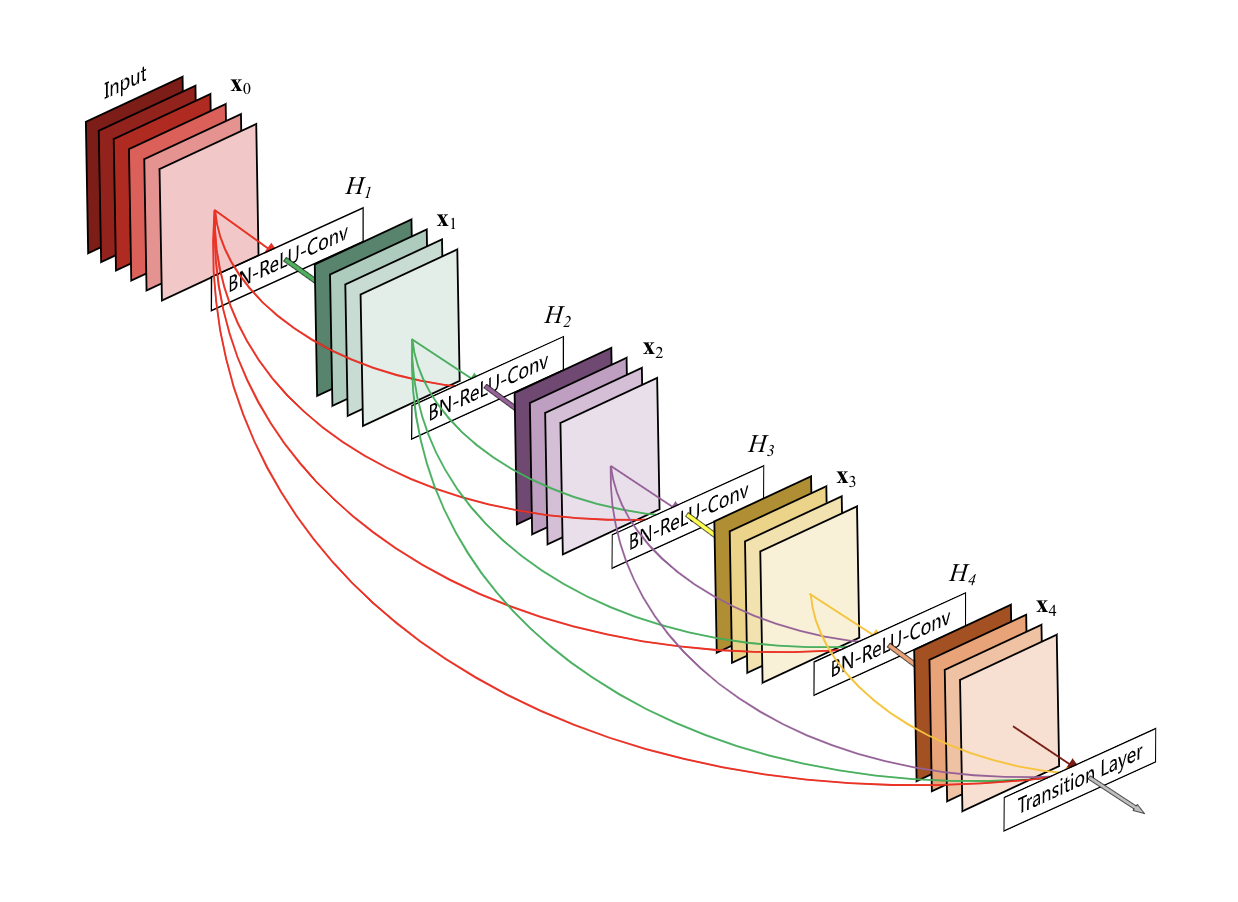
\includegraphics[scale=0.5]{img/densenet.png}
  \caption{Struttura di un blocco della DenseNet: ogni strato prende in input gli output di tutti gli strati precedenti \cite{densenet}.}
  \label{fig:densenet}
\end{figure}


I vantaggi evidenziati dagli autori di \cite{densenet} sono soprattutto riguardo uno dei maggiori problemi presenti nel campo delle reti neurali, ovvero la scomparsa del gradiente (\textit{vanishing gradients} in inglese). Come già menzionato, questo problema riguarda il fatto che nel meccanismo di retropropagazione dell'errore, quando si ha una rete molto profonda, si rischia che l'informazione sul gradiente, che viaggia dagli ultimi strati della rete fino ai primi, svanisca passando attraverso gli strati e non arrivi ai primi. In realtà, lo stesso problema può essere visto da un'altra prospettiva, ovvero nelle reti molto profonde non sono solo le informazioni sul gradiente a rischiare di scomparire, ma anche le informazioni sull'input che viaggiano dai primi agli ultimi strati. Nel corso degli anni, fino alla pubblicazione della DenseNet, in altri lavori \cite{resnets, huang2016deep, srivastava2015training, larsson2016fractalnet} questo problema è stato affrontato con diverse tecniche, che però hanno tutte avuto una cosa in comune, ovvero l'utilizzo di brevi connessioni per connettere strati vicini. Il lavoro fatto dagli autori, infatti, ha cercato di distillare e generalizzare questi approcci proposti precedentemente, creando un semplice schema di connessioni con l'obiettivo di massimizzare il flusso di informazioni tra gli strati della rete. Inoltre, a differenza di \cite{resnets}, la DenseNet, per minimizzare la perdita delle informazioni che giungono da strati precedenti, non utilizza la somma come operazione di fusione di diversi input, bensì la concatenazione.







\subsubsection{Modulo Inception e GoogLeNet}
Il lavoro \cite{inception}, seguendo la tendenza di quegli anni di aumentare sempre di più la complessità delle reti convoluzionali per aumentare le perfomance, ha avuto l'obiettivo di trovare un metodo per aumentare la complessità delle reti, senza però aumentare il suo costo computazionale. In particolare, l'idea dietro il loro lavoro è stata quella di creare un modulo, chiamato modulo "Inception", all'interno del quale venissero utilizzate contemporaneamente tutte le tipologie di componenti (convoluzioni con diverse dimensioni, pooling, ...), che solitamente venivano alternate strato per strato. L'intuizione di questo meccanismo è che la scelta dell'operazione da utilizzare per ogni strato non è più di chi costruisce il modello, ma del modello stesso, che ad ogni strato non è più limitato all'informazione della singola operazione fatta in quello strato, ma ha a disposizione le informazioni risultato di diverse operazioni fatte sullo stesso input. In particolare, la scelta degli autori su quali operazioni fare in parallelo nel modulo Inception è ricaduta su: convoluzione 1x1, convoluzione 3x3, convoluzione 5x5 e infine max pooling. Questa scelta è frutto di esperimenti fatti su diverse combinazioni, che come risultato hanno giudicato questa come la migliore. In realtà però, nei successivi sono state  proposte diverse varianti e nuove versioni del modulo Inception, che hanno utilizzato diverse combinazioni \cite{inceptionv2, inceptionv3, inceptionv4, xception}. Entrando nel dettaglio del suo funzionamento, il modulo Inception si basa sul dare lo stesso input parallelamente alle quattro diverse operazioni, i cui risultati vengono poi concatenati e passati al prossimo strato (Figura \ref{fig:inception_module_naive}). Per concatenare i quattro diversi output, chiaramente le loro prime due dimensioni (altezza e larghezza) devono coincidere, per far questo le tre operazioni di convoluzioni hanno dei parametri di stride e padding mirati. Per quanto riguarda il maxpooling, invece, che a differenza della convoluzione riduce per forza altezza e larghezza dell'input, è necessaria una certa quantità di padding per rendere il suo output coerente con gli altri.

\begin{figure}[h!]
  \hspace*{0.5in}
  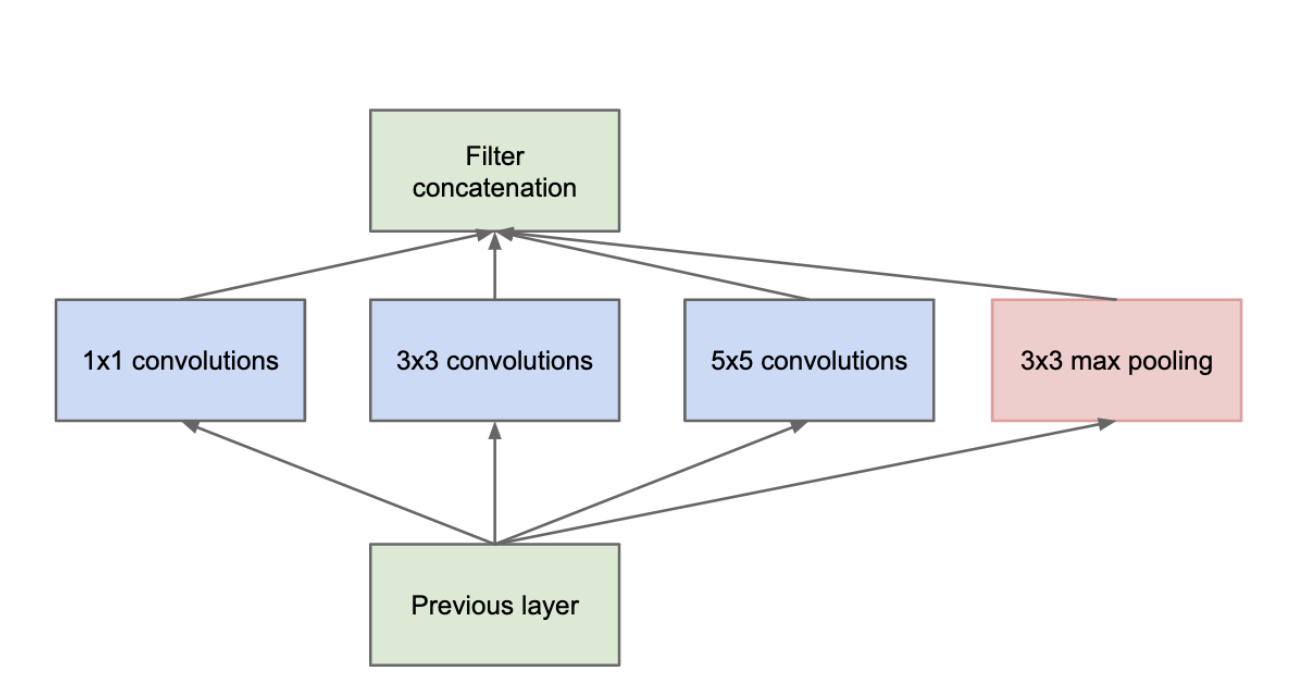
\includegraphics[scale=0.49]{img/inception-module_naive.png}
  \caption{Illustrazione del modulo Inception \cite{inception}, la versione senza riduzione delle dimensioni con costo computazionale molto alto.}
  \label{fig:inception_module_naive}
\end{figure}

Il problema di questa versione del modulo è che, aumentando di molto l'ampiezza degli strati della rete senza nessun tipo di accorgimento particolare,  anche il suo costo computazionale è aumentato. Per far fronte a questo aumento, gli autori hanno proposto un approccio che si basa sull'utilizzo di convoluzioni 1x1 per ridurre le dimensioni dell'input. In particolare, per le operazioni computazionalemente più costose, ovvero la convoluzione 3x3 e la convoluzione 5x5, aggiungono prima  una convoluzione 1x1, chiamata in questo caso \textit{bottleneck}, che ha lo scopo di portare l'input ad una dimensione per cui  applicare le convoluzioni ha un costo computazionale meno elevato. Inoltre, per quanto riguarda il maxpooling, la convoluzione 1x1 viene aggiunta dopo, dato che in questo caso non è tanto il costo computazionale dell'operazione a creare problemi, ma piuttosto la dimensione del suo output (che ha lo stesso numero di canali dell'input), il max pooling è seguito da una convoluzione 1x1, per far in modo di ridurre il numero di canali del suo output (Figura \ref{fig:inception_module}).

\begin{figure}[h!]
  \hspace*{0.6in}
  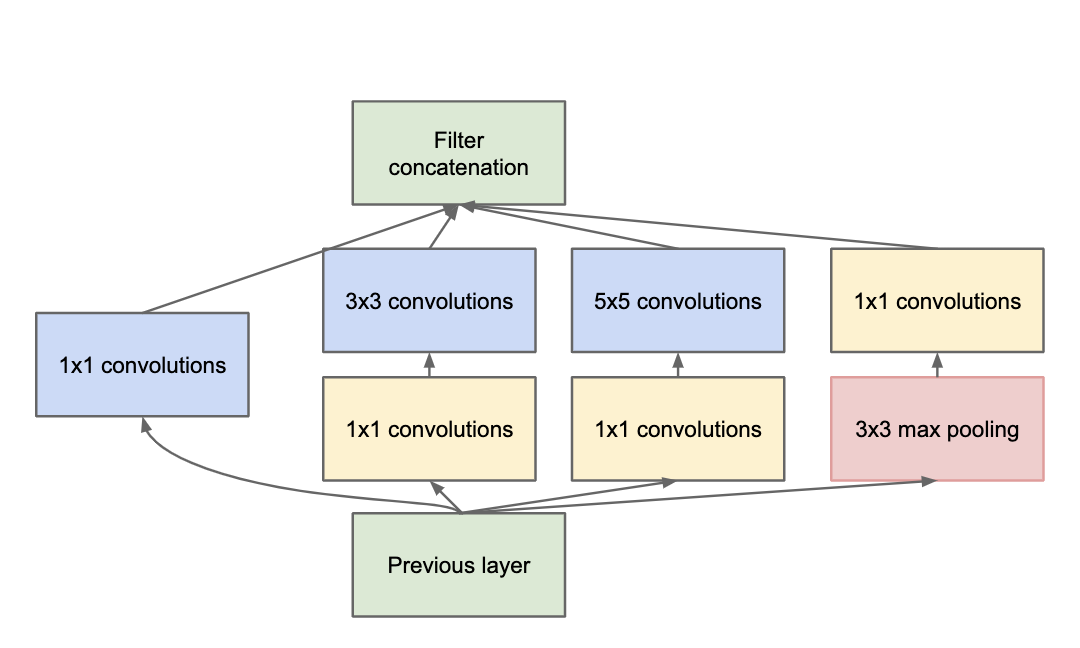
\includegraphics[scale=0.55]{img/inception.png}
  \caption{Illustrazione del modulo Inception \cite{inception}, la versione con la riduzione delle dimensioni attraverso strati di convoluzioni 1x1.}
  \label{fig:inception_module}
\end{figure}

Oltre alla concezione del modulo Inception, gli autori di \cite{inception} hanno anche proposto un'intera architettura basata proprio su questo tipo di modulo, la "GoogLeNet", il cui nome rende omaggio alla LeNet \cite{lenet}, una delle prime reti neurali convoluzionali sviluppate.
La GoogleNet (Figura \ref{fig:googlenet}), in particolare, è essenzialmente composta da uno stack di moduli Inception. Una sua peculiarità, al di là dell'uso del modulo Inception, è la presenza di due ulteriori strati intermedi di output. In particolare, la rete presenta in due dei moduli Inception dei rami addizionali di output, che terminano con uno strato di Softmax, trasformando l'output dei due strati intermedi in output effettivi della rete. A renderli due output effettivi della rete, è il fatto che la loss function totale, che la rete utilizza per addestrarsi, è calcolata con una somma pesata di tutti e tre gli output (questi due più quello finale), dando più peso a quello finale. Così facendo, la loss function  constringe la rete ad avere le feature map di quei due strati intermedi, già di una buona qualità per fare una predizione e l'idea dietro questo meccanismo è che si ottiene un effetto di regolarizzazione, spingendo la rete a non cadere nell'overfitting.


\begin{figure}[h!]
  \hspace*{1.3in}
  \includegraphics[scale=0.75]{img/googlenet.png}
  \caption{Architettura della GoogLeNet \cite{inception}.}
  \label{fig:googlenet}
\end{figure}




\chapter{Architettura e metodi del lavoro}
\label{chap_archi}
In questo capitolo vengono illustrati tutti i metodi utilizzati durante questo lavoro per affrontare la segmentazione semantica delle immagini del dataset FloodNet.
In particolare, l'intero lavoro si è basato sul cercare di risolvere le principali difficoltà trovate nell'affrontare questo dataset, che verranno approfondite nel Paragrafo \ref{difficolta_ds}.
Per quanto riguarda l'architettura utilizzata, l'idea base è stata quella di utilizzare un'architettura di Deep Learning, ovvero una rete neurale. La motivazione principale di questa scelta la si può trovare nel fatto che, come già evidenziato soprattutto nel paragrafo \ref{deep_learning}, le reti neurali riescono ad approssimare pattern molto più complessi rispetto ai metodi più tradizionali. Infatti, i lavori più attuali, che affrontano task simili a quello di questo lavoro \ref{stato_dell'arte}, utilizzano per la maggior parte metodi di Deep Learning. Nello specifico, la scelta dell'architettura DeepLabV3 \cite{deeplabv3}, si è basata invece sull'ovviare a due delle principali problematiche affrontate nel dataset (Paragrafo \ref{difficolta_ds}). 











\section{Difficoltà affrontate nel dataset}
\label{difficolta_ds}
Come spesso accade, le principali difficoltà affrontate durante questo lavoro sono state inerenti al dataset utilizzato. In particolare, questo aspetto è piuttosto comune, ovvero una grande porzione del tempo speso in questa tipologia di lavori spesso consiste nell'analizzare le caratteristiche del dataset per capirne le peculiarità, ma soprattutto le difficoltà.
Riguardo le specifiche difficoltà affrontate nel dataset FloodNet, di seguito se ne riportano le quattro principali:
\begin{itemize}
    \item le nove classi presenti all'interno del dataset sono fortemente sbilanciate. In particolare, alcune classi, come  "prato" e "albero", sono molto più presenti nel dataset rispetto ad altre classi, ovvero il numero di immagini che le contengono è molto più alto rispetto a quello delle altre.
    
    
    \item oltre allo sbilanciamento dal punto di vista delle occorrenze, le classi sono anche fortemente sbilanciate dal punto di vista della scala. In particolare, alcune classi, che sono  le stesse del problema menzionato sopra, sono rappresentate da regioni molto più grandi rispetto ad altre. Ad esempio, la classe "veicolo", così come la classe "piscina", è rappresentata da oggetti molto più piccoli rispetto a quelli della classe "prato" o "albero" e di conseguenza, aggiungendo il problema menzionato al punto precedente, il numero di pixel di queste classi all'interno del dataset risulta notevolmente  inferiore rispetto a quello di altre.

    
    \item alcune classi, più di altre, presentano una maggiore difficoltà intrinseca. In particolare, le due classi che sono risultate più difficoltose da apprendere sono state "strada allagata" e "edificio allagato". La motivazione, oltre ad essere presenti in misura minore all'interno del dataset, è soprattutto la loro natura semantica. Per quanto riguarda la classe "edificio allagato", la sua semantica deriva totalmente dal suo contesto e per nulla dalle sue caratteristiche locali. In particolare, se prendiamo solamente i pixel di un edificio, uno allagato è indistinguibile da uno non allagato, in quanto l'essere allagato o meno deriva dalla presenza di acqua di alluvione intorno all'edificio.
    Per quanto riguarda invece la classe "strada allagata", la sua semantica può derivare sia dal suo contesto, sia dalle sue caratteristiche locali, ma in alcuni casi grandi porzioni di una strada allagata possono essere indistinguibili da una non allagata. Nello specifico, una strada per essere considerata allagata non deve necessariamente presentare acqua in tutte le sue parti, ma è sufficiente una sola porzione allagata (Figura \ref{fig:strada_allagata}). 
    Inoltre, un'ulteriore difficoltà presente in entrambe le due classi sopra citate deriva dal fatto che la loro definizione risulta più vaga rispetto ad altre classi, prestandosi maggiormente a interpretazioni, caratteristiche che, nelle maschere del dataset, si presentano sotto forma di ambiguità.

    
    \begin{figure}[h!]
     \centering
     \begin{subfigure}[b]{0.45\textwidth}
         \centering
         \includegraphics[width=\textwidth]{img/7305.jpg}
         \caption{}
         \label{}
     \end{subfigure}
     \hfill
     \begin{subfigure}[b]{0.45\textwidth}
         \centering
         \includegraphics[width=\textwidth]{img/7305_lab.png}
         \caption{}
         \label{}
     \end{subfigure}
        \caption{Le due figure mostrano un esempio di come una strada allagata può presentare grandi porzioni senza acqua (nella parte in alto a destra), risultando indistinguibile da una strada allagata se non consideriamo il suo contesto.}
        \label{fig:strada_allagata}
    \end{figure}
    
    
    
    \item il dataset al suo interno presenta una grande quantità di rumore, ovvero in alcune maschere sono presenti degli errori. Inoltre, la maggior parte di questi errori sono proprio in immagini che presentano abbondanza di quelle classi menzionate nel punto precedente ("edificio allagato" e "strada allagata"). Di conseguenza, viste già le problematiche menzionate nei punti precedenti, la difficoltà nell'apprenderle aumenta ancora di più. Nello specifico, la maggior parte degli errori trovati nelle maschere del dataset può essere diviso in tre categorie:
    
    \begin{itemize}
        \item la prima tipologia di errore è rappresentata da maschere all'interno delle quali alcuni pixel sono classificati erroneamente. In particolare, i due casi più frequenti sono quelli in cui la classe "strada allagata" oppure la classe "prato" vengono invece classificati come "acqua" (Figura \ref{fig:problem_water}).
        
        \begin{figure}[h!]
         \centering
         \begin{subfigure}[b]{0.45\textwidth}
             \centering
             \includegraphics[width=\textwidth]{img/7245.jpg}
             \caption{}
             \label{}
         \end{subfigure}
         \hfill
         \begin{subfigure}[b]{0.45\textwidth}
             \centering
             \includegraphics[width=\textwidth]{img/7245_lab.png}
             \caption{}
             \label{fig:bottleneck}
         \end{subfigure}
            \caption{La figura mostra un esempio di errore presente nel dataset. In particolare, come si può notare i pixel che dovrebbero essere classificati come "prato" vengono invece classificati come "acqua".}
            \label{fig:problem_water}
        \end{figure}
        
        
        
        \item la seconda categoria invece, riguarda quei casi in cui alcune occorrenze di classi o parti di esse non vengono rappresentate nella maschera, ma i corrispettivi pixel vengono invece classificati come appartenti ad altre classi (Figura \ref{fig:problem_water}). I casi più frequenti riguardano le classi "strada" e "strada allagata".
        
        \begin{figure}[h!]
         \centering
         \begin{subfigure}[b]{0.45\textwidth}
             \centering
             \includegraphics[width=\textwidth]{img/7290.jpg}
             \caption{}
             \label{}
         \end{subfigure}
         \hfill
         \begin{subfigure}[b]{0.45\textwidth}
             \centering
             \includegraphics[width=\textwidth]{img/7290_lab.png}
             \caption{}
             \label{}
         \end{subfigure}
         \hfill
         \begin{subfigure}[b]{0.45\textwidth}
             \centering
             \includegraphics[width=\textwidth]{img/8445.jpg}
             \caption{}
             \label{}
         \end{subfigure}
         \hfill
         \begin{subfigure}[b]{0.45\textwidth}
             \centering
             \includegraphics[width=\textwidth]{img/8445_lab 2.png}
             \caption{}
             \label{}
         \end{subfigure}
            \caption{La figura mostra un esempio della seconda tipologia di errore presente nel dataset. In particolare, come si può notare, nella figura (b) una grossa porzione di un'occorrenza della classe "strada allagata" è mancante e i corrispettivi pixel vengono classificati come "acqua". Nella figura (d) invece un'occorrenza della classe "strada" non viene segnalata e i corrispettivi pixel vengono classificati come "prato".}
            \label{fig:problem_water}
        \end{figure}
        
        
        \item il terzo caso riguarda invece, la presenza di porzioni d'immagine fortemente incoerenti tra loro, oltre che con un certo grado di "confusione" tra le classi. La Figura \ref{fig:problem_confusion} ne illustra un esempio. 
        
        
        \begin{figure}[h!]
         \centering
         \begin{subfigure}[b]{0.45\textwidth}
             \centering
             \includegraphics[width=\textwidth]{img/7614.jpg}
             \caption{}
             \label{}
         \end{subfigure}
         \hfill
         \begin{subfigure}[b]{0.45\textwidth}
             \centering
             \includegraphics[width=\textwidth]{img/7614_lab 2.png}
             \caption{}
             \label{}
         \end{subfigure}
            \caption{La figura mostra un esempio della terza tipologia di errore presente nel dataset. In particolare, come si può notare, nella parte destra della maschera c'è un incoerenza rappresentata dal fatto che porzioni diverse della stessa strada vengono classificate come "strada non allagata" e "strada allagata", anche se vi è presenza di acqua. Inoltre, alcuni edifici circondati da strade allagate vengono classificati come "edificio non allagato". Infine, nella parte centrale dell'immagine viene segnalata un'occorrenza della classe "strada non allagata", quando in realtà nell'immagine non risulta.}
            \label{fig:problem_confusion}
        \end{figure}
        
    \end{itemize}
    
\end{itemize}










\section{Pulizia del dataset e Data Augmentation}
\label{data_aug_used}
Per far fronte a due delle quattro principali difficoltà menzionate nel paragrafo precedente, si sono messe in atto due fasi principali di pulizia del dataset (\textit{data cleaning}) e di data augmentation offline.
In particolare, queste due fasi sono risultate fondamentali per fornire un dataset composto da immagini elevate sia da un punto di vista qualitativo che quantitativo, fattore in generale  indispensabile per addestrare una rete neurale.
Partendo dalla pulizia del dataset, che è servita soprattutto ad ovviare al problema della presenza degli errori, questa fase è stata lunga e articolata, in quanto è stata effettuata una scansione manuale, confontando ogni immagine del dataset con la sua maschera corrispondente, al fine di individuare eventuali errori. Da questa scansione, si è riscontrato che in totale 182 immagini presentavano errori importanti, come quelli descritti nel paragrafo precedente. Di queste 182, ben 160 erano immagini contenenti entrambe le classi "allagate" (strada ed edificio). Confrontando quest'ultimo dato con il numero totale di immagini contenente queste due classi (all'incirca 200), si può notare come, oltre alle difficoltà intrinseche delle due classi, questa notevole presenza di errori le abbia fortemente svantaggiate. In seguito a questa fase di accertamento della consistenza del problema, si è proseguito con la fase di correzione. Durante questa fase, una parte degli errori è risultata corregibile attraverso diversi metodi, a seconda della natura dell'errore, altri invece, a causa della loro natura non hanno permesso la correzione in tempi non troppo lunghi e di conseguenza, per non rallentare troppo il lavoro, sono state scartate. In particolare, delle 182 totali, 45  non state corrette ma scartate. La Figura \ref{fig:esempio_correzioni} mostra un esempio di come una maschera contenente un errore sia stata corretta.
\\


\begin{figure}[h!]
    \centering
    \begin{subfigure}[b]{0.6\textwidth}
        \centering
        \includegraphics[width=\textwidth]{img/7252.jpg}
        \caption{}
        \label{}
    \end{subfigure}
    \hfill
    \begin{subfigure}[b]{0.45\textwidth}
        \centering
        \includegraphics[width=\textwidth]{img/7252_lab.png}
        \caption{}
        \label{}
    \end{subfigure}
    \hfill
    \begin{subfigure}[b]{0.45\textwidth}
        \centering
        \includegraphics[width=\textwidth]{img/7252_lab 2.png}
        \caption{}
        \label{}
    \end{subfigure}
    \caption{Le tre figure sono un esempio di correzione fatto sulle maschere del dataset FloodNet. La figura (a) è l'immagine a cui si riferiscono le due maschere (b) e (c). Come si può notare, nella (b) una porzione di prato è invece classificata come acqua (celeste), mentre la (c) è la versione corretta.}
    \label{fig:esempio_correzioni}
\end{figure}

Mentre la fase di pulizia ha cercato di ovviare soprattutto alla quarta problematica, la fase successiva di data augmentation offline ha invece cercato di risolvere soprattutto la problematica dello sbilanciamento verso alcune classi.

Come evidenziato dagli autori di \cite{data_aug_effects}, la data augmentation può creare degli effetti indesiderati, svantaggiando una classe rispetto ad altre. Per questo motivo, questa fase di data augmentation offline non è stata fatta su tutto il dataset, ma su un gruppo di immagini selezionate. In particolare, come già detto, lo scopo della selezione è stato di aumentare la presenza di quelle classi che riguardano la problematica dello sbilanciamento, specialmente le classi "strada allagata" e "edificio allagato", senza però sbilanciare ancora di più il dataset verso classi molto presenti, come la classe "prato". 
Per l'implementazione di questa data augmentation è stata utilizzata la nota libreria Albumentations \cite{albumentations} e il meccanismo generale è stato il seguente: ad ognuna delle 140 immagini selezionate è stata applicata per tre volte una combinazione randomica di quattro operazioni (non sempre tutte e quattro), producendo  per ogni immagine ulteriori tre (Figura \ref{fig:esempi_data_aug}). In particolare, le trasformazioni utilizzate sono: \textit{Rotate}, che consiste nella rotazione di una quantità randomica di gradi dell'immagine; \textit{VerticalFlip}, ovvero l'immagine viene ruotata su sé stessa sull'asse che la attraversa orizzontalmente; \textit{HorizontalFlip}, ovvero la stessa trasformazione ma sull'asse verticale; e infine \textit{RandomBrightnessContrast}, che consiste nell'alterare randomicamente la luminosità e il contrasto dell'immagine.

\begin{figure}[h!]
     \centering
     \begin{subfigure}[b]{0.45\textwidth}
         \centering
         \includegraphics[width=\textwidth]{img/7310.jpg}
         \caption{}
         \label{}
     \end{subfigure}
     \hfill
     \begin{subfigure}[b]{0.45\textwidth}
         \centering
         \includegraphics[width=\textwidth]{img/7310_lab.png}
         \caption{}
         \label{}
     \end{subfigure}
     \hfill
     \begin{subfigure}[b]{0.45\textwidth}
         \centering
         \includegraphics[width=\textwidth]{img/7310_0.jpg}
         \caption{}
         \label{}
     \end{subfigure}
     \hfill
     \begin{subfigure}[b]{0.45\textwidth}
         \centering
         \includegraphics[width=\textwidth]{img/7310_0_lab.png}
         \caption{}
         \label{}
     \end{subfigure}
     \hfill
     \begin{subfigure}[b]{0.45\textwidth}
         \centering
         \includegraphics[width=\textwidth]{img/7310_1.jpg}
         \caption{}
         \label{}
     \end{subfigure}
     \hfill
     \begin{subfigure}[b]{0.45\textwidth}
         \centering
         \includegraphics[width=\textwidth]{img/7310_1_lab.png}
         \caption{}
         \label{}
     \end{subfigure}
     \begin{subfigure}[b]{0.45\textwidth}
         \centering
         \includegraphics[width=\textwidth]{img/7310_2.jpg}
         \caption{}
         \label{}
     \end{subfigure}
     \hfill
     \begin{subfigure}[b]{0.45\textwidth}
         \centering
         \includegraphics[width=\textwidth]{img/7310_2_lab.png}
         \caption{}
         \label{}
     \end{subfigure}
     
        \caption{Le otto figure mostrano un esempio della data augmentation utilizzata offline prima dell'addestramento. Le figure (a) e (b) sono l'immagine e la maschera originali, mentre tutte le altre sono il risultato dell'applicazione di un sottoinsieme delle operazioni Rotate, HorizontalFip, VerticalFlip e RandomBrightnessContrast.}
        \label{fig:esempi_data_aug}
\end{figure}

 Oltre ad utilizzare la data augmentation offline, per aumentare il numero di immagini del dataset ed ovviare al problema dello sbilanciamento, è stata utilizzata una seconda fase di data augmentation online, ovvero durante l'addestramento. Lo scopo, in questo caso, non era aumentare il numero di immagini ma ottenere un effetto regolarizzante apportando ad ogni epoca dell'addestramento una diversa modifica ad ogni immagine. L'intuizione dietro questo metodo è che in questo modo, ad ogni epoca il modello vede una versione del dataset leggermente diversa e questo evita che andando avanti nell'addestramento il modello cada nel meccanismo di overfitting. In particolare, anche qui per l'implementazione è stata utilizzata la libreria Albumentations e il meccanismo generale è il seguente: durante un'epoca, ad ogni caricamento di un'immagine per la costruzione di una batch viene applicata un'operazione di \textit{VerticalFlip}, una di \textit{HorizontalFlip} e infine una di \textit{RandomBrightnessContrast}. La chiave di questo metodo è che, come nella data augmentation fatta offline, ad ogni trasformazione viene associata una probabilità, di conseguenza ad ogni epoca non vengono applicate tutte e tre le trasformazioni, ma solo un sottoinsieme randomico delle tre, creando nella pratica una versione diversa del dataset ad ogni epoca.














\section{DeepLabV3}
\label{paragr_deeplabv3}
Le principali difficoltà che gli autori di \cite{deeplabv1, deeplabv2, deeplabv3} hanno evidenziato riguardo l'applicazione delle DCNN al task generale della segmentazione semantica sono due: la prima si riferisce alla bassa risoluzione delle feature map prodotte dalle DCNN, mentre la seconda riguarda la presenza all'interno dell'immagine di oggetti a diversa scala. In particolare, soprattutto la seconda difficoltà presenta un forte parallelo con una delle principali problematiche affrontate in questo lavoro. Ed è proprio questa la motivazione per cui si è scelto di utilizzare questo modello. Riprendendo il discorso delle difficoltà delle DCNN nella segmentazione semantica, la prima difficoltà è soprattutto causata dalla combinazione e dall'alternarsi di strati di pooling e convoluzioni con stride. In particolare, questa è una caratteristica che rappresenta uno dei punti di forza delle DCNN in campi come la classificazione, dove ridurre la risoluzione delle feature map serve proprio ad apprendere rappresentazioni molto astratte del dato e ad acquisire l'invarianza rispetto a sue trasformazioni locali. Chiaramente, questo punto di forza si trasforma in una debolezza nel task della segmentazione, in cui la localizzazione è fondamentale. La seconda difficoltà invece, è causata dalla natura dei dati e riguarda sostanzialmente la presenza nell'immagine di oggetti di diverse dimensioni. Per risolvere la prima problematica, gli autori propongono un approccio basato sull'utilizzo di una particolare tipologia di convoluzione, ovvero la convoluzione dilatata (\textit{dilated convolution} o anche \textit{atrous convolution}). In particolare, gli autori propongono di rimuovere la fase di downsampling e utilizzare una convoluzione il cui kernel ha subito un upsample, inserendo dei vuoti al suo interno (Figura \ref{fig:dilated_conv}).
\\
\begin{figure}[h!]
    \centering
    \hspace*{0.1in}
    \includegraphics[scale=0.5]{img/dilated2.png}
    \caption{Illustrazione della differenza tra una convoluzione dilatata (a destra) e una normale convoluzione (a sinistra).}
    \label{fig:dilated_conv}
\end{figure}

Come detto in precedenza, la motivazione principale della scelta di questo modello specifico, consiste nel fatto che il lavoro degli autori mira proprio a risolvere il problema degli oggetti a diversa scala. In particolare, ispirandosi all'idea del SPP di \cite{pspnet}, propongono una simile struttura chiamata ASPP (Atrous Spatial Pyramid Pooling), che si basa sul concetto di utilizzare convoluzioni dilatate con diversa dilatazione in parallelo. Oltre a risolvere tale problematica, la DeepLabV3, essendo uno dei più noti modelli della categoria context-based \ref{context_based}, si presta a risolvere anche la problematica della difficoltà intrinseca delle due classi "edificio allagato" e "strada allagata".
Per quanto riguarda la specifica versione dell'architettura utilizzata in questo lavoro, per la prima parte della rete, chiamata \textit{backbone}, che ha il ruolo di produrre le feature map che verranno poi passate all'ASPP per produrre la maschera finale, viene utilizzata la ResNet101, ovvero una versione specifica dell'architettura basata su strati residui proposta in \cite{resnets}.









\subsection{Architettura totale}
Partendo dalla struttura generale dell'architettura, essa è composta da:
\begin{itemize}
    \item \textbf{backbone}: prima parte della rete responsabile della feature extraction. Produce a partire dall'immagine in input una feature map di 2048 canali. In particolare, viene utilizzata una versione modificata con convoluzioni dilatate della ResNet101.
    
    \item \textbf{DeepLabHead}: seconda parte della rete, responsabile della produzione della maschera finale. Composta dall'ASPP e da un blocco convoluzionale che produce un volume 9xHxW, dove 9 è il numero delle classi.
    
    \item \textbf{Interpolazione bilineare}: responsabile dell'ultima fase di upsampling, grazie alla quale l'output della DeepLabHead viene portata alle dimensioni originali dell'immagine.
\end{itemize}

\begin{figure}[h!]
    \centering
    \hspace*{-0in}
    \includegraphics[width=\textwidth]{img/architecture.png}
    \caption{Illustrazione dell'architettura totale utilizzata.}
    \label{fig:arch_totale}
\end{figure}












\subsection{Convoluzione Dilatata}
Come già detto, all'interno della DeepLabV3, la convoluzione dilatata viene utilizzata per far fronte al problema della ridotta risoluzione delle feature map. In particolare, il problema nasce quando, nella seconda parte della rete, le feature subiscono un upsample per tornare alla risoluzione originale e produrre l'output finale. Nello specifico, la qualità della maschera risultante è scarsa e non contiene informazioni spaziali molto dettagliate. Con l'utilizzo della convoluzione dilatata invece, accoppiata con l'interpolazione bilineare per la fase di upsample, la maschera prodotta contiene informazioni spaziali più dettagliate (Figura \ref{fig:atrous_conv}).

\begin{figure}[h!]
  \hspace*{0.2in}
  \includegraphics[scale=0.55]{img/dil_conv.png}
  \caption{Illustrazione della convoluzione dilatata in 2-D. Come si può notare, la maschera prodotta nella riga superiore (convoluzione classica) presenta informazioni più sparse e meno dettagliate rispetto alla maschera prodotta nella riga inferiore (convoluzione dilatata e interpolazione bilineare).}
  \label{fig:atrous_conv}
\end{figure}

Oltre al discorso inerente la risoluzione delle feature map, un altro vantaggio delle convoluzioni dilatate, molto utile nel contesto di questo lavoro, è la capacità di aumentare la dimensione di una convoluzione senza aumentare il numero di parametri e di conseguenza senza aumentare il costo computazionale dell'architettura, che diventa spesso un problema. In particolare, una delle funzioni principali delle convoluzioni è catturare il contesto di un pixel, ovvero la regione intorno al pixel, da cui dipende fortemente la sua semantica. Spesso però, il contesto di un pixel è più ampio di quello che la finestra della convoluzione, chiamata \textit{campo ricettivo}, può catturare e qui entra in gioco il vantaggio delle convoluzioni dilatate. In particolare, entrando nel dettaglio del loro funzionamento, esse presentano un parametro in più rispetto alla convoluzione tradizionale, chiamato dilatazione, che rappresenta la quantità di vuoti che vengono inseriti nel kernel. Più questo parametro aumenta, più la finestra si ingrandisce e più aumenta l'ampiezza del contesto catturato, non cambiando però il numero effettivo di parametri.
Inoltre, possiamo considerare le convoluzioni dilatate come una generalizzazione delle normali convoluzioni, in quanto le seconde sono un caso particolare delle prime, ovvero con la dilatazione impostata a 1 una convoluzione dilatata diventa una normale convoluzione. Generalizzando al caso di dati 1-D, l'output $y[i]$ di una convoluzione dilatata con parametri $w$ di lunghezza $k$, che prende in input $x[i]$ è definita come:

\begin{equation}
    y[i] = \sum_{k=1}^{K}{x[i+rk]w[k]}.
\end{equation}




\subsection{Reti Neurali Residue}
A partire dal 2012, per aumentare le performance delle reti neurali si sono costruiti modelli sempre più profondi, ed è nata la convinzione che aumentando sempre di più gli strati delle reti si possa ottenere una maggiore accuratezza. Questa convinzione, tuttavia, è stata sfatata. In particolare, si è dimostrato che, mentre in teoria reti più profonde possono approssimare pattern più complessi e di conseguenza ottenere performance migliori, nella pratica esiste una certa soglia al di sopra della quale l'accuratezza dei modelli si satura. Ad esempio, è stato dimostrato che la "profondità ottima" dei modelli testati sul noto dataset ImageNet è tra i 16 e i 30 strati, e che un modello con 18 strati performa meglio di uno con 34 (Figura \ref{fig:imagenet_plainet}). Un simile risultato lo possiamo notare anche con il dataset CIFAR-10, con cui testando un modello con 20 strati e uno con 56, il fenomeno è lo stesso (Figura \ref{fig:cifar10_plain}).



\begin{figure}[h!]
    \centering
    \hspace*{0in}
    \includegraphics[scale=0.5]{img/imagenet_plainnet.png}
    \caption{Addestramento su ImageNet di architetture senza strati residui (\textit{plain}). Le curve sottili denotano l'errore di training, mentre quelle in grassetto denotano l'errore di validation. Come si può notare, la rete con 34 strati ha il training error più alto di quella con 18 strati durante tutto l'addestramento \cite{resnets}.}
    \label{fig:imagenet_plainet}
\end{figure}


\begin{figure}[h!]
    \centering
    \hspace*{-0.27in}
    \includegraphics[scale=0.55]{img/cifar10_plainet.png}
    \caption{Addestramento su CIFAR-10 di architetture senza strati residui. Anche qui, durante tutto l'addestramento, la rete con più strati (56) ha sia il training error sia il test error più alto di quella con meno strati (20) \cite{resnets}.}
    \label{fig:cifar10_plain}
\end{figure}

La causa principale della saturazione dell'accuratteza risiede nella difficoltà di ottimizzare la rete a causa di problemi come la \textit{scomparsa del gradiente} e l'\textit{esplosione del gradiente}. Per alleviare questa difficoltà, è stato introdotto un tipo di strato chiamato strato residuo \cite{resnets}, ovvero uno strato all'interno del quale l'output non è $F(x)$ (dove $x$ è l'input dello strato) come nei normali strati di una rete,  bensì $F(x)+x$ (Figura \ref{fig:residual_block}). In particolare, l'input dello strato viene sommato all'output e questo meccanismo viene implementato con quelle che sono chiamate \textit{skip connections}. L'aggiunta della $x$ all'output dello strato risolve il problema della scomparsa del gradiente, poiché nel caso dell'azzeramento dei parametri dello strato, il suo output non sarebbe comunque azzerato, ma  sarebbe uguale all'input. Questo aspetto, oltre a risolvere la scomparsa del gradiente, rappresenta un secondo vantaggio degli strati residui, ovvero l'aggiunta di uno strato residuo non può causare particolari peggioramenti della rete, sia in termini di ottimizzazione che di performance. In particolare, l'aggiunta di uno strato residuo garantisce, oltre ai possibili miglioramenti discussi precedentemente, di non aggiungere particolari difficoltà all'ottimizzazione e di non peggiorare le performance della rete. Questa garanzia è data dal fatto che, nel caso in cui l'aggiunta non migliorasse le performance, comunque non ne complicherebbe più di tanto l'ottimizzazione, poichè con l'aggiunta della $x$, alla rete basta azzerare i parametri dello strato per approssimare la funzione identità. In particolare, la funzione identità prende in input $x$ e restituisce $x$, non cambiando di conseguenza l'output dello strato precedente. 


%la rete può facilmente apprendere i parametri dello strato per approssimare la funzione identità, che prende in input $x$ e restituisce $x$, non cambiando quindi l'output della versione della rete senza quello strato.


%comunque non ne complicherebbe più di tanto l'ottimizzazione, in quanto grazie all'aggiunta della $x$ la rete può facilmente apprendere i parametri dello strato per approssimare la funzione identità, che prende in input $x$ e restituisce $x$, non cambiando quindi l'output della versione della rete senza quello strato. In particolare, per approssimare la funzione identità, gli basta azzerare i parametri dello strato, ottenendo $F(x)=0$ e quindi l'output dello strato $F(x)+x=x$.

\begin{figure}[h!]
    \centering
    \hspace*{-0.1in}
    \includegraphics[scale=0.4]{img/residual_blocks.png}
    \caption{Illustrazione della differenza tra uno strato classico e uno strato residuo.}
    \label{fig:residual_block}
\end{figure}

Le Figure \ref{fig:imagenet_resnet} e \ref{fig:cifar10_comparison} mostrano l'effetto degli strati residui. In particolare, si può notare come nella Figura \ref{fig:imagenet_resnet}, rispetto alla Figura \ref{fig:imagenet_plainet}, la situazione sia invertita, ovvero il modello con strati residui e con in totale 34 strati (ResNets-34) ha, durante tutto l'addestramento, sia un training error che un validation error più basso rispetto al corrispettivo con meno strati (ResNet-18). Allo stesso modo, nel grafico delle architetture con strati residui addestrati con CIFAR-10 (Figura \ref{fig:cifar10_comparison} a destra) la situazione è invertita rispetto al grafico delle architteture \textit{plain} (Figura \ref{fig:cifar10_comparison} a sinistra). Oltre a questo, che secondo gli autori di \cite{resnets} è la dimostrazione che gli strati residui risolvono i problemi di ottimizzazione di architetture più profonde, questi grafici dimostrano che l'uso di strati residui può migliorare le performance dei singoli modelli, al di là della presenza di problemi di ottimizzazione. Infatti, nel comparare le Figure \ref{fig:imagenet_plainet} e \ref{fig:imagenet_resnet} si può notare come anche le performance del modello più piccolo siano migliorate.


\begin{figure}[h!]
    \centering
    \hspace*{-0.1in}
    \includegraphics[scale=0.7]{img/imagenet_resnet.png}
    \caption{Addestramento su ImageNet di architetture con strati residui. Le curve sottili denotano l'errore di training, mentre quelle in grassetto denotano l'errore di validation \cite{resnets}.}
    \label{fig:imagenet_resnet}
\end{figure}


\begin{figure}[h!]
    \centering
    \hspace*{-0.25in}
    \includegraphics[scale=0.6]{img/cifar10_comparison.png}
    \caption{Addestramento su CIFAR-10. A sinistra il grafico dell'addestraemnto di architteture senza strati residui (\textit{plain}) che mostra come le architetture più profonde siano peggiori. A destra invece viene mostrato lo stesso grafico ma riguardante architetture con strati residui \cite{resnets}.}
    \label{fig:cifar10_comparison}
\end{figure}


\subsubsection{ResNet101 come backbone}
Come menzionato precedentemente, la versione utilizzata come feature extractor (backbone) nell'architettura di questo lavoro è la ResNet101, una particolare versione dell'architettura proposta in \cite{resnets} composta da 101 strati totali. In particolare, riprendendo quanto menzionato nel paragrafo \ref{paragr_deeplabv3}, la versione originale della rete con strati residui viene modificata per trasformarla da un classificatore ad un estrattore di feature, mantenendo comunque il numero di parametri invariato grazie alle convoluzioni dilatate. Entrando nel dettaglio dell'architettura utilizzata, essa è composta da un primo blocco all'interno del quale troviamo una convoluzione 7x7, che prende in input i 3 canali dell'RGB e ne resituisce 64 (numero dei kernel); uno strato di batch normalization; uno di attivazione (ReLU) e infine uno di max pool. Dopodichè, l'architettura segue uno schema in comune tra tutte le altre versioni (ResNet18, ResNet34, ResNet50, ...), composto da quattro blocchi. Questi ultimi, composti da un tipo di blocco chiamato \textit{bottleneck} (Figura \ref{fig:bottleneck}), differiscono tra loro solo nel numero di bottleneck e nell'utilizzo o meno della convoluzione dilatata.


\begin{figure}[h!]
 \centering
 \begin{subfigure}[b]{0.88\textwidth}
     \centering
     \includegraphics[width=\textwidth]{img/res_block_2.png}
     \caption{}
     \label{}
 \end{subfigure}
 \hfill
 \begin{subfigure}[b]{0.96\textwidth}
     \centering
     \includegraphics[width=\textwidth]{img/bottleneck_2.png}
     \caption{}
     \label{fig:bottleneck}
 \end{subfigure}
    \caption{La riga sopra mostra la versione originale dello strato residuo, mentre quella sotto la versione utilizzata nelle architetture più profonde per diminuire il costo computazionale del singolo blocco (bottleneck).}
    \label{fig:comparison_res_bottleneck}
\end{figure}


 Nella ResNet101 in particolare, i quattro blocchi sono composti rispettivamente da 3,4,23 e 3 blocchi bottleneck e in alcuni blocchi la convoluzione dilatata è sostituita a quella classica (Figura \ref{fig:arch_resnet}). 

\begin{figure}[h!]
    \centering
    \hspace*{-0in}
    \includegraphics[width=\textwidth]{img/resnet_2.png}
    \caption{Architettura totale della ResNet101 con convoluzioni dilatate, usata come backbone nella DeepLabV3.}
    \label{fig:arch_resnet}
\end{figure}


Entrando nel dettaglio dei bottleneck, la struttura generale è composta da una sequenza di tre convoluzioni: una convoluzione 1x1, una 3x3 (che può essere classica o dilatata a seconda dello strato) e infine un'altra 1x1. Inoltre, ogni convoluzione è seguita da uno strato di batch normalization e chiaramente da uno di attivazione (tranne l'ultima convoluzione che è seguita solo dalla batch normalization). Infine, come descritto nel paragrafo precedente, attraverso una skip connection l'input del bottleneck viene sommato con l'output dell'ultima convoluzione e il risultato viene poi passato in uno strato di attivazione. Dato che, passando attraverso le convoluzioni, l'input riduce le sue dimensioni, per sommare input e output il primo viene precedentemente fatto passare in uno strato di downsample  (Figura \ref{fig:comparison_res_bottleneck}).
La motivazione dell'uso di queste convoluzioni e in particolare di quelle 1x1 consiste nel ridurre il numero di canali prima di passare alla convoluzione 3x3, per motivi di costo computazionale. In particolare, la prima convoluzione 1x1 ha il ruolo di ridurre i canali, mentre la seconda ha invece il ruolo di riportarli al numero originale. La versione originale dell'architettura, pensata per la classificazione, dopo questi quattro blocchi aveva uno strato di average pool e infine un blocco di strati densi. Per i nostri scopi invece, l'output utilizzato è stato quello del quarto e ultimo blocco convoluzionale, che restitutisce una feature map di 2048 canali. La motivazione per cui è stata scelta questa versione della ResNet è che si è stabilito di utilizzare una delle versioni più profonde, in quanto gli autori evidenziano come, aumentando il numero di strati residui, le performance migliorano. Allo stesso tempo però, visti i grossi limiti avuti dal punto di vista di risorse computazionali, non sono state scelte versioni più profonde, come la ResNet152, in quanto anche se in alcuni casi le performance sono migliori, la differenza spesso è minima, mentre non lo è la differenza dal punto di vista di complessità ($7.6$x$10^9$ FLOPs per la Resnet101 e $11.3$x$10^9$ FLOPs per la ResNet152 \cite{resnets}) .















\subsection{Atrous Spatial Pyramid Pooling}
Una volta prodotta la feature map, questa viene poi passata alla seconda parte della rete, di frequente chiamata  \textit{DeepLabHead}. In particolare, questa parte è composta da due blocchi: l'ASPP e un blocco che al suo interno ha in sequenza una convoluzione 3x3, batch normalization , ReLU e infine un'ultima convoluzione 1x1 che produce un volume di 9 canali, equivalenti al numero della classi del task. Entrando nel dettaglio dell'ASPP, l'idea generale è quella di utilizzare più convoluzioni dilatate in parallelo, variando la dilatazione, per poi concatenare i volumi risultanti. L'intuizione è quella di catturare contesti e informazioni spaziali a diversa scala. In particolare, nell'architettura utilizzata l'ASPP è composta da: 
\begin{itemize}
    \item un blocco con una convoluzione classica 1x1, batch normalization e ReLU.
    
    \item un blocco per ogni parametro di dilatazione utilizzato (12, 24 e 36) composto da una convoluzione dilatata 3x3, batch normalization e ReLU.
    
    \item un blocco all'interno del quale viene eseguito un global average pooling, ovvero un pooling che riduce il volume in input a Cx1x1 dove C è il numero di canali, una convoluzione 1x1, batch normalization, ReLU e infine un'operazione di interpolazione bilineare, che ha lo scopo di riportare il risultato del blocco alle giuste dimensioni per essere concatenato con gli altri.
\end{itemize}

Di conseguenza, in totale l'ASPP ha 5 blocchi che vengono eseguiti in parallelo. Infine, gli output di tutti i blocchi vengono concatenati e il risultato viene passato in un ultimo blocco composto da una convoluzione 1x1, batch normalization e ReLU (Figura \ref{fig:aspp}).

\begin{figure}[h!]
    \centering
    \hspace*{-0.3in}
    \includegraphics[width=0.8\textwidth]{img/ASPP.png}
    \caption{Illustrazione dell'architettura del modulo ASPP.}
    \label{fig:aspp}
\end{figure}

















%\section{Normalizzazione}
%\label{normalizzazione}
%- BATCH NORM
%- NORMALIZZAZIONE INPUT











\chapter{Esperimenti e Risultati}
\label{chap_exp}
In questo capitolo verranno descritti gli esperimenti e i risultati del lavoro. In particolare, verranno descritti alcuni dettagli implementativi, come le librerie e i framework utilizzati, ma anche le risorse computazionali sfruttate. Inoltre, verranno descritte nel dettaglio le strategie adottate durante l'addestramento, gli iperparametri e i vari metodi testati negli esperimenti.

%\section{Regolarizzazione}
%Come descritto nel paragrafo \ref{regolarizzazione}, uno degli aspetti più importanti e difficili dell'addestare una rete neurale è quello della regolarizzazione. In particolare, per far fronte al problema dell'overfitting e viste le difficoltà che il dataset FloodNet presenta, durante il lavoro sono stati utilizzati diversi metodi di regolarizzazione. In particolare, le principali tecniche di regolarizzazione utilizzate sono il dropout \ref{regolarizzazione} e la data augmentation \ref{data_augmentation}.




\section{Risorse computazionali}
\label{risorse_comp}
Dato che l'addestramento di una rete neurale comporta un costo computazionale molto elevato, non avendo disponibilità di una macchina locale con abbastanza potenza computazionale per riuscire ad addestrare il modello in tempi accettabili, è stata utilizzata una nota piattaforma, chiamata Google Colab. In particolare, Google Colab permette di eseguire codice da remoto su delle macchine virtuali equipaggiate con potenza di calcolo elevata, dando soprattutto accesso a macchine virtuali con GPU, che sono fondamentali per l'addestramento di una rete neurale. Purtroppo però, Google Colab presenta delle forti limitazioni, non tanto dal punto di vista di potenza computazionale delle risorse, bensì dal punto di vista della loro disponibilità. Nello specifico, per poter offrire gratuitamente risorse computazionali e accogliere l'elevato numero di richieste, la disponibilità di risorse hardware subisce forti fluttuazioni.
In particolare, teoricamente la vita massima di una macchina virtuale utlizzata è di 12 ore. Nella pratica però questo numero è sempre inferiore, sia per le fluttuazioni di richieste menzionate precedentemente, sia a causa di altri meccanismi:

\begin{itemize}
    \item I notebook utilizzati per eseguire il codice hanno un timeout di inattività. Di conseguenza, soprattutto per l'addestramento di una rete neurale, che comporta dei lunghi tempi passivi, questo aspetto è risultato fortemente limitante.
    
    \item L'utilizzo delle GPU vengono priorizzate per gli utenti che utilizzano Colab in modo più interattivo. Anche qui, troviamo un forte contrasto con la tipologia di utilizzo che riguarda l'addestramento di una rete neurale.
\end{itemize}

Di conseguenza, visti tutti questi aspetti, le risorse di Google Colab non sono state né garantite né sempre disponibili. Questo vuol dire che, durante il lavoro la disponibilità delle risorse necessarie a portare avanti gli esperimenti, ha avuto notevoli limitazioni, causando di conseguenza grandi rallentamenti. Nella pratica, le risorse hardware di Google Colab sono state disponibili per una media di circa 5/6 ore giornaliere.
Le specifiche tecniche dell'hardware fornito sono le seguenti:

\begin{itemize}
    \item  \textbf{CPU}: Intel(R) Xeon(R)
    \item \textbf{RAM}: 12GB
    \item \textbf{GPU}: NVIDIA K80 12 GB
\end{itemize}





\section{Tecnologie usate}
Per quanto riguarda l'implementazione di tutte le metodologie, sono state utilizzate svariate librerie e framework. 
In particolare, le principali utilizzate sono:

\begin{itemize}
    \item \textbf{PyTorch}: un framework open source di Machine Learning basato sul linguaggio di programmazione Python e sulla libreria Torch. È uno dei framework più utilizzati nel campo del Deep Learning, insieme a Tensorflow.
    
    \item \textbf{CUDA (Compute Unified Device Architecture)}: un’architettura hardware per il calcolo parallelo sviluppata da NVIDIA. In particolare, CUDA permette di sfruttare al meglio la potenza di calcolo di una GPU, parallelizzando le computazioni in modo efficiente e il risultato è che le prestazioni, soprattutto per quanto riguarda la fase di addestramento e di inferenza, sono superiori a quelle di una CPU.
    
    \item \textbf{Albumentations} \cite{albumentations}: un tool di Computer Vision basato sul linguaggio di programmazione Python, che ha lo scopo di rendere la data augmentation veloce e flessibile. Esso implementa in modo efficiente una ricca varietà di trasformazioni dell'immagine, ottimizzate per le prestazioni, fornendo un'interfaccia di data augmentation concisa ma potente per diversi task di Computer Vision, tra cui la classificazione, segmentazione, object detection e altri.
    
    \item \textbf{OpenCV (Open Source Computer Vision Library}): una libreria open source di Computer Vision e Machine Learning costruita per fornire un'infrastruttura comune per le applicazioni di Computer Vision e per accelerare l'uso della \textit{machine perception} nei prodotti commerciali.
\end{itemize}


\section{Dataset FloodNet}
Per l'addestramento e la valutazione dei metodi e delle architetture usate in questo lavoro, è stato utilizzato il dataset \textit{FloodNet} \cite{floodnet}. In particolare, questo dataset è stato pubblicato nel 2021 a seguito della FloodNet Challenge del workshop EARTHVISION 2021 tenuto dal CVPR 2021 (Computer Vision and Pattern Recognition Conference), uno dei principali eventi annuali di Computer Vision, che comprende numerose conferenze e workshops. Floodnet è stato uno dei primi dataset pubblici del suo genere: in particolare, è stato il primo dataset pubblico con immagini e video di UAV ad alta risoluzione e a bassa altitudine, riguardanti la fase immediatamente successiva ad un disastro naturale. Inoltre, FloodNet è uno dei pochi dataset in questo ambito a poter essere utilizzato per ben tre task differenti, ovvero classificazione, segmentazione semantica e VQA (Visual Question Answering).
Le immagini del dataset sono state catturate tra il 30 Agosto e il 4 Settembre del 2017 in Texas (USA), immediatamente dopo il disastro causato dall'Uragano Harvey, con un quadricottero DJI Mavic Pro a 200 piedi di altitudine. In totale sono state raccolte 2343 immagini con una risoluzione di 1.5cm per pixel. Per quanto riguarda il task della segmentazione, ogni  pixel di ogni immagine è stata annotata con una delle 9 classi ("edificio allagato", "edificio non allagato", "strada allagata", "strada non allagata", "acqua", "albero", "veicolo", "piscina" e "prato").
Come detto in precedenza, FloodNet, al momento della sua pubblicazione, è risultato un dataset unico nel suo genere. In particolare, prima della sua pubblicazione la maggior parte dei dataset pubblici con immagini riguardanti disastri naturali erano di origine satellitare. Il problema di questo tipo di immagini è che spesso, per ottenere questo tipo di dato, le attese sono di diversi giorni e dunque non si hanno dati fedeli alla fase immediatamente successiva al disatro. Inoltre, la loro risoluzione è chiaramente molto più bassa rispetto alle immagini a bassa altitudine, di conseguenza spesso scarseggiano di informazioni dettagliate sui danni causati dall'evento. Il dataset viene fornito già diviso nelle tre parti di training, validation e testing, con le seguenti proporzioni: $\sim60\%$ per il training set, $\sim20\%$ per il validation set e $\sim20\%$ per il test set. 
Come già menzionato nel paragrafo \ref{data_aug_used}, durante il lavoro il numero delle immagini totali che compongono il dataset ha subito delle variazioni. In particolare, il dataset ha avuto tre versioni: una versione all'interno della quale sono state scartate tutte le 182 immagini trovate con errori importanti, per un totale di 2161 immagini; una versione dove di queste 182, 137 sono state corrette e reinserite, per un totale 2298; e infine un'ultima versione dove oltre a quelle corrette, sono state aggiunte 420 immagini, frutto della data augmentation offline, per un totale di 2718 immagini. Nella Figura \ref{fig:example_ds} vengono mostrati alcuni esempi delle immagini e maschere presenti nel dataset FloodNet.

\begin{figure}
    \hspace*{-0.3cm}
    \includegraphics[scale=0.25]{img/esempi_img_ds.jpg}
    \caption{Alcuni esempi delle immagini (a sinistra) del dataset FloodNet con abbinate le corrispondenti maschere (a destra).}
    \label{fig:example_ds}
\end{figure}


    
%\section{Dataset FloodNet}

    
    
    


\section{Esperimenti}
I principali esperimenti effettuati sono quattro. Nel primo è stato testato il modello DeepLabV3 sulla prima versione del dataset, ovvero quella da 2161 immagini totali. Nello specifico, al di là della regolarizzazione fatta con il dropout, non è stata utilizzata nessuna particolare strategia o tecnica. L'obiettivo infatti, era quello di impostare una baseline da cui poi cercare di migliorare. Le immagini sono state ridimensionate a 600*800, è stata usata una \textit{batch size} di 2, un learning rate di 0.01, l'ottimizzatore Adam e la funzione di perdita Focal Loss. La tabella \ref{table:config1_mIoU} mostra i risultati e come si può notare, sulla maggior parte delle classi il modello ottiene performance scarse. La motivazione, probabilmente, risiede nel fatto che utilizzando questa versione del dataset, molte classi risultano troppo poco presenti nelle immagini e inoltre, senza nessun tipo particolare di regolarizzazione (tranne il dropout), il modello fatica a generalizzare.


\begin{table}[h!]
%\centering
\hspace{-0.1in}
\begin{tabular}{||p{1cm} p{1cm} p{1cm} p{1cm} p{1cm} p{1cm} p{1cm} p{1cm} p{1cm} | p{1cm}||}
 \hline
    Classe 1 & Classe 2 & Classe 3 & Classe 4 & Classe 5 & Classe 6 & Classe 7 & Classe 8 & Classe 9 & mIoU \\ [0.5ex]
 \hline
0.0018 & 0.087 & 0.0002 & 0.28 &  0.14 & 0.339 & 0.006 & 0.0 & 0.309 & 0.129 \\ [1ex] 
 \hline
\end{tabular}
\caption{Risultati del primo esperimento. La tabella \ref{table:class_legend} mostra la legenda delle classi.}
\label{table:config1_mIoU}
\end{table}


\begin{table}[h!]
\centering
%\hspace{-0.77in}
\begin{tabular}{||c | c||}
 \hline
    Classe 1 & Edificio allagato \\ [0.5ex]
    Classe 2 & Edificio non allagato \\ [0.5ex]
    Classe 3 & Strada allagata \\ [0.5ex]
    Classe 4 & Strada non allagata \\ [0.5ex]
    Classe 5 & Acqua \\ [0.5ex]
    Classe 6 & Albero \\ [0.5ex]
    Classe 7 & Veicolo \\ [0.5ex]
    Classe 8 & Piscina \\ [0.5ex]
    Classe 9 & Prato \\ [0.5ex]
 \hline
\end{tabular}
\caption{Legenda delle classi.}
\label{table:class_legend}
\end{table}

Nel secondo esperimento è stata introdotta la fase di data augmentation online di cui si è parlato nel paragrafo \ref{data_aug_used}. Inoltre, è stato applicato anche un metodo di normalizzazione dell'input, ovvero tutti e tre i canali dell'RGB sono stati divisi per 255. Lo scopo di questa normalizzazione è di portare l'input dal range $[0, 255]$ a $[0, 1]$,  e così facendo si velocizza l'addestramento, ottenendo di conseguenza un modello migliore con lo stesso numero di epoche. Il funzionamento di questo meccanismo si basa sul fatto che normalizzando l'input, la funzione di costo che cerchiamo di minimizzare durante l'addestramento prende una forma che si rivela più semplice da ottimizzare. Oltre a questo, gli iperparametri del primo esperimento rimangono invariati. La tabella \ref{table:config5_mIoU} mostra i risultati di questa configurazione. Come si può notare, la normalizzazione e soprattutto l'aggiunta della data augmentation online hanno portato un leggero miglioramento, ma le performance risultano ancora scarse, soprattutto sulle classi più difficoltose, ovvero "edificio allagato", "strada allagata", "veicolo" e "piscina".

\begin{table}[h!]
%\centering
\hspace{-0.1in}
\begin{tabular}{||p{1cm} p{1cm} p{1cm} p{1cm} p{1cm} p{1cm} p{1cm} p{1cm} p{1cm} | p{1cm}||}
 \hline
    Classe 1 & Classe 2 & Classe 3 & Classe 4 & Classe 5 & Classe 6 & Classe 7 & Classe 8 & Classe 9 & mIoU \\ [0.5ex]
 \hline
0.0003 & 0.12 & 0.001 & 0.27 &  0.23 & 0.38 & 0.0 & 0.03 & 0.52 & 0.175 \\ [1ex] 
 \hline
\end{tabular}
\caption{Risultati del secondo esperimento.}
\label{table:config5_mIoU}
\end{table}

Nel terzo esperimento invece, viene utilizzata la seconda versione del dataset, ovvero quella da 2298 immagini, all'interno della quale sono state reinserite le maschere corrette. Oltre a questo, si è cercato di alzare il più possibile la risoluzione delle immagini, in quanto, alcune classi come "veicolo", essendo rappresentate da oggetti molto piccoli, risultano fortemente svantaggiate dal ridimensionamento delle immagini. In particolare, essendo limitati dalle risorse computazionali e cercando di mantenere una batch size di minimo 2, la risoluzione è stata alzata a 750*1000. La tabella \ref{table:config8_mIoU} mostra i risultati di questo terzo esperimento. Come si può notare, l'applicazione di queste due strategie ha portato un netto miglioramento, sia per quanto riguarda le classi più semplici, ma soprattutto per quanto riguarda quelle più difficoltose. La motivazione, oltre al fatto che alzando la risoluzione il modello riceve più informazioni, è soprattutto che, grazie alla pulizia e correzione del dataset si è reintrodotto un numero importante di immagini. Nello specifico, non è tanto il numero totale di immagini aggiunte ad aver fatto la differenza, ma piuttosto il fatto che la maggior parte di queste immagini contenevano soprattutto le classi su cui si avevano le performance più scarse. Infatti, come viene mostrato nella Tabella \ref{table:config8_vs_config5}, le classi che hanno avuto in proporzione un miglioramento più grande, sono "edificio allagato", "strada allagata", "veicolo" e "piscina". Anche qui, gli iperparametri come learning rate, batch size, ottimizzatore e funzione di perdita sono rimasti invariati.

\begin{table}[h!]
%\centering
\hspace{-0.1in}
\begin{tabular}{||p{1cm} p{1cm} p{1cm} p{1cm} p{1cm} p{1cm} p{1cm} p{1cm} p{1cm} | p{1cm}||}
 \hline
    Classe 1 & Classe 2 & Classe 3 & Classe 4 & Classe 5 & Classe 6 & Classe 7 & Classe 8 & Classe 9 & mIoU \\ [0.5ex]
 \hline
0.14 & 0.47 & 0.06 & 0.48 &  0.46 & 0.55 & 0.34 & 0.26 & 0.81 & 0.402 \\ [1ex] 
 \hline
\end{tabular}
\caption{Risultati del terzo esperimento esperimento.}
\label{table:config8_mIoU}
\end{table}

\begin{table}[h!]
%\centering
\hspace{-0.3in}
\begin{tabular}{||p{1.5cm} p{1cm} p{1.5cm} p{1cm} p{1cm} p{1cm} p{1cm} p{1cm} p{1cm} | p{1.2cm}||}
 \hline
    Classe 1 & Classe 2 & Classe 3 & Classe 4 & Classe 5 & Classe 6 & Classe 7 & Classe 8 & Classe 9 & mIoU \\ [0.5ex]
 \hline
+46500\% & +291\% & +5900\% & +77\% & +100\% & +44\% & (inf) & +766\% & +55\% & +129\% \\ [1ex] 
 \hline
\end{tabular}
\caption{Miglioramenti avuti nel terzo esperimento rispetto al secondo.}
\label{table:config8_vs_config5}
\end{table}




Infine, nel quarto ed ultimo esperimento, viene utilizzata l'ultima versione del dataset, ovvero quello da 2718 immagini totali, frutto della data augmentation offline.
La tabella \ref{table:config9_mIoU_1} mostra i risultati. Anche qui troviamo un netto miglioramento rispetto alla configurazione precedente su tutte le classi, ma soprattutto, come viene mostrato nella Tabella \ref{table:config8_vs_config9}, sulle due classi "edificio allagato" e "strada allagata".
Anche qui la motivazione principale è che, grazie all'aggiunta di immagini contenenti soprattutto queste due classi, il modello ha più materiale per apprenderle.

\begin{table}[h!]
%\centering
\hspace{-0.1in}
\begin{tabular}{||p{1cm} p{1cm} p{1cm} p{1cm} p{1cm} p{1cm} p{1cm} p{1cm} p{1cm} | p{1cm}||}
 \hline
    Classe 1 & Classe 2 & Classe 3 & Classe 4 & Classe 5 & Classe 6 & Classe 7 & Classe 8 & Classe 9 & mIoU \\ [0.5ex]
 \hline
0.32 & 0.51 & 0.24 & 0.55 &  0.55 & 0.6 & 0.4 & 0.44 & 0.84 & 0.5 \\ [1ex] 
 \hline
\end{tabular}
\caption{Risultati del quarto esperimento esperimento.}
\label{table:config9_mIoU_1}
\end{table}

\begin{table}[h!]
%\centering
\hspace{-0.3in}
\begin{tabular}{||p{1.5cm} p{1cm} p{1.5cm} p{1cm} p{1cm} p{1cm} p{1cm} p{1cm} p{1cm} | p{1.2cm}||}
 \hline
    Classe 1 & Classe 2 & Classe 3 & Classe 4 & Classe 5 & Classe 6 & Classe 7 & Classe 8 & Classe 9 & mIoU \\ [0.5ex]
 \hline
+128\% & +8\% & +300\% & +14\% & +19\% & +9\% & +17 & +69\% & +3\% & +24\% \\ [1ex] 
 \hline
\end{tabular}
\caption{Miglioramenti avuti nel quarto esperimento rispetto al terzo.}
\label{table:config8_vs_config9}
\end{table}

Visti i miglioramenti apportati con questa configurazione, si è deciso di spingere il più possibile la fase di addestramento. In particolare, ispirandosi al lavoro di \cite{deeplabv1, deeplabv2, deeplabv3} si è adottata la seguente strategia: a partire dalla settecentesima epoca, si è fatto diminuire il learning rate ogni 100 epoche, moltiplicandolo per 0.1. Spingendo l'addestramento fino a 1000 epoche si sono ottenuti i risultati mostrati nella Tabella \ref{table:config9_mIoU_2}. Nello specifico, quest'ultimo addestramento ha richiesto un tempo totale di circa 350 ore, che a causa delle limitazioni dal punto di vista delle risorse computazionali (Paragrafo \ref{risorse_comp}), sono state suddivise in circa 5/6 ore giornaliere, portando a un tempo totale di addestramento di circa 60 giorni.


\begin{table}[h!]
%\centering
\hspace{-0.1in}
\begin{tabular}{||p{1cm} p{1cm} p{1cm} p{1cm} p{1cm} p{1cm} p{1cm} p{1cm} p{1cm} | p{1cm}||}
 \hline
    Classe 1 & Classe 2 & Classe 3 & Classe 4 & Classe 5 & Classe 6 & Classe 7 & Classe 8 & Classe 9 & mIoU \\ [0.5ex]
 \hline
0.41 & 0.60 & 0.32 & 0.6 &  0.57 & 0.65 & 0.49 & 0.52 & 0.86 & 0.564 \\ [1ex] 
 \hline
\end{tabular}
\caption{Risultati del quinto esperimento.}
\label{table:config9_mIoU_2}
\end{table}


Infine, la Figura \ref{fig:ground_vs_inference} mostra un esempio di paragone tra le maschere corrette e l'output del modello.


\begin{figure}[h!]
     \centering
     \begin{subfigure}[b]{0.45\textwidth}
         \centering
         \includegraphics[width=\textwidth]{img/1_1.png}
         \caption{}
         \label{}
     \end{subfigure}
     \hfill
     \begin{subfigure}[b]{0.45\textwidth}
         \centering
         \includegraphics[width=\textwidth]{img/1_2.png}
         \caption{}
         \label{}
     \end{subfigure}
     \hfill
     \begin{subfigure}[b]{0.45\textwidth}
         \centering
         \includegraphics[width=\textwidth]{img/2_1.png}
         \caption{}
         \label{}
     \end{subfigure}
     \hfill
     \begin{subfigure}[b]{0.45\textwidth}
         \centering
         \includegraphics[width=\textwidth]{img/2_2.png}
         \caption{}
         \label{}
     \end{subfigure}
     \hfill
     \begin{subfigure}[b]{0.45\textwidth}
         \centering
         \includegraphics[width=\textwidth]{img/3_1.png}
         \caption{}
         \label{}
     \end{subfigure}
     \hfill
     \begin{subfigure}[b]{0.45\textwidth}
         \centering
         \includegraphics[width=\textwidth]{img/3_2.png}
         \caption{}
         \label{fig:three sin x}
     \end{subfigure}
     \hfill
     \begin{subfigure}[b]{0.45\textwidth}
         \centering
         \includegraphics[width=\textwidth]{img/4_1.png}
         \caption{}
         \label{}
     \end{subfigure}
     \hfill
     \begin{subfigure}[b]{0.45\textwidth}
         \centering
         \includegraphics[width=\textwidth]{img/4_2.png}
         \caption{}
         \label{}
     \end{subfigure}
        \caption{Le otto immagini mostrano un esempio di paragone tra le maschere corrette (a), (c), (e), (g) e le maschere prodotte dal modello (b), (d), (f), (h).}
        \label{fig:ground_vs_inference}
\end{figure}















\section{Paragone con altri lavori}
\label{comparison}
Nella Tabella \ref{table:paragone} viene riportato il paragone tra il metodo proposto e un altro lavoro dello stato dell'arte \cite{floodnet} che riguarda lo stesso dataset. 
Un fattore molto importante da considerare nel paragonare i risultati di questo lavoro con quelli di \cite{floodnet}, è che la loro versione del dataset contiene 3200 immagini totali, a fronte delle 2343 della versione di questo lavoro. Dunque, la loro versione del dataset presenta un +36\% di immagini totali, il che comporta inevitabilmente un importante vantaggio nella fase di addestramento. Questo è anche comprovato dal fatto che, nel metodo proposto, sia con la fase di pulizia del dataset sia con quella di data augmentation offline, aggiungendo corrispettivamente +6\% e +18\% di immagini, si sono ottenuti importanti miglioramenti, dimostrando dunque il vantaggio di avere a disposizione il 36\% di immagini aggiuntive. Un loro ulteriore vantaggio è stato dal punto di vista delle risorse computazionali. In particolare, a differenza di questo lavoro che, come già detto, è stato fortemente rallentato per le ragioni sopra citate (Paragrafo \ref{risorse_comp}), il loro lavoro si è basato sulla disponibilità continua di una macchina locale con la GPU Nvidia GeForce RTX 2080 Ti. La disponibilità continua di potenza computazionale che una macchina locale fornisce, rappresenta un importante vantaggio, soprattutto se paragonato ad una disponibilità di 5/6 ore giornaliere. 

%Inoltre, nella Tabella \ref{table:paragone_deeplabv3+} viene evidenziato il paragone con il modello DeepLabV3+, molto simile a quello utilizzato in questo lavoro. 


Inoltre, sempre dalla Tabella \ref{table:paragone} si può notare che, nonostante lo svantaggio derivante da una minor disponibilità di immagini e da una ridotta accessibilità alle risorse computazionali, il metodo proposto migliora le IoU delle quattro classi "edificio allagato", "veicolo", "piscina" e "prato". Inoltre, un importante fattore da considerare è che le classi "edificio allagato", "veicolo" e "piscina" sono tre delle quattro, insieme a "strada allagata", che durante il lavoro si sono rivelate le più difficili da apprendere. Infine, tutti gli aspetti menzionati precedentemente dimostrano che il metodo proposto è promettente e che con risorse più adeguate e con un dataset più esteso, potrebbe raggiungere performance più alte.


%Infine, entrambi questi aspetti dimostrano che i risultati di questo lavoro si possono considerare più che soddisfacenti.



\begin{table}[h!]
%\centering
\hspace{-0.7in}
\begin{tabular}{||p{2.3cm} | p{1cm} p{1cm} p{1cm} p{1cm} p{1cm} p{1cm} p{1cm} p{1cm} p{1cm} | p{1cm}||}
 \hline
    Modello & Classe 1 & Classe 2 & Classe 3 & Classe 4 & Classe 5 & Classe 6 & Classe 7 & Classe 8 & Classe 9 & mIoU \\ [0.5ex]
 \hline\hline
 \hline
ENet & 0.069 & 0.473 & 0.124 & 0.484 &  0.489 & 0.683 & 0.322 & 0.424 & 0.762 & 0.426 \\ [1ex] 
 \hline
DeepLabV3+ & 0.327 & 0.728 & 0.52 & 0.7 &  0.75 & 0.77 & 0.42 & 0.47 & 0.84 & 0.61 \\ [1ex]
\hline
\textbf{DeepLabV3} & \textbf{0.41 }& 0.60 & 0.32 & 0.6 &  0.57 & 0.65 & \textbf{0.49} & \textbf{0.52} & \textbf{0.86} & 0.564 \\ [1ex]
% \hline
%PSPNet &  0.68 & 0.89 & 0.82 & 0.91 &  0.92 & 0.89 & 0.46 & 0.64 & 0.93 & 0.79 \\ [1ex]
 \hline
\end{tabular}
\caption{Paragone tra l'approccio sviluppato e quello di \cite{floodnet}.}
\label{table:paragone}
\end{table}




%\begin{table}[h!]
%\centering
%\hspace{-0.7in}
%\begin{tabular}{||p{2.3cm} | p{1cm} p{1cm} p{1cm} p{1cm} p{1cm} p{1cm} p{1cm} p{1cm} p{1cm} | p{1cm}||}
% \hline
%    Modello & Classe 1 & Classe 2 & Classe 3 & Classe 4 & Classe 5 & Classe 6 & Classe 7 & Classe 8 & Classe 9 & mIoU \\ [0.5ex]
% \hline\hline
 %\hline
%\textbf{DeepLabV3} & \textbf{0.41} & 0.60 & 0.32 & 0.6 &  0.57 & 0.65 & \textbf{0.49} & \textbf{0.52} & 0.86 & 0.564 \\ [1ex]  
 %\hline
%DeepLabV3+ & 0.327 & 0.728 & 0.52 & 0.7 &  0.75 & 0.77 & 0.42 & 0.47 & 0.84 & 0.61 \\ [1ex]
 %\hline
%\end{tabular}
%\caption{Paragone tra l'approccio sviluppato e un modello molto simile dello stato dell'arte (DeepLabV3+), utilizzato in \cite{floodnet}.}
%\label{table:paragone_deeplabv3+}
%\end{table}



\chapter{Conclusioni}
\label{chap_conclusion}
In questo elaborato si è presentato un approccio basato su strategie di Deep Learning per la segmentazione semantica delle immagini del dataset FloodNet. In particolare, l'approccio sviluppato si è basato soprattutto su: un'architettura di Deep Learning context-based mai utilizzata su questo dataset, ovvero la DeepLabV3; una fase di data cleaning con cui è stata affrontata la presenza di errori nelle maschere del dataset; e infine su una fase di data augmentation offline, che ha avuto l'obiettivo di aumentare in modo mirato il numero di immagini, ma anche di far fronte ad altre difficoltà incontrate nell'affrontare questo task (Paragrafo \ref{difficolta_ds}). I risultati ottenuti dimostrano l'efficacia del metodo proposto, con risultati che sono prossimi a quelli dello stato dell'arte a causa delle seguenti ragioni:

\begin{itemize}
    \item Come menzionato nel Paragrafo \ref{risorse_comp}, vi sono stati consistenti limitazioni dal punto di vista delle risorse computazionali. In particolare, queste limitazioni hanno portato a lunghi tempi di overhead, che hanno prorogato di molto il tempo totale degli esperimenti, condizionando inevitabilmente i risultati ottenuti. Ad esempio, l'ultimo esperimento effettuato, che è stato anche il più corposo, con una disponibilità continua delle stesse risorse hardware utilizzate, si sarebbe concluso in circa 14/15 giorni, a differenza dei circa 60 giorni che invece ha impiegato.
    
    
    \item Per quanto riguarda il dataset, la versione qui utilizzata presenta 2343 immagini, a fronte delle 3200 (+36\%) del lavoro dello stato dell'arte con cui si sono confrontati i risultati. Dunque, anche questo fattore è da considerarsi limitante ai fini della valutazione dei risultati.
    
    
    \item  Il paragone con l'architettura DeepLabV3+ (Paragrafo \ref{comparison}), molto simile alla DeepLabV3 utilizzata in questo lavoro, considerando anche tutti i limiti menzionati nei punti precedenti, evidenzia ulteriormente la bontà dell'approccio sviluppato. In particolare, anche se la mIoU risulta leggermente più bassa (0.564 contro 0.61), le IoU di ben tre classi, ovvero "edificio allagato", "veicolo" e "piscina" risultano più alte (rispettivamente 0.41 contro 0.32; 0.49 contro 0.42; 0.52 contro 0.47). Inoltre, va considerato che le tre classi precedentemente menzionate, nelle quali si sono ottenuti tali miglioramenti, rappresentano tre delle quattro classi più difficoltose.
    
\end{itemize}

In conclusione, tenendo conto di tutti questi fattori, l'approccio sviluppato e i suoi risultati, sono da considerarsi più che validi. In particolare, le metodologie utilizzate, soprattutto la data augmentation offline e la fase di pulizia del dataset, hanno apportato un consistente contributo e applicandole ad altri modelli, con risorse più adeguate e tempistiche più distese, potrebbero migliorare i risultati dello stato dell'arte.





\section{Sviluppi futuri}
Gli sviluppi futuri che potrebbero essere apportati al nostro approccio sono:

\begin{itemize}

    \item Reinserire le 45 immagini scartate durante la fase di data cleaning, riuscendo a correggerle attraverso tool come ad esempio la piattaforma V7 Darwin.

    \item Aumento della quantità di data augmentation offline applicata al dataset. In particolare, visti i miglioramenti apportati dall'aggiunta di immagini, attraverso sia la fase di data cleaning sia la fase di data augmentation, e visto che dopo queste due fasi il dataset presentava ancora sbilanciamenti, anche se più lievi, una fase di data augmentation offline ancora più corposa potrebbe portare ulteriori miglioramenti.
    
    \item Oltre all'aumento dal punto di vista della quantità, si potrebbero aggiungere altre tecniche di data augmentation, come ad esempio le tecniche descritte in \cite{small_obj}, utili soprattutto a migliorare le performance sulle classi rappresentate da oggetti piccoli, come "veicolo" e "piscina".
    
    
%    \item Esplorazione di altre architetture, che nello stato dell'arte sono risultate promettenti. Come ad esempio, l'AttentionUnet utilizzata in \cite{rescuenet}.
    
\end{itemize}


\printbibliography
\printindex

\end{document}
